\chapter{\texorpdfstring{Search for \Htohhtobbtautau}{Search for H -> hh -> bbtautau}}
\label{chap:hhh}
In this chapter the search for a heavy Higgs boson decaying to a pair of $125\,\GeV$ Higgs bosons, with one of these Higgs bosons decaying to 
a pair of b-jets and the other decaying to a pair of tau leptons is discussed. In this analysis, which 
uses a dataset corresponding to $19.8\,\invfb$ collected during the 2012 p-p running
period of the \ac{LHC}, the \etau, \mutau and \tautau final states
of the di-tau pair are studied; these final states are referred to as channels. 
The results of this search are model-independent
upper limits on the heavy Higgs production cross section times branching ratio (\xsbr) into h(125)h(125)$\rightarrow \Pbottom\Pbottom\Pgt\Pgt$, for
which all three channels are combined. The \etau and \mutau channels will be described in this chapter. The \tautau channel will not
be covered, although the limits shown in section \ref{sec:hhh_results} will include this final state.
In addition the results are interpreted in the context of the \ac{MSSM} and a type-II \ac{2HDM}.
These interpretations are made in combination with the results of a search for \AtoZhtolltautau \cite{CMS-HIG-14-034}. 
For these results I contributed to the analysis of the \etau and \mutau channels,
and was responsible for limit setting for the \Htohh analysis. This included performing the model interpretations
of the \Htohh and \AtoZh analyses, plus their combination.
Both searches, and their interpretations, are detailed in reference \cite{CMS-HIG-14-034}.

The discovery of the $125\,\GeV$ Higgs boson by the ATLAS and CMS Collaborations in 2012 \cite{HDiscoveryATLAS,HDiscoveryCMS} has opened up
new possibilities for probing the Higgs sector beyond the \ac{SM}. As discussed in chapter \ref{chap:theory}, in some \ac{MSSM} scenarios and some more
generic type-II \acp{2HDM}, a heavy neutral Higgs boson \PHiggs can decay to a pair of $125\,\GeV$ Higgs bosons for low values
of \tanb, probing a region of parameter space not yet excluded by the stringent existing limits. In regions where
the decay \Htohh is enhanced, the \AtoZh decay also has a large branching ratio, indicating the usefulness
of both channels for probing the low \tanb~region. The $\Pbottom\Pbottom\Pgt\Pgt$ final state is chosen for the combination
of the large $\PHiggslight(125) \rightarrow \Pbottom\Pbottom$ branching ratio and the cleaner \htotautau final state.

\section{Datasets and \acl{MC} samples}
\label{sec:hhh_datasets}
The dataset used for this analysis corresponds to the full dataset collected by the CMS experiment during the 2012 p-p 
running period of the LHC. 
Signal and background events were generated using several different \ac{MC} event generators. The \texttt{MadGraph}
\cite{madgraph} matrix element generator was used to generate samples of \Wjets, \Zellell, \ttbar and \ZZ, \WZ and \WW
events. In addition to samples with a mixture of jet multiplicities (`inclusive' samples), samples binned in jet multiplicity
were used for the \Wjets and \Zellell backgrounds. This increases the number of background events
in regions with multiple jets, which are important for this analysis due to the presence of b-jets in the final state. 
The samples binned in jet multiplicity are combined with the
inclusive samples such that the fraction of events with each jet multiplicity is preserved.

Single top samples were produced with the \texttt{POWHEG} \cite{powheg1,powheg2} generator. Samples of \ggHtohhtobbtautau
were generated in steps of $10\,\GeV$ between \mH $= 260$ -- $350\,\GeV$ using \texttt{PYTHIA 6} \cite{pythia64}. The maximum
 mass is $350\,\GeV$ because for the interpretation of a resonance as a Higgs boson the decay \PHiggs $\rightarrow$ \ttbar
starts to dominate beyond this mass. In all of the samples
\texttt{TAUOLA} \cite{tauola} is used to decay the tau leptons, and parton showering and hadronisation are modelled using \texttt{PYTHIA 6} \cite{pythia64}.
Minimum bias events generated using \texttt{PYTHIA 6} are added to all \ac{MC} samples to model additional
interactions. The \ac{MC} samples are then reweighted so that the pileup distribution matches the
pileup distribution in data. The detector response to the final simulated particles is modelled using a \texttt{GEANT4}-based \cite{Geant4} detector simulation.

To better model the \Ztautau background an embedding technique is used. In this method, 
\Zmm events are selected in data and the muons are replaced by simulated taus. \texttt{TAUOLA} is used
to decay the taus, with the final state particles passed through the detector simulation. %and tau polarisation effects are modelled using \texttt{TauSpinner} \cite{TauSpinner}. 
Tracks in the inner tracking system, hits in the muon systems and energy deposits in the calorimeters
due to the simulated taus are combined with the remains of the \Zmm event after the detector signals
of the two muons originiating from the \PZ boson have been removed. This technique is also applied to 
a simulated \ttbar sample to estimate the \ttbar contamination in the \Zmm embedded sample. %This contribution
%needs to be subtracted from the \Ztautau background estimated using the embedded \Zmm sample to
%avoid double counting with the \ttbar \ac{MC}.

\section{Event selection and categorisation}
\label{sec:hhh_selection}
This section gives an overview of the event selection; a detailed description of the physics
objecs used in this analysis is given in chapter \ref{chap:objects}.

\subsection{\texorpdfstring{Event selection in the \mutau channel}{Event selection in the mu-tau channel}}
\label{sec:hhh_selection_mutau}
The first step of event selection in the \mutau channel is a trigger 
which requires only a muon
at \ac{L1}. At the level of the \ac{HLT} a hadronic tau, reconstructed using a simpler version of the
\ac{PF} algorithm, is also required. Loose isolation requirements are applied to this hadronic tau, and 
loose ID and isolation requirements are applied to the muon at this stage.

In the offline event selection, an oppositely charged \mutau pair is required, 
separated by $\Delta R > 0.5$.
The muon is required to have a \pT~of at 
least $20\,\GeV$ and $|\eta| < 2.1$, and should be compatible with originating from the 
primary vertex. This means the transverse and longitudinal impact parameters with respect to the primary vertex, $d_{xy}$ and $d_{z}$, must be smaller
than $0.045\,\cm$ and $0.2\,\cm$ respectively. Tight muon identification
criteria and a tight isolation requirement, $I_{\text{rel}}^{\mu} < 0.1$,
 are applied. The hadronic tau must have a \pT~of at least
$20\,\GeV$, $|\eta| < 2.3$, and must have $d_{z} < 0.2\,\cm$. It is required to pass 
the decay mode finding identification
from the HPS algorithm. Additionally,
the combined isolation is required to be
at most $1.5\,\GeV$. To reject $\Pe/\Pgm \rightarrow$ \Pgth fakes, and to
reduce the contribution of \Zmm background events, the hadronic tau is 
also required to pass the tight working point of the anti-muon discriminator
and the loose working point of the cut-based anti-electron discriminator.

After this selection there is still a chance that more than one possible 
\mutau pair exists
in the event. If this is the case the combination with largest 
\pT$^{\Pgm}$ + \pT$^{\Pgth}$ is chosen. In order to reduce the \Zmm 
background further, in cases where the reconstructed hadronic tau originates
from a misidentified jet, the event is rejected if an opposite-charge pair 
of lower \pT~(at least $15\,\GeV$) muons, passing looser ID and isolation requirements
than the signal muon, can be formed. Additional vetoes, requiring exactly one muon and 
exactly zero electrons to pass \pT~$>10\,\GeV$ and loose ID and isolation requirements, 
are applied to prevent overlap with other channels and to reduce the di-boson background. 

In addition to the requirements on the di-tau pair, at least two jets with \pT~$>20\,\GeV$ are 
required. No b-tagging requirements are applied at this stage, these will be discussed 
in more detail in section \ref{sec:hhh_selection_categories}.

%Figure \ref{fig:Hhh_selection_kinematics_mt} shows some of the kinematic variables 
%of di-\Pgt candidates in the \mutau channel
%\begin{figure}[h!]
%\begin{center}
% \subfloat[Muon \pT]{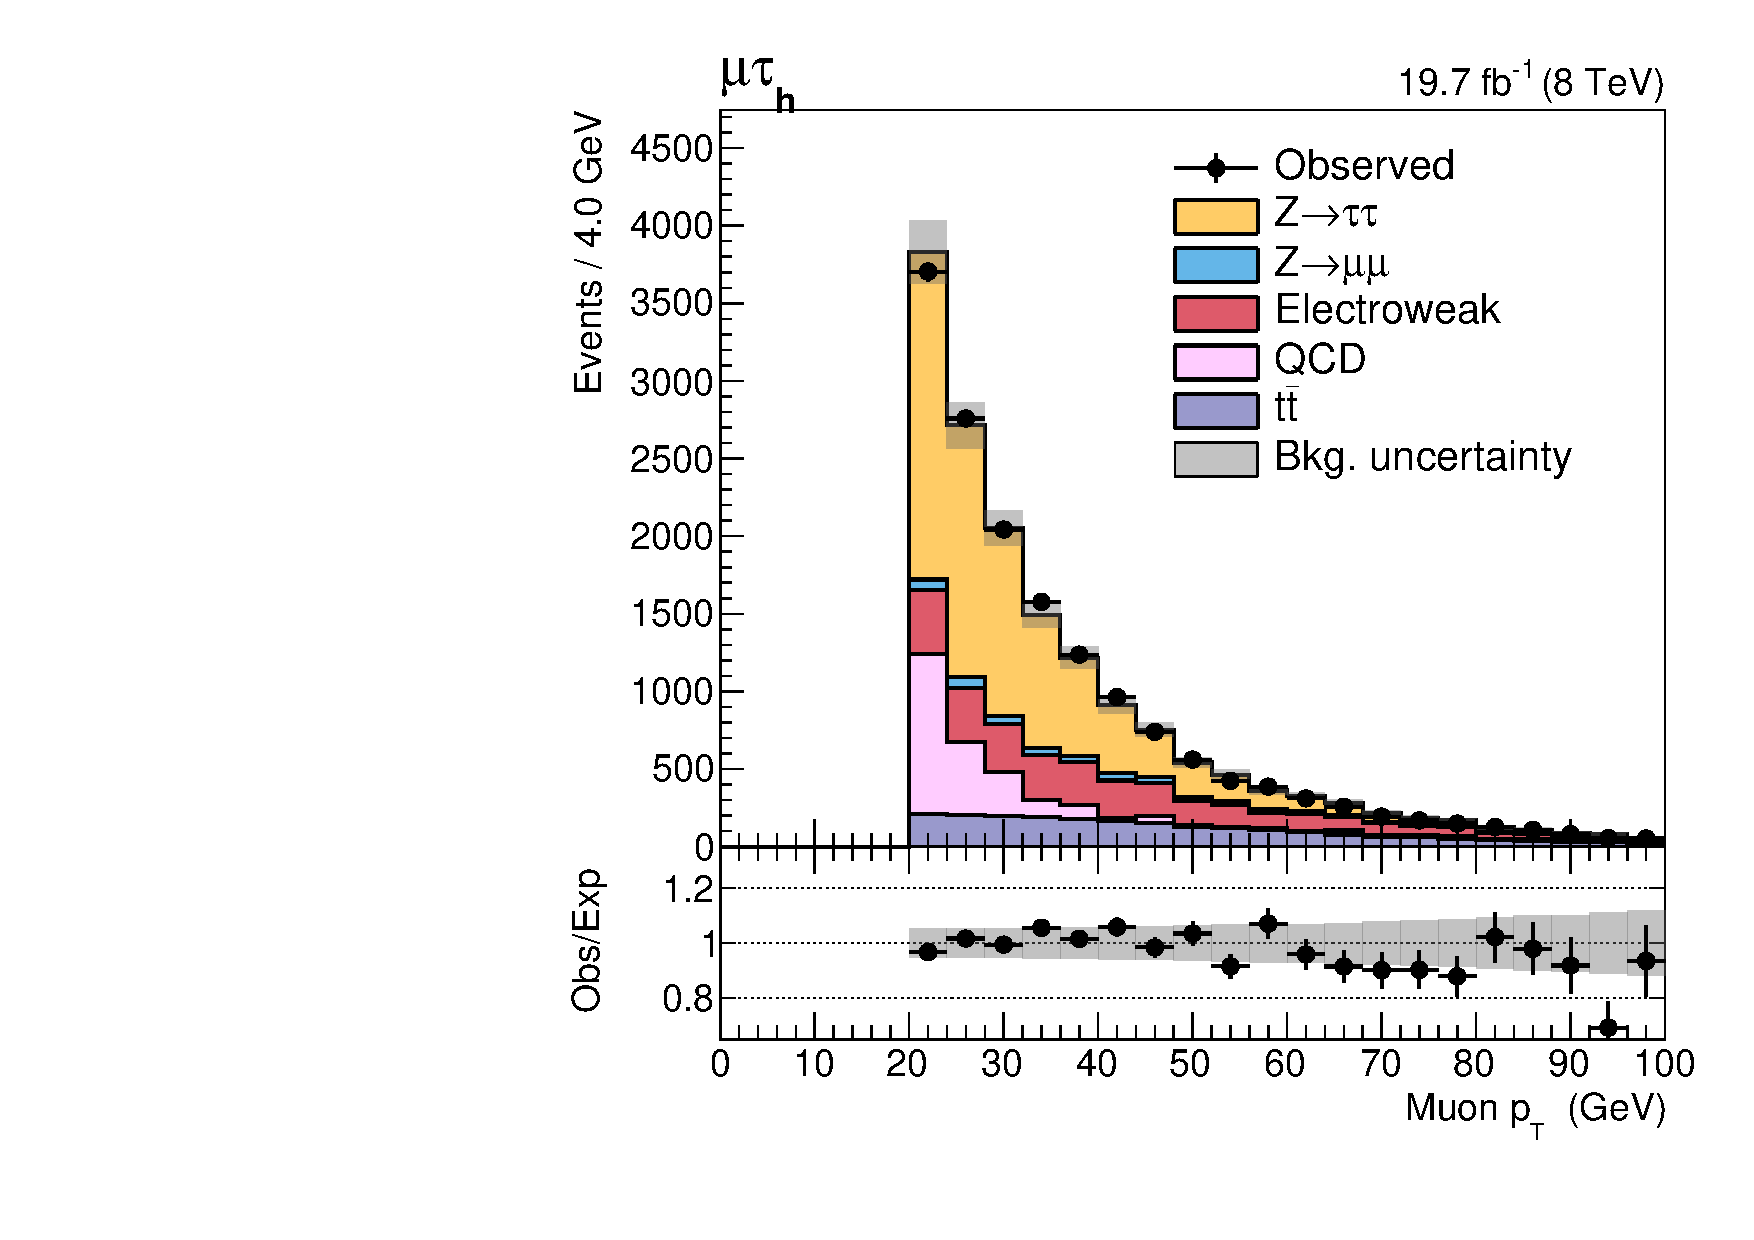
\includegraphics[width=0.5\textwidth]{Hhh/Plots/pt_1_2jetinclusive_mt_2012.pdf}}
%  \subfloat[Hadronic \Pgt \pT ]{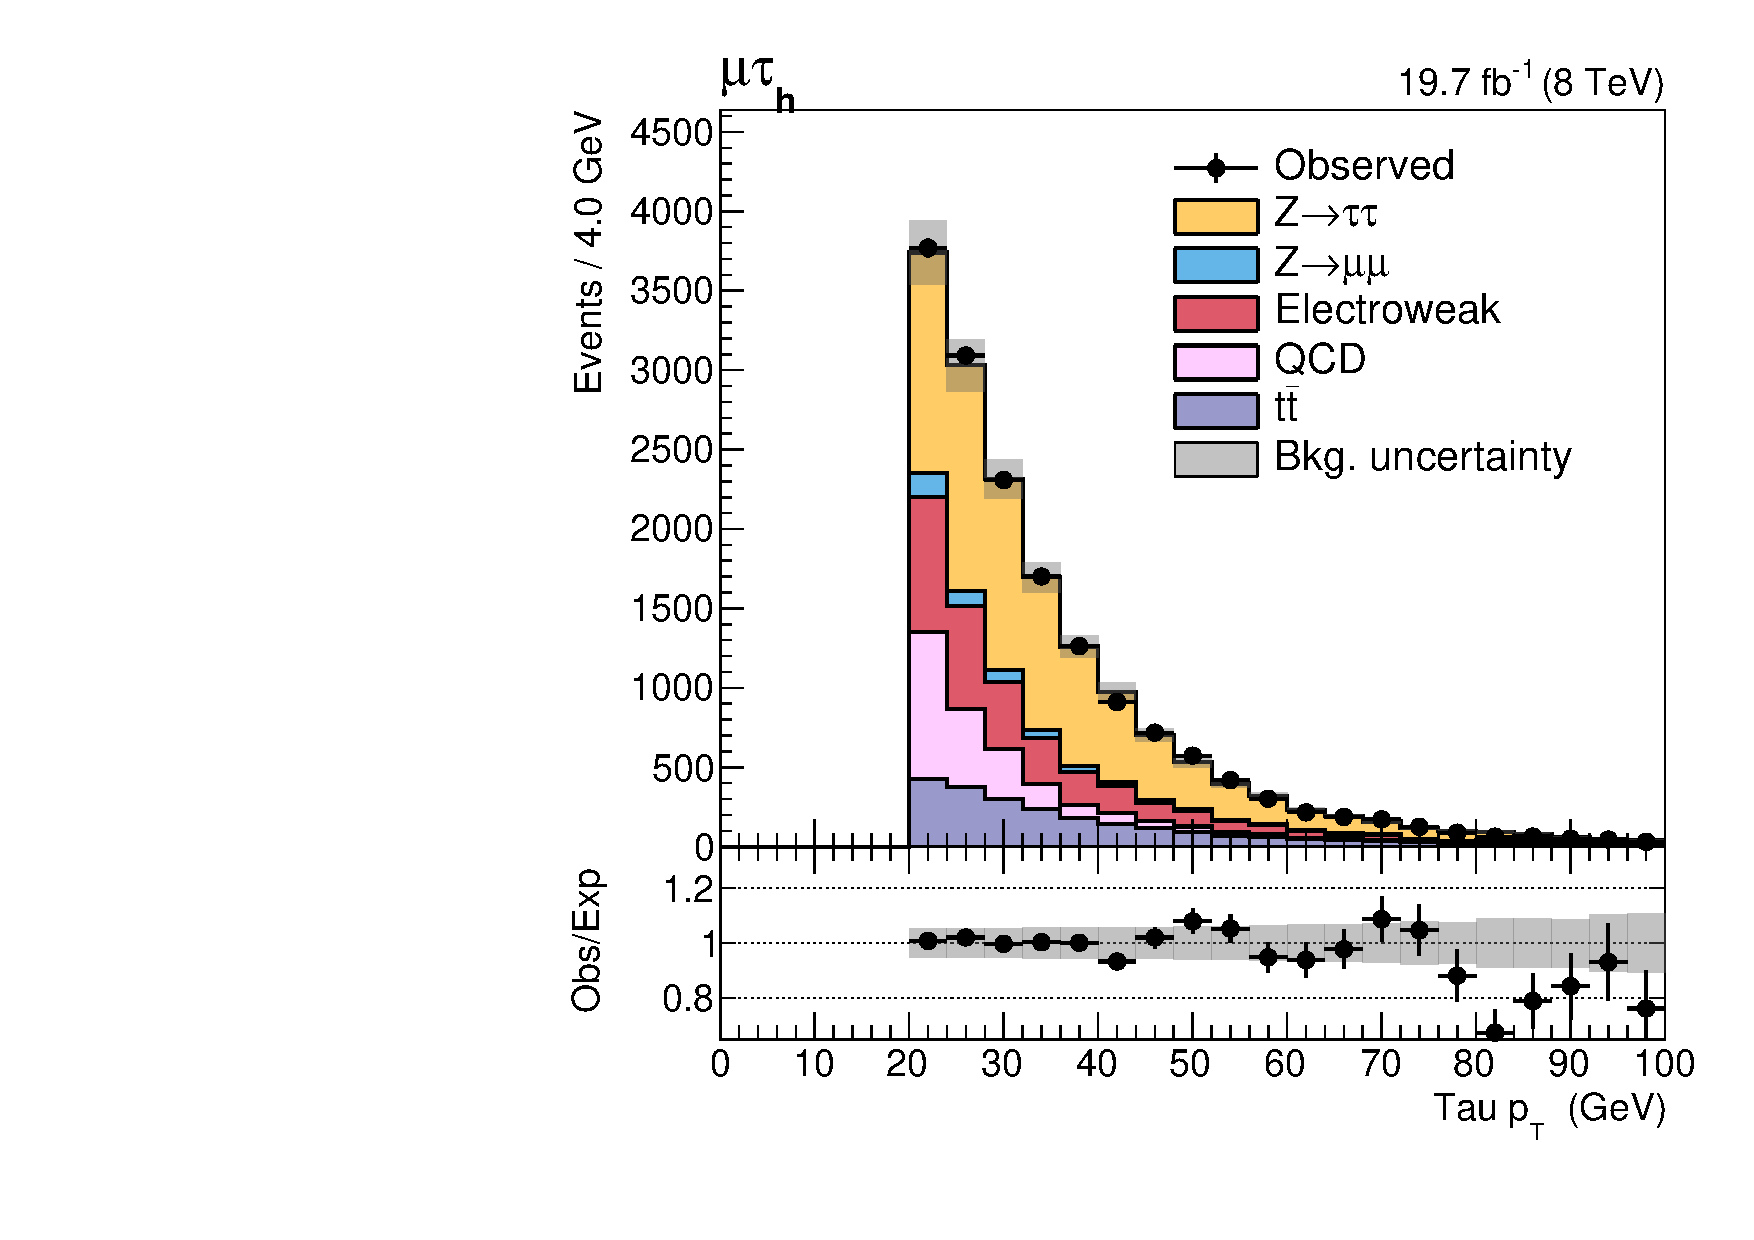
\includegraphics[width=0.5\textwidth]{Hhh/Plots/pt_2_2jetinclusive_mt_2012.pdf}}~\\
%  \subfloat[Muon $\eta$]{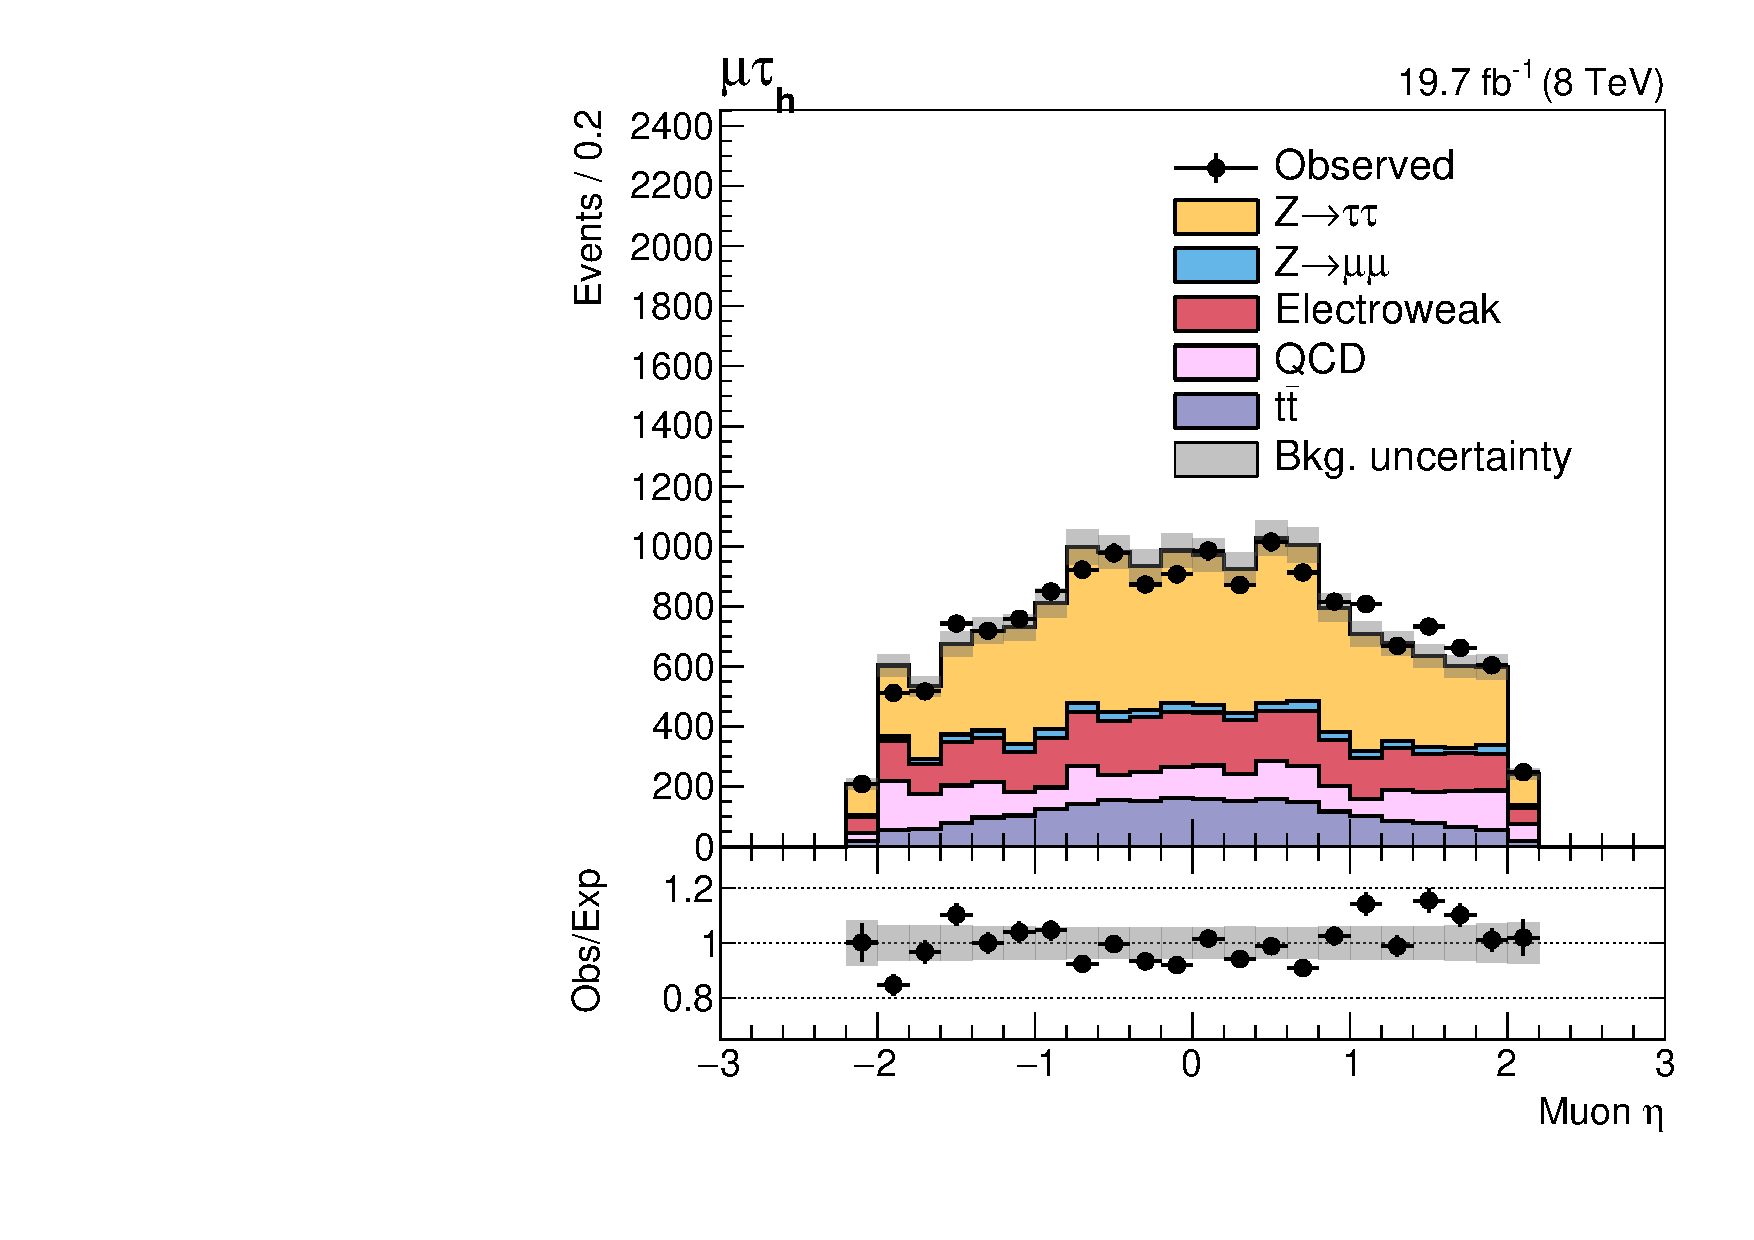
\includegraphics[width=0.5\textwidth]{Hhh/Plots/eta_1_2jetinclusive_mt_2012.pdf}}
%  \subfloat[Hadronic \Pgt $\eta$ ]{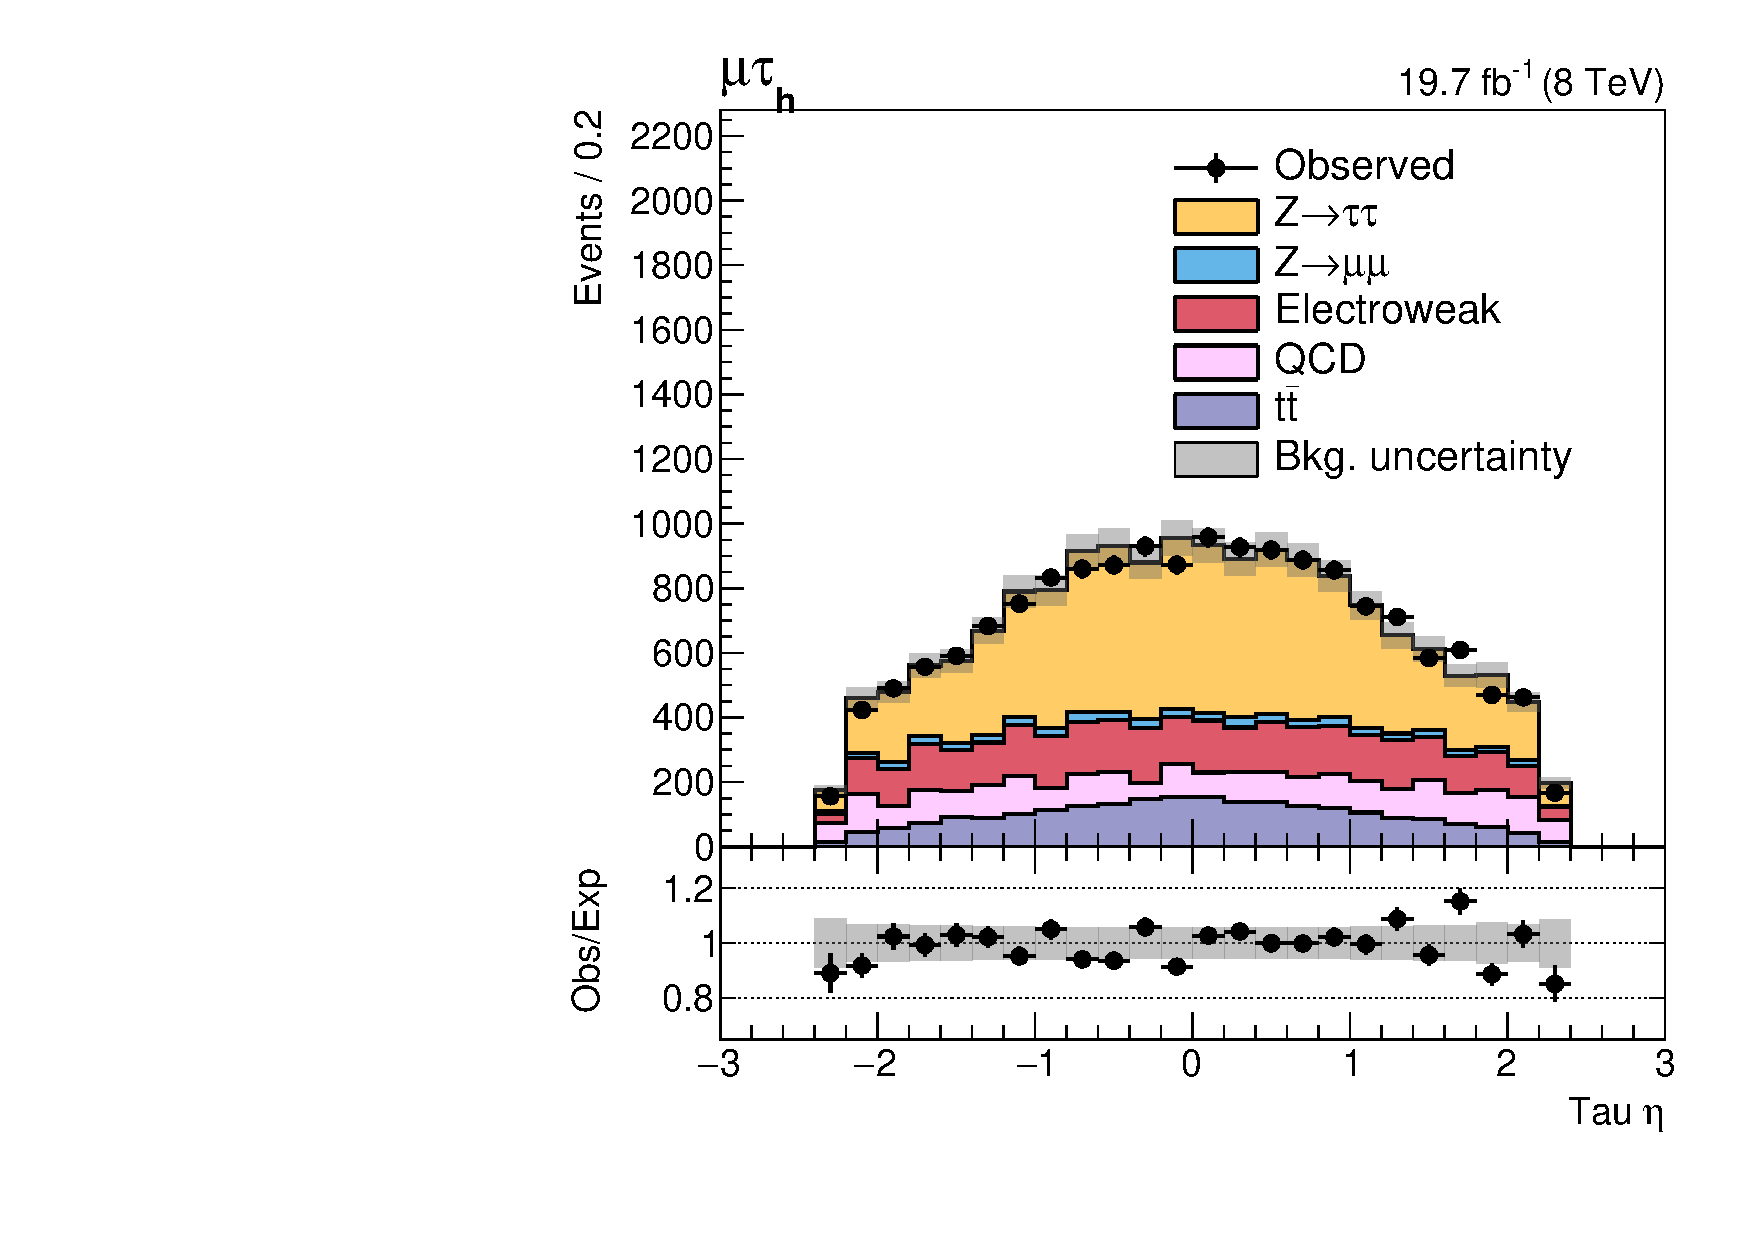
\includegraphics[width=0.5\textwidth]{Hhh/Plots/eta_2_2jetinclusive_mt_2012.pdf}}~\\
%
%\end{center}
%\caption{Plots of muon and hadronic \Pgt \pT and $\eta$ in the \mutau channel.}
%\label{fig:Hhh_selection_kinematics_mt}
%\end{figure}


\subsection{\texorpdfstring{Event selection in the \etau channel}{Event selection in the e-tau channel}}
\label{sec:hhh_selection_etau}
Events in the \etau channel are selected using a trigger which requires an electron at \ac{L1}, and both an electron
and a hadronic tau in the \ac{HLT}.
The hadronic
tau is reconstructed in a similar way as for the trigger in the \mutau channel, and loose ID and isolation requirements
are also applied to the electron at this stage.

After the trigger selection, an oppositely charged \etau pair is required, again separated by $\Delta R >0.5$. 
The electron should have a \pT~of at least $24\,\GeV$, $|\eta| < 2.1$, and should
satisfy $d_{xy} < 0.045\,\cm$ and $d_{z} < 0.2\,\cm$. The electron must pass the tight
working point of the electron MVA ID discriminator, and the
relative isolation is required to be $I_{\text{rel}}^{\Pe} < 0.1$. The requirements placed on the
hadronic tau are similar to those required in the \mutau channel, apart from the anti-muon discriminator,
where the loose working point is required, and the anti-electron discriminator, where the medium
working point of the MVA discriminator is required.

If there is more than one possible \etau pair, the pair with the largest \pT$^{\Pe}$+\pT$^{\Pgth}$
is taken. Similar additional vetoes as in the \mutau channel are applied.
The event is rejected if an opposite-charge pair of electrons with \pT~ $> 15\,\GeV$, passing looser ID and
isolation requirements than the signal electron requirements, can be formed. To prevent overlap with other channels and to reduce the di-boson
background, events that have more than one electron or at least one muon passing \pT~$>10\,\GeV$ and loose ID and isolation
requirements are rejected.

In addition to the requirements on the di-tau pair, at least two jets with \pT~$>20\,\GeV$ are 
required. 

%Figure \ref{fig:Hhh_selection_kinematics_etmt} shows some of the kinematic variables 
%of di-\Pgt candidates in the \etau and \mutau channels
%\begin{figure}[h!]
%\begin{center}
% \subfloat[Electron \pT (\etau)]{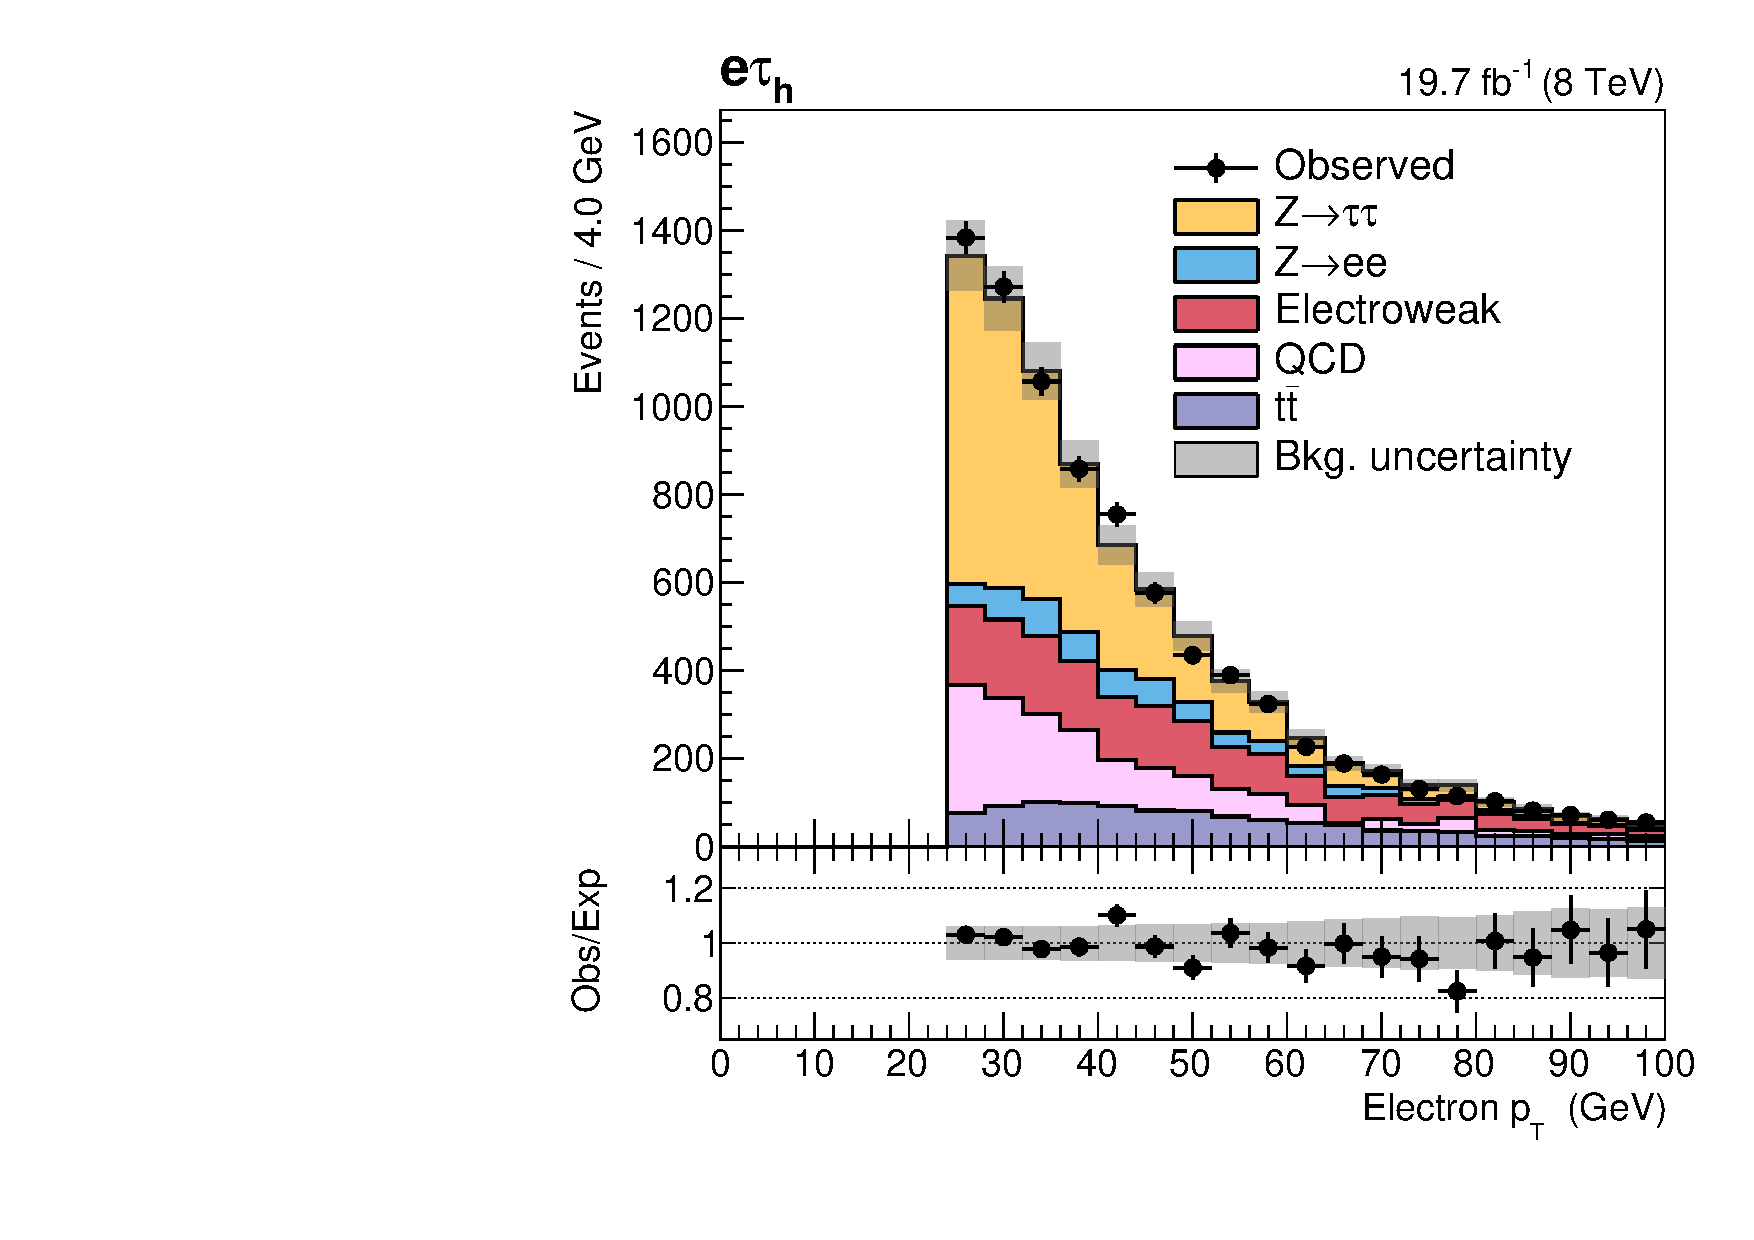
\includegraphics[width=0.5\textwidth]{Hhh/Plots/pt_1_2jetinclusive_et_2012.pdf}}
%  \subfloat[Hadronic \Pgt \pT (\mutau)]{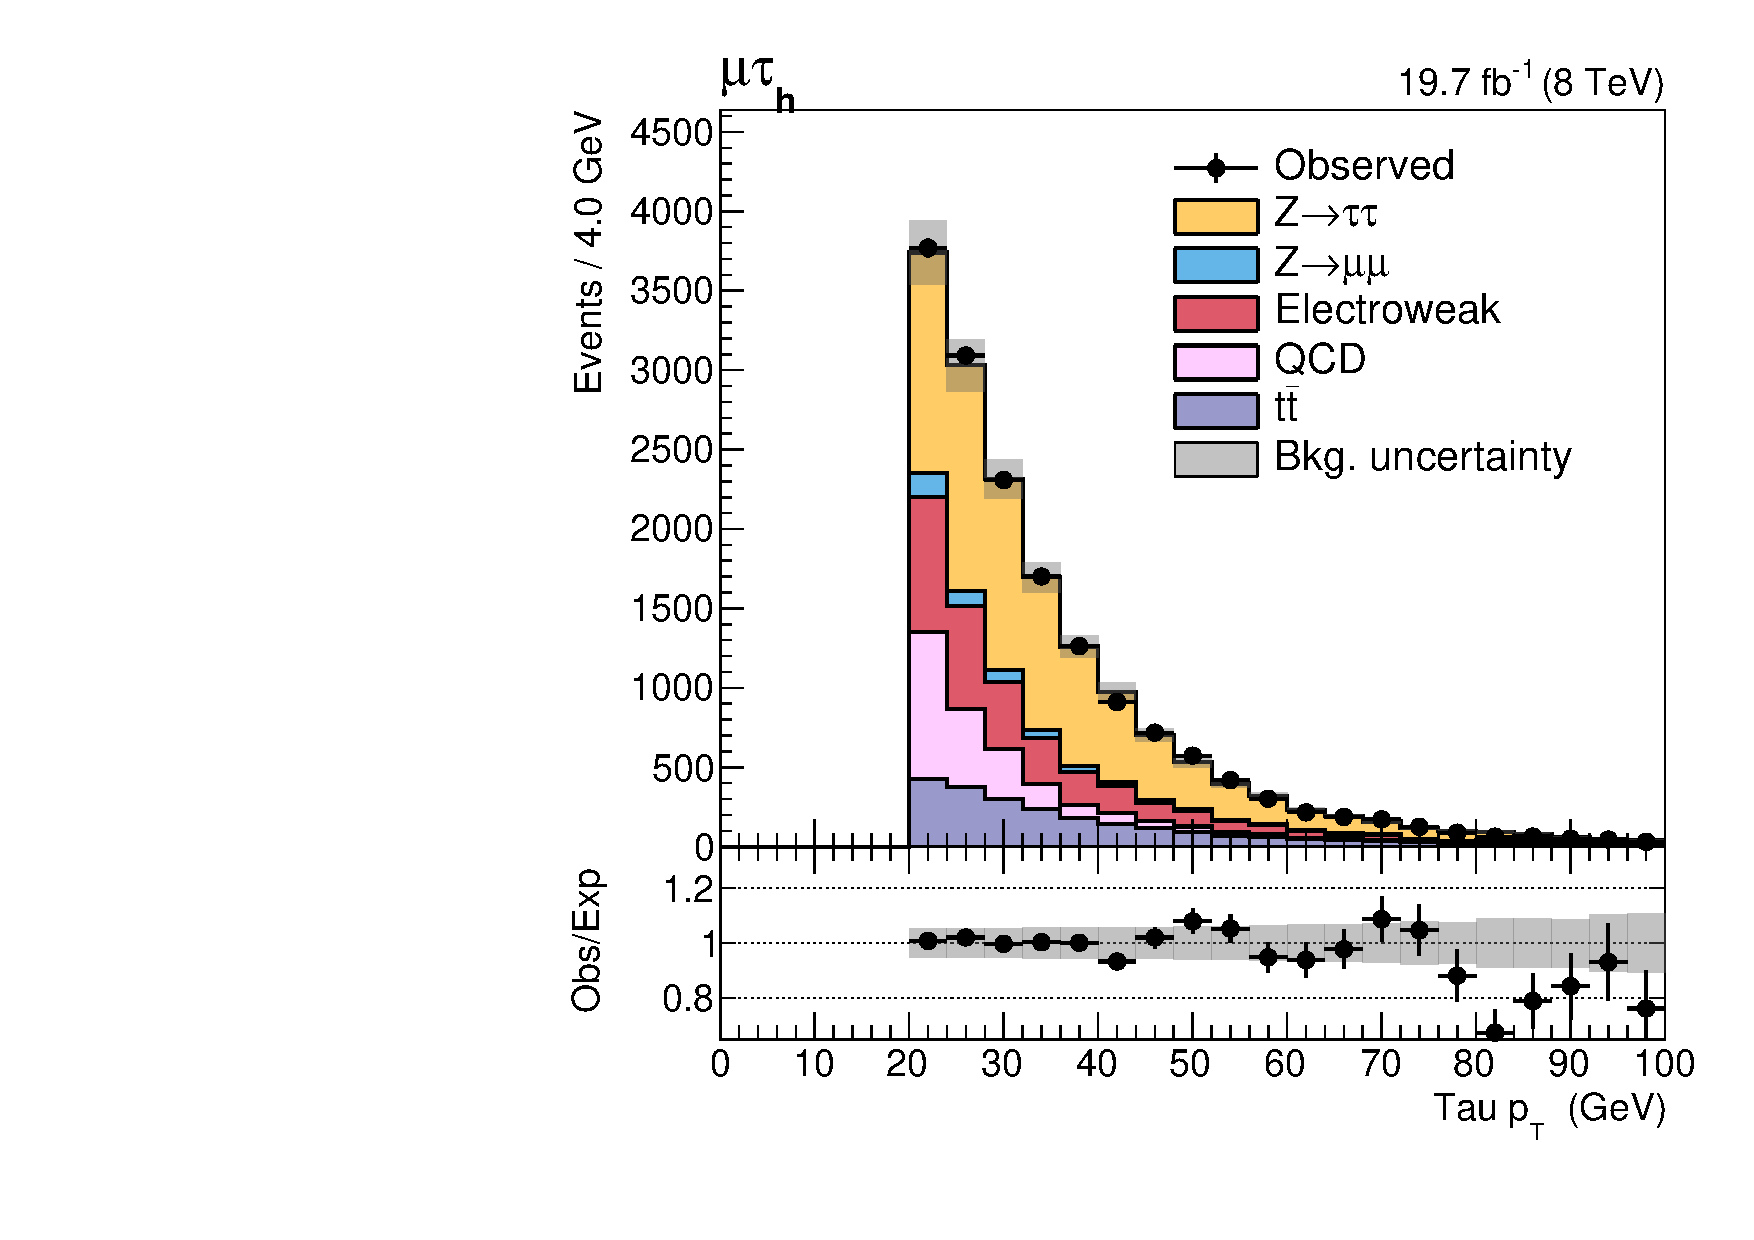
\includegraphics[width=0.5\textwidth]{Hhh/Plots/pt_2_2jetinclusive_mt_2012.pdf}}
%  \subfloat[Electron $\eta$]{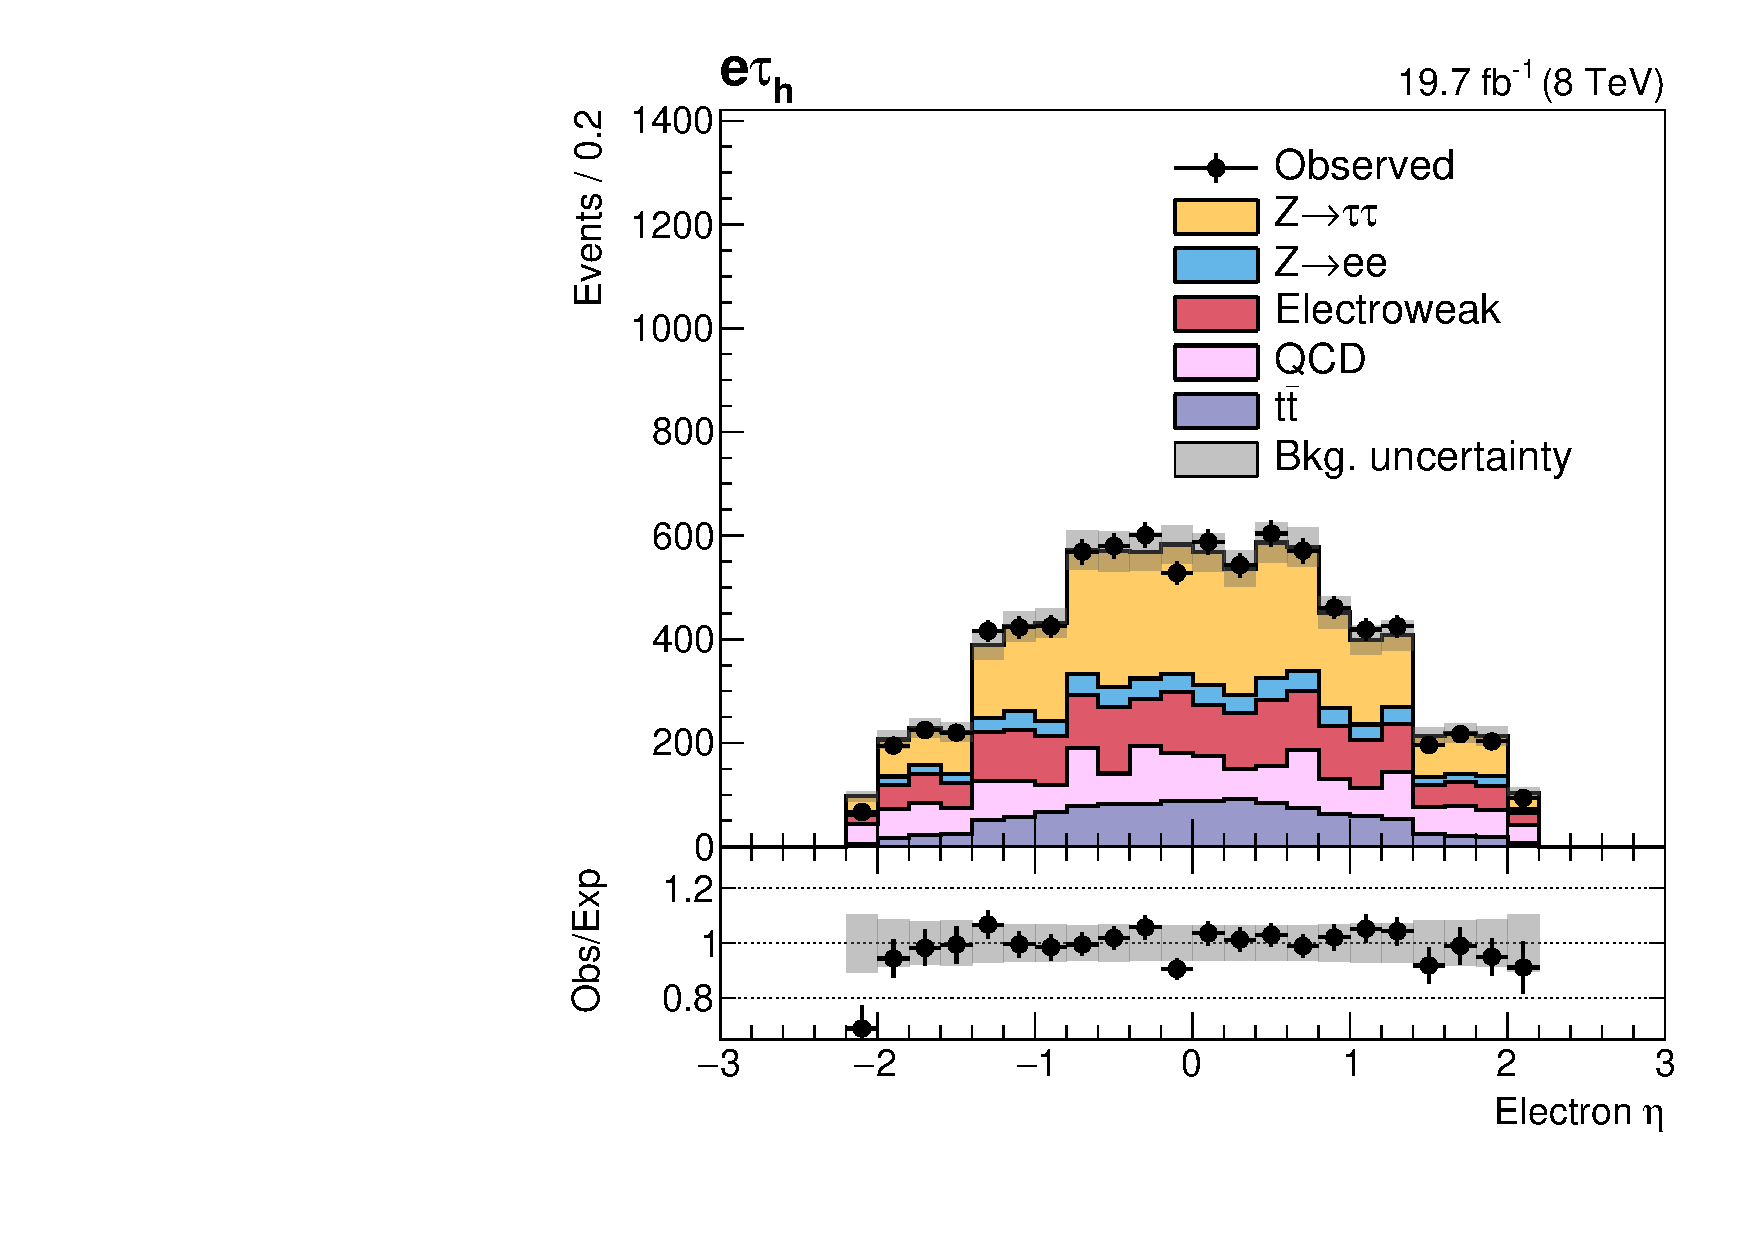
\includegraphics[width=0.5\textwidth]{Hhh/Plots/eta_1_2jetinclusive_et_2012.pdf}}
%  \subfloat[Hadronic \Pgt $\eta$ ]{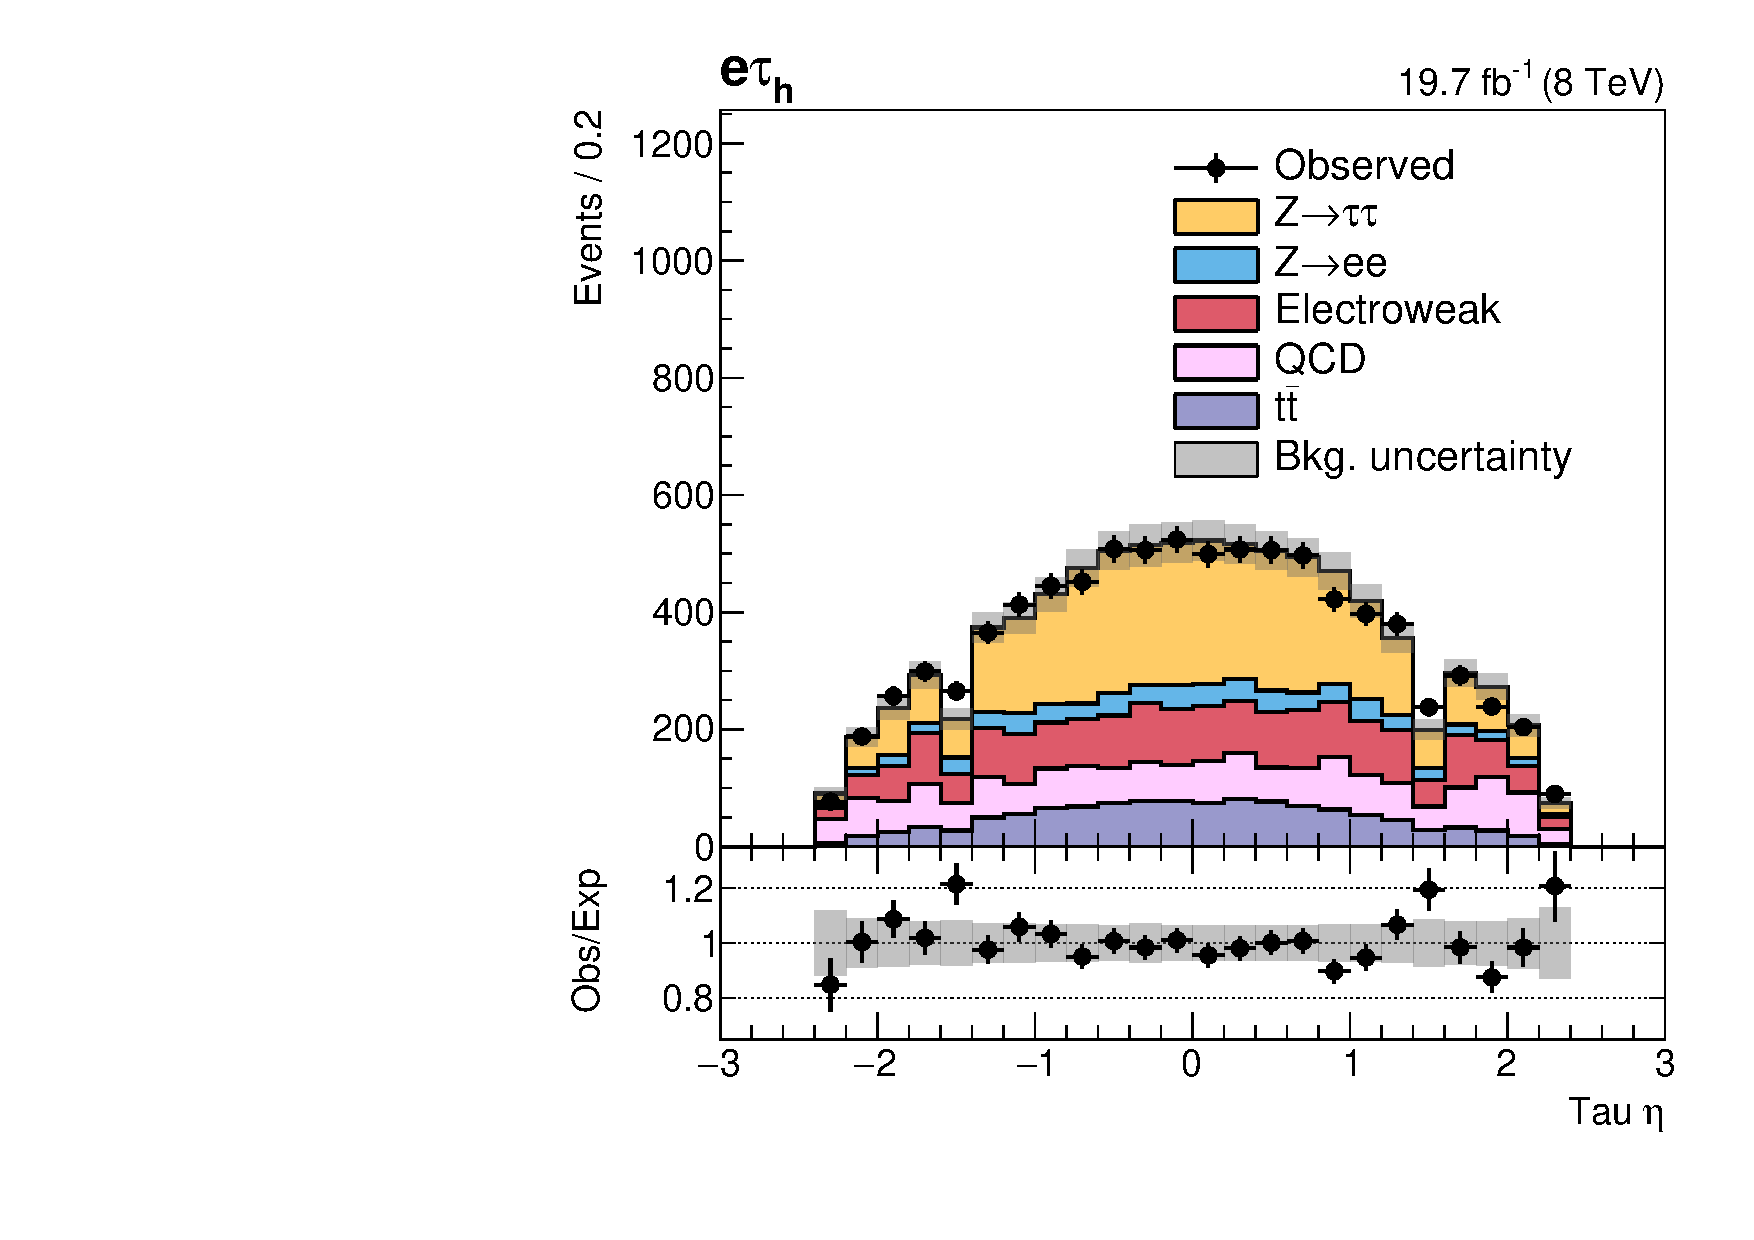
\includegraphics[width=0.5\textwidth]{Hhh/Plots/eta_2_2jetinclusive_et_2012.pdf}}~\\

%\end{center}
%\caption{Plots of electron \pT in the \etau channel and hadronic \Pgt \pT in the \mutau channel.}
%\label{fig:Hhh_selection_kinematics_etmt}
%\end{figure}

\subsection{Categorisation}
\label{sec:hhh_selection_categories}
In both channels a selection on the transverse mass, \mT, between the electron or muon
and missing transverse energy, defined as,
\begin{equation}\label{eqn:hhh_selection_mt}
m_{\text{T}} = \sqrt{2p_{\text{T}}E_{\text{T}}^{\text{miss}}(1-\cos{\Delta\phi})}\,,
\end{equation}
is applied.
In this eqation \pT~is the transverse momentum of the electron or muon, and $\Delta\phi$ the azimuthal
angle between this light lepton and the missing transverse energy. The \mT~distributions for the \etau
and \mutau channels, using the selections as
described in sections \ref{sec:hhh_selection_mutau} and \ref{sec:hhh_selection_etau},
are shown in figure \ref{fig:Hhh_selection_mt}.

\begin{figure}[h!]
\begin{center}
\subfloat[\mutau channel]{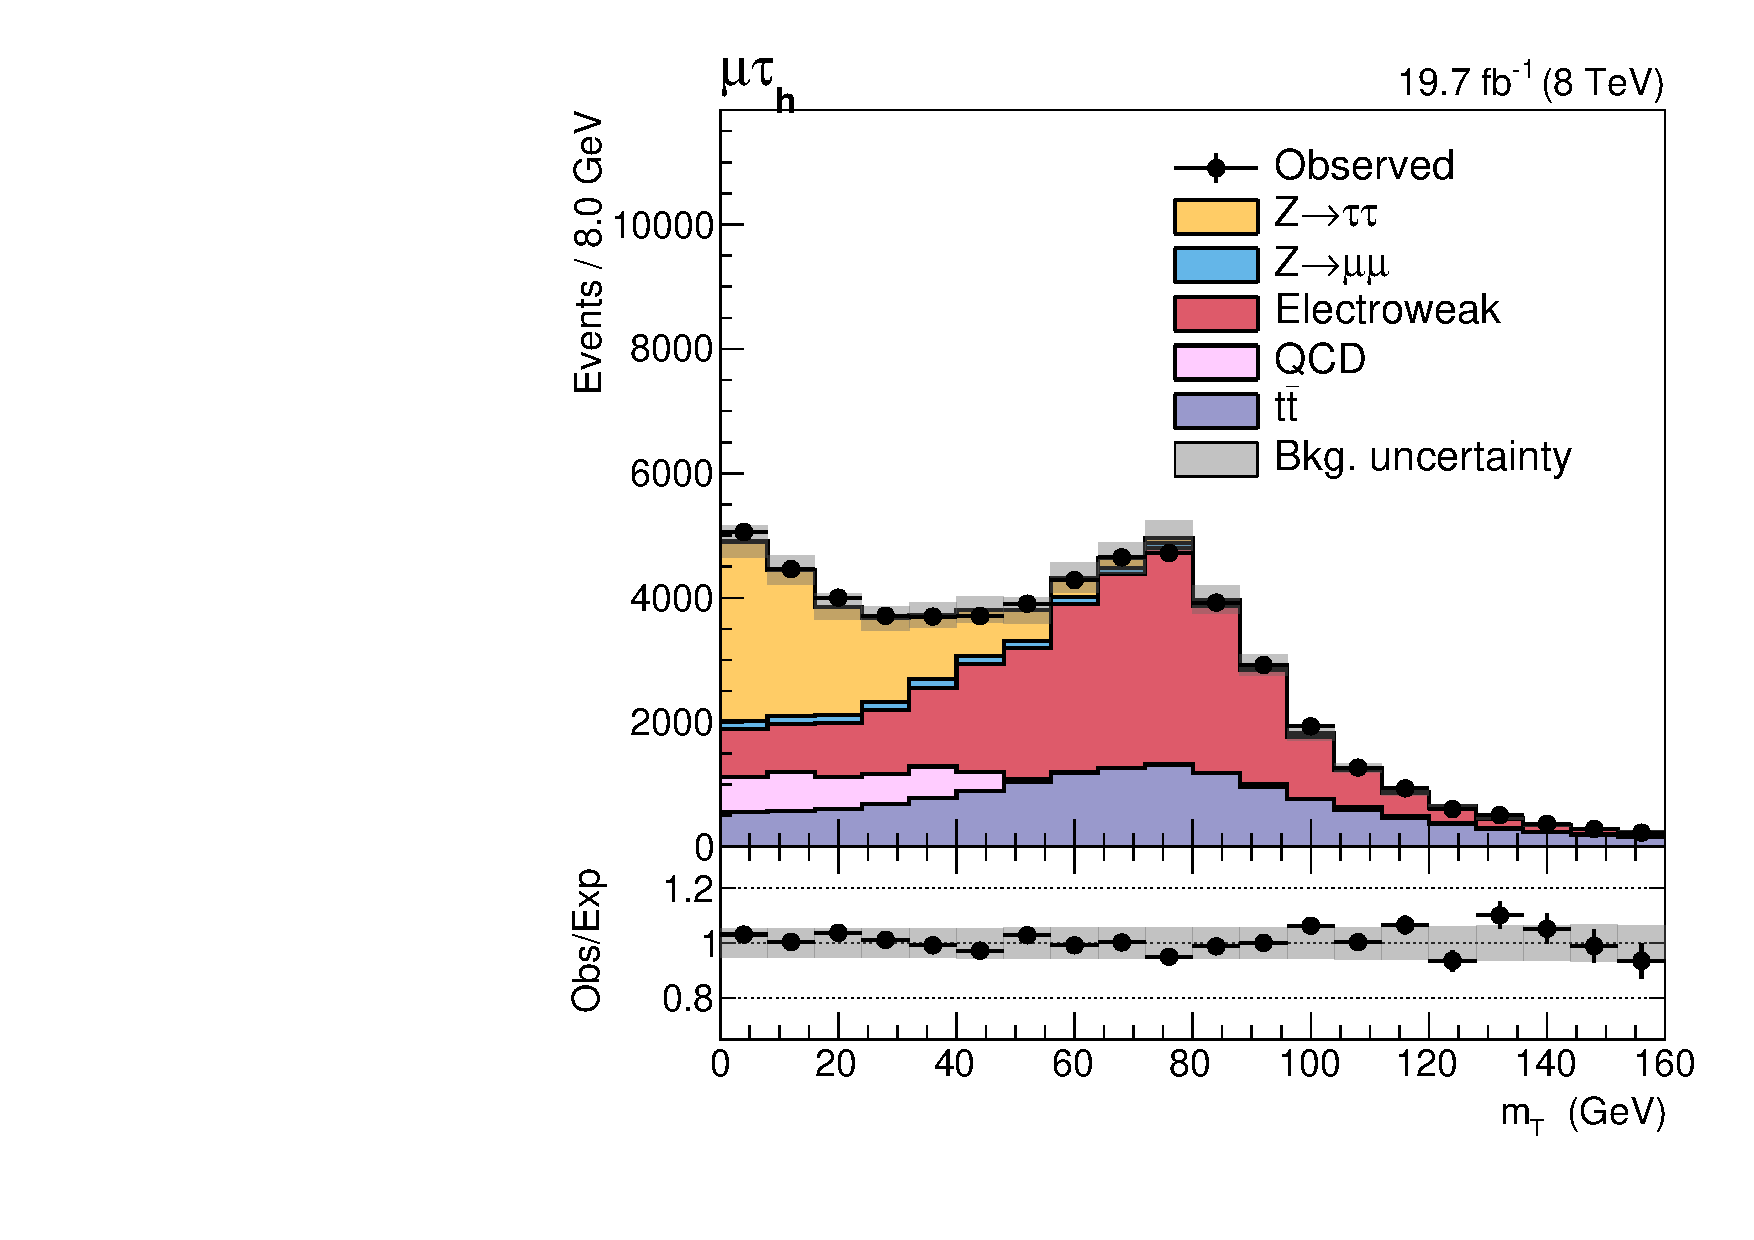
\includegraphics[width=0.5\textwidth]{Hhh/Plots/mt_1_2jetinclusive_mt_2012.pdf}}
\subfloat[\etau channel]{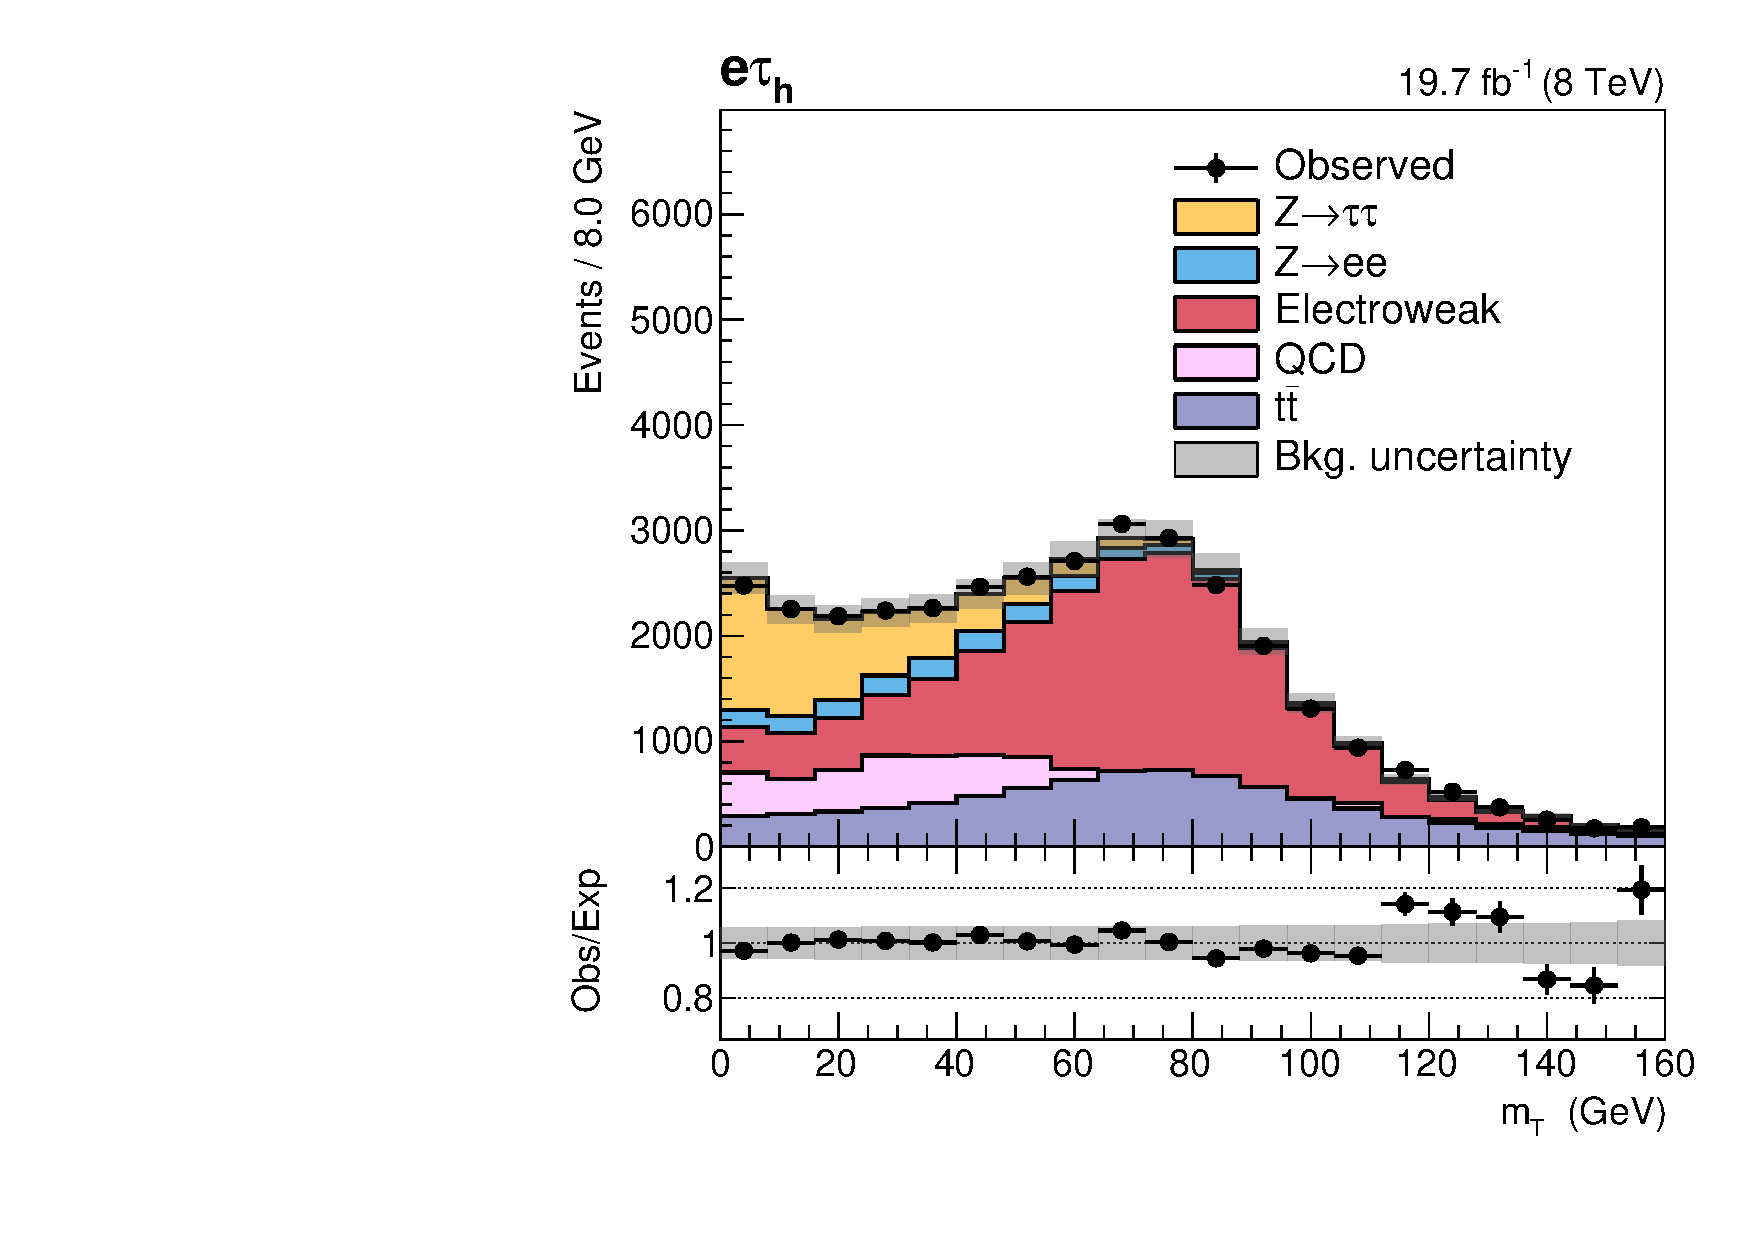
\includegraphics[width=0.5\textwidth]{Hhh/Plots/mt_1_2jetinclusive_et_2012.pdf}}
\end{center}
\caption[\mT~distributions in the \mutau and \etau channels.]{\mT~distributions in the (a) \mutau and (b) \etau channels.}
\label{fig:Hhh_selection_mt}
\end{figure}

This quantity is required to be smaller than $30\,\GeV$ in both channels. In events
where the missing energy and the light lepton are oriented back-to-back, \mT~is
large, whereas it is closer to zero when the two are aligned. In $\PW\rightarrow\ell\nu$
events, as the \PW boson is very heavy, the lepton and neutrino are more likely to be emitted back-to-back,
therefore \mT~will be large. For \Ztautau and \htotautau events, the neutrinos in the $\tau\rightarrow\ell\nu\nu$ decay 
 are more likely to travel in the same direction as the visible decay products of 
the tau, due to the smaller mass of the \Pgt compared with the \PW boson. Therefore requiring the
transverse mass to be less than $30\,\GeV$ reduces the \Wjets background. This effect
is also visible in figure \ref{fig:Hhh_selection_mt}, where the \Wjets and the much
smaller di-boson and single-top backgrounds are combined into the ``electroweak'' background contribution, drawn in red.
%In this analysis the presence of at least 2 jets increases the relative fraction of \ttbar 
%background events. Because the missing energy can now originate from multiple
%heavy objects (two tops) the missing transverse energy alignment is randomised. In some
%cases the lepton and missing transverse energy can be very much like the W decay
%topology, whereas in other cases \mT will be lower

After applying the \mT~selection, events are divided into three categories to maximise
sensitivity to the signal: 2jet-0tag (at least two jets, none of which are b-tagged), 2jet-1tag 
(at least two jets, exactly one of which is b-tagged), 2jet-2tag (at least two jets, at least two of which are b-tagged).
Jets are considered b-tagged if they pass the medium working point of the \ac{CSV} b-tagging discriminator.
The 2jet-0tag category does not collect much of the signal and is dominated by 
backgrounds, the 2jet-2tag category is the most sensitive to signal. 
Figure \ref{fig:Hhh_selection_bjets}, which shows the number of b-tagged jets in the two-jet selection of the \mutau and \etau
channels, illustrates this.

\begin{figure}[h!]
\begin{center}
\subfloat[\mutau channel]{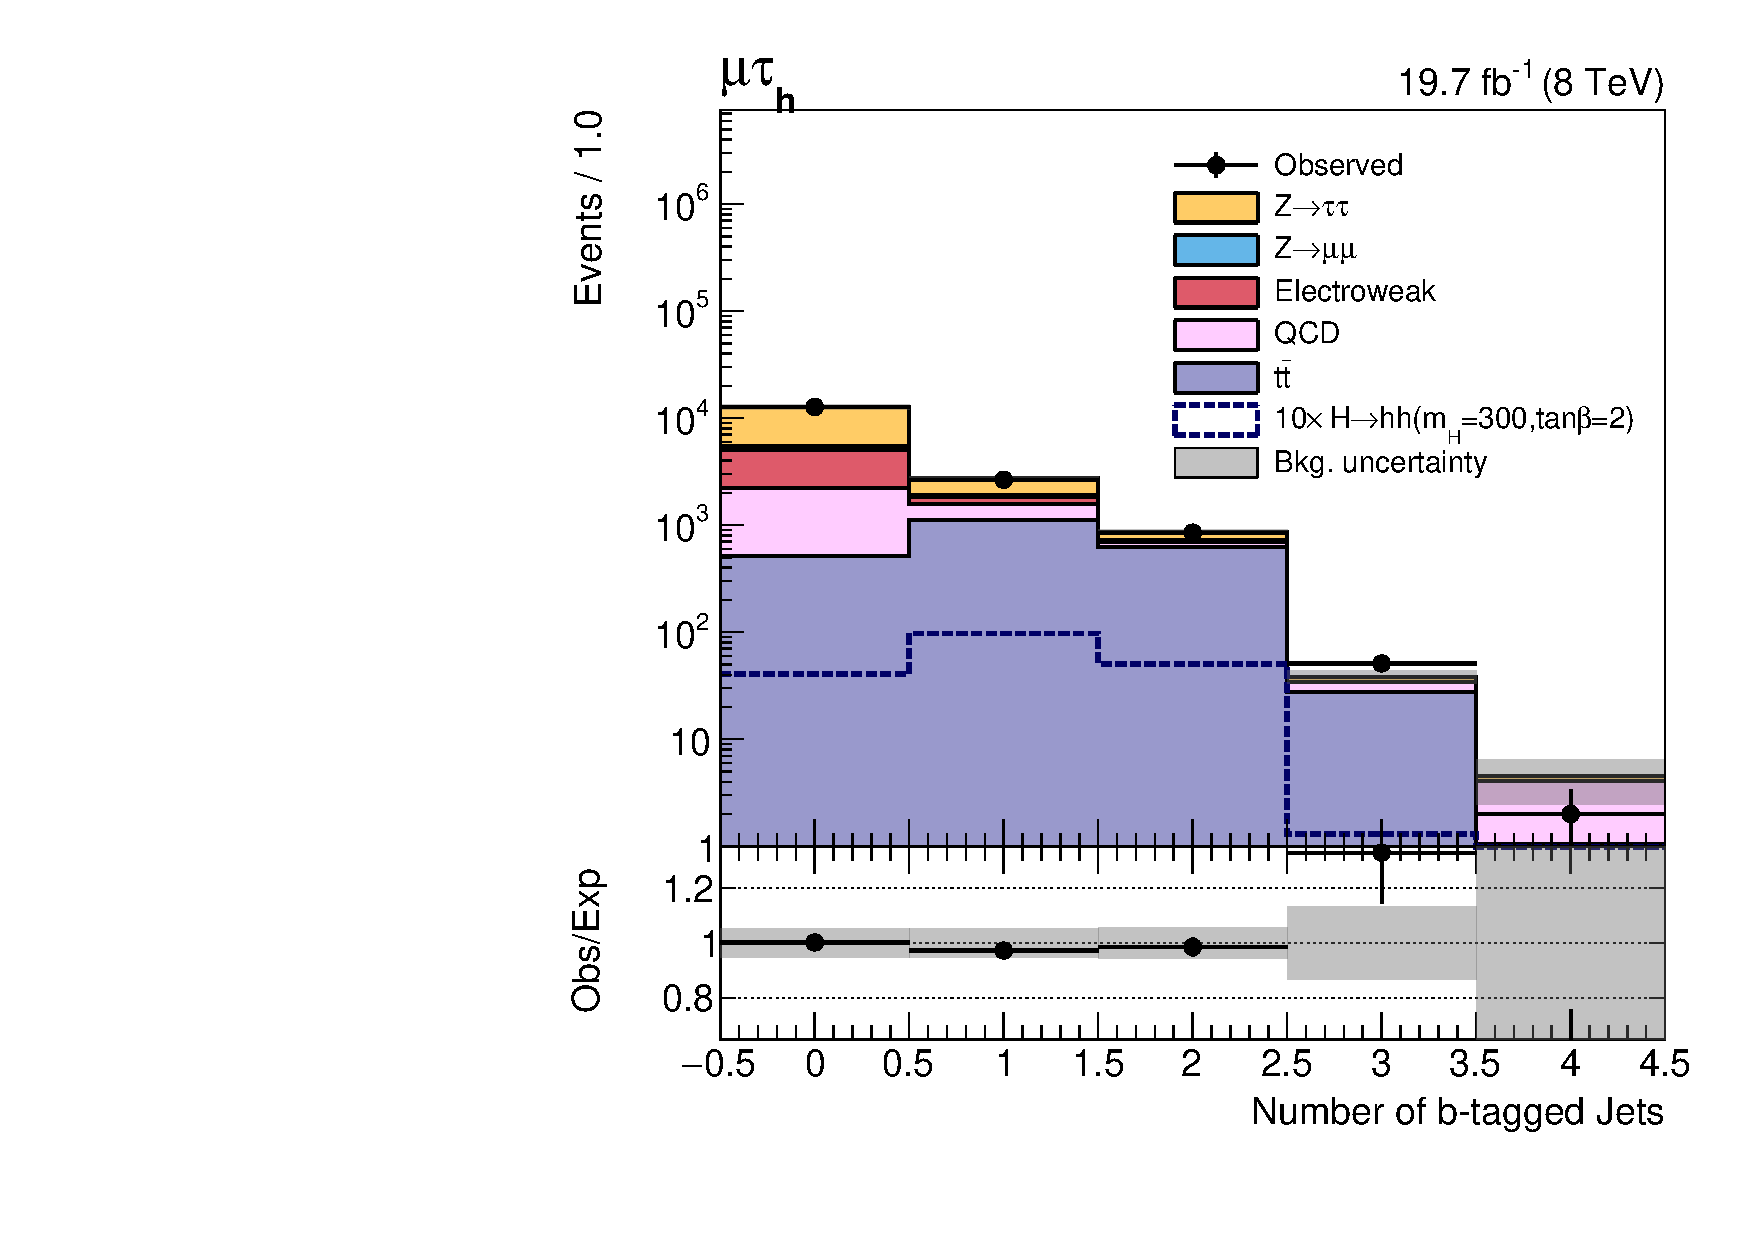
\includegraphics[width=0.5\textwidth]{Hhh/Plots/n_bjets_csv_2jetinclusive_mt_2012_log.pdf}}
\subfloat[\etau channel]{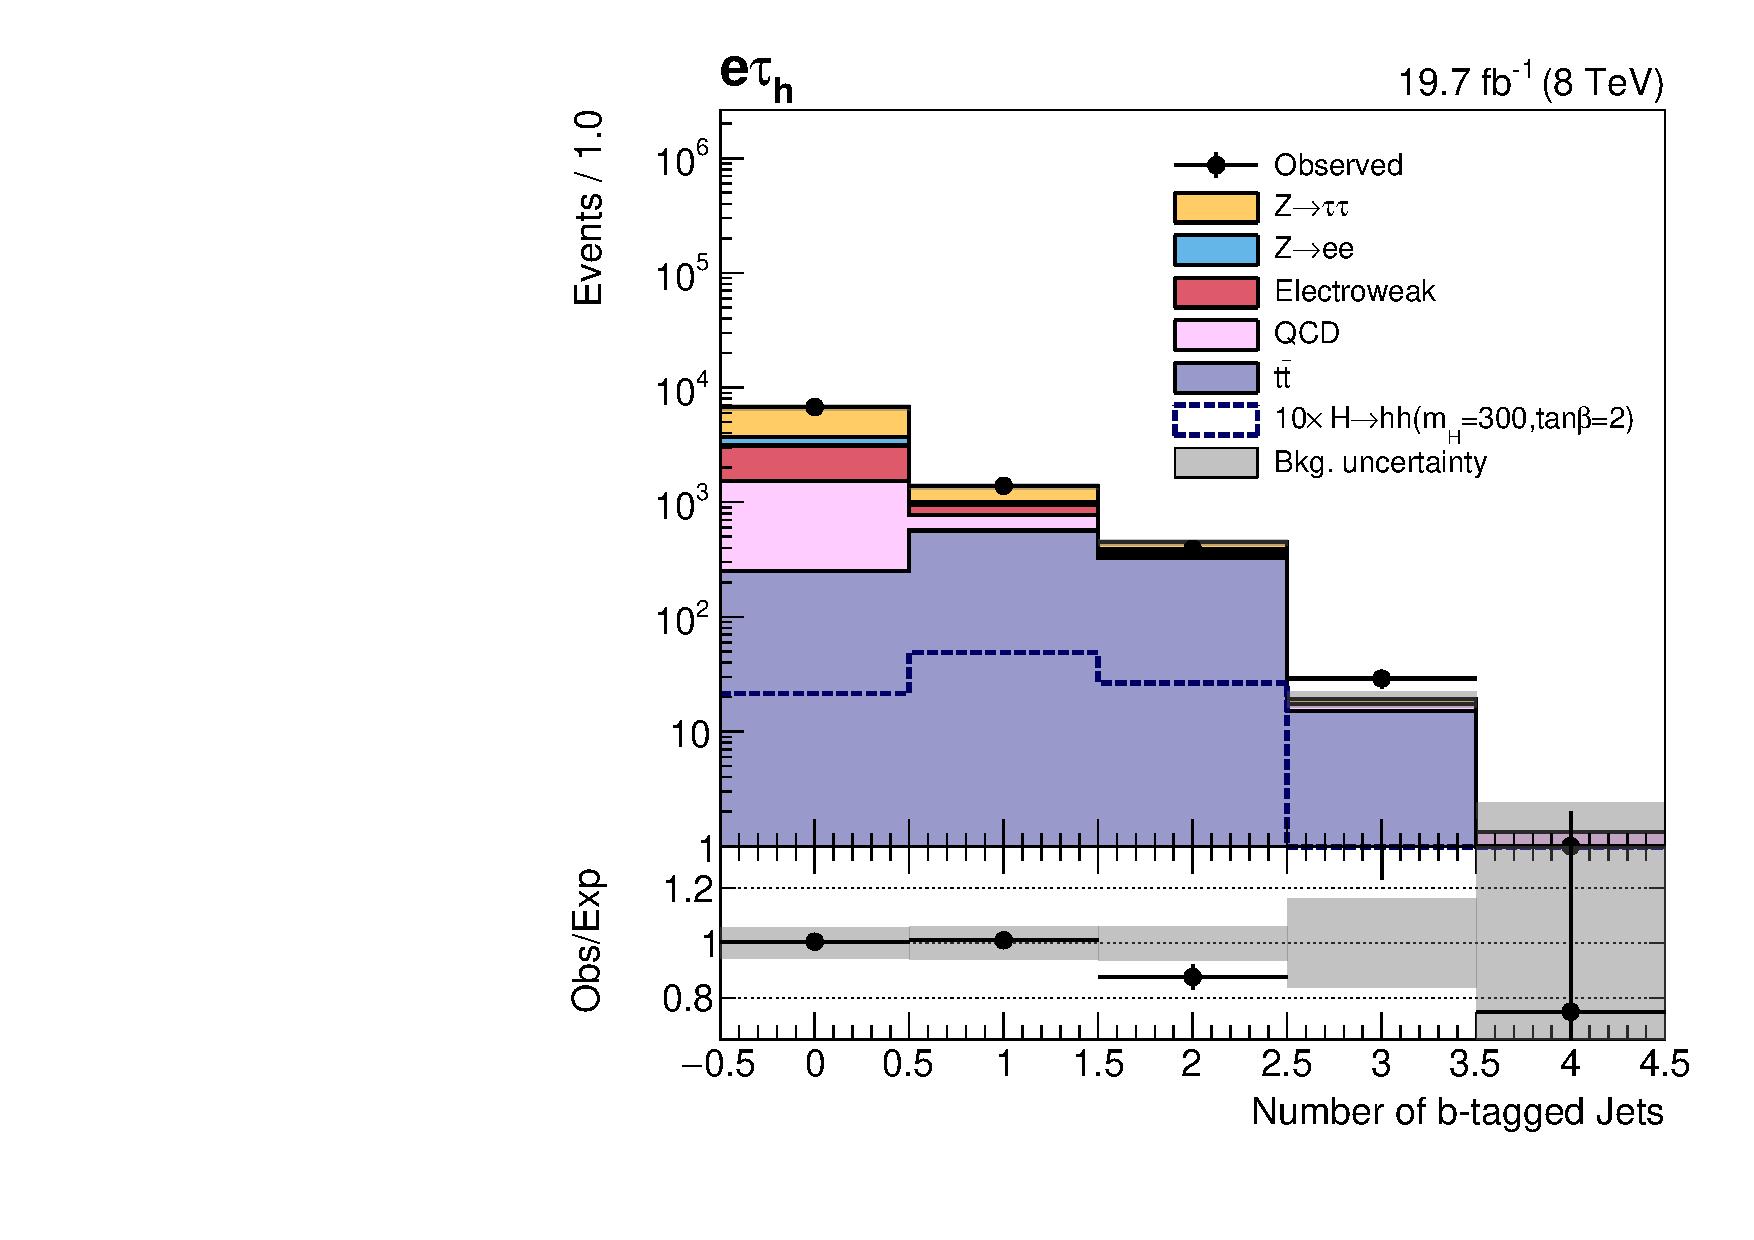
\includegraphics[width=0.5\textwidth]{Hhh/Plots/n_bjets_csv_2jetinclusive_et_2012_log.pdf}}
\end{center}
\caption[Number of b-tagged jets in the two-jet selection of the \mutau and \etau channels.]{Number of b-tagged jets in the two-jet selection of the (a) \mutau and (b) \etau channels. The signal
at \mH~$=300\,\GeV$ and \tanb~$=2$ in the \ac{MSSM} low-\tanb~scenario, multiplied by a factor of 10, is overlaid.}
\label{fig:Hhh_selection_bjets}
\end{figure} 

In signal events the di-tau pair and di-jet pair 
are the decay products of a $125\,\GeV$ Higgs boson, therefore their invariant
masses should be close to $125\,\GeV$. To reduce background contributions
from events where the di-tau or di-jet mass is not compatible with
$125\,\GeV$, requirements are made on the di-jet invariant mass, and the di-tau
invariant mass as reconstructed using the \texttt{SVFit} algorithm \cite{HDiscoveryCMS,SVFit}. This algorithm provides
a likelihood-based estimate of the di-tau mass using the visible decay products
of the taus and the reconstructed \MET. The use of this algorithm greatly
improves the separation between $\PZ\rightarrow\Pgt\Pgt$ and $\PHiggs\rightarrow\Pgt\Pgt$ events, 
which is of great importance for the \ac{SM} $\PHiggs\rightarrow\Pgt\Pgt$ analysis \cite{HDiscoveryCMS}.
By requiring $70 < m_{jj} < 150\,\GeV$ and $90 < m_{\Pgt\Pgt} < 150\,\GeV$ a 
large number of background events can be rejected, while retaining
most of the signal. This is illustrated in figure \ref{fig:Hhh_selection_masscuts} for 
the 2jet-2tag category.

\begin{figure}[h!]
\begin{center}
\subfloat[$m_{\Pgt\Pgt}$]{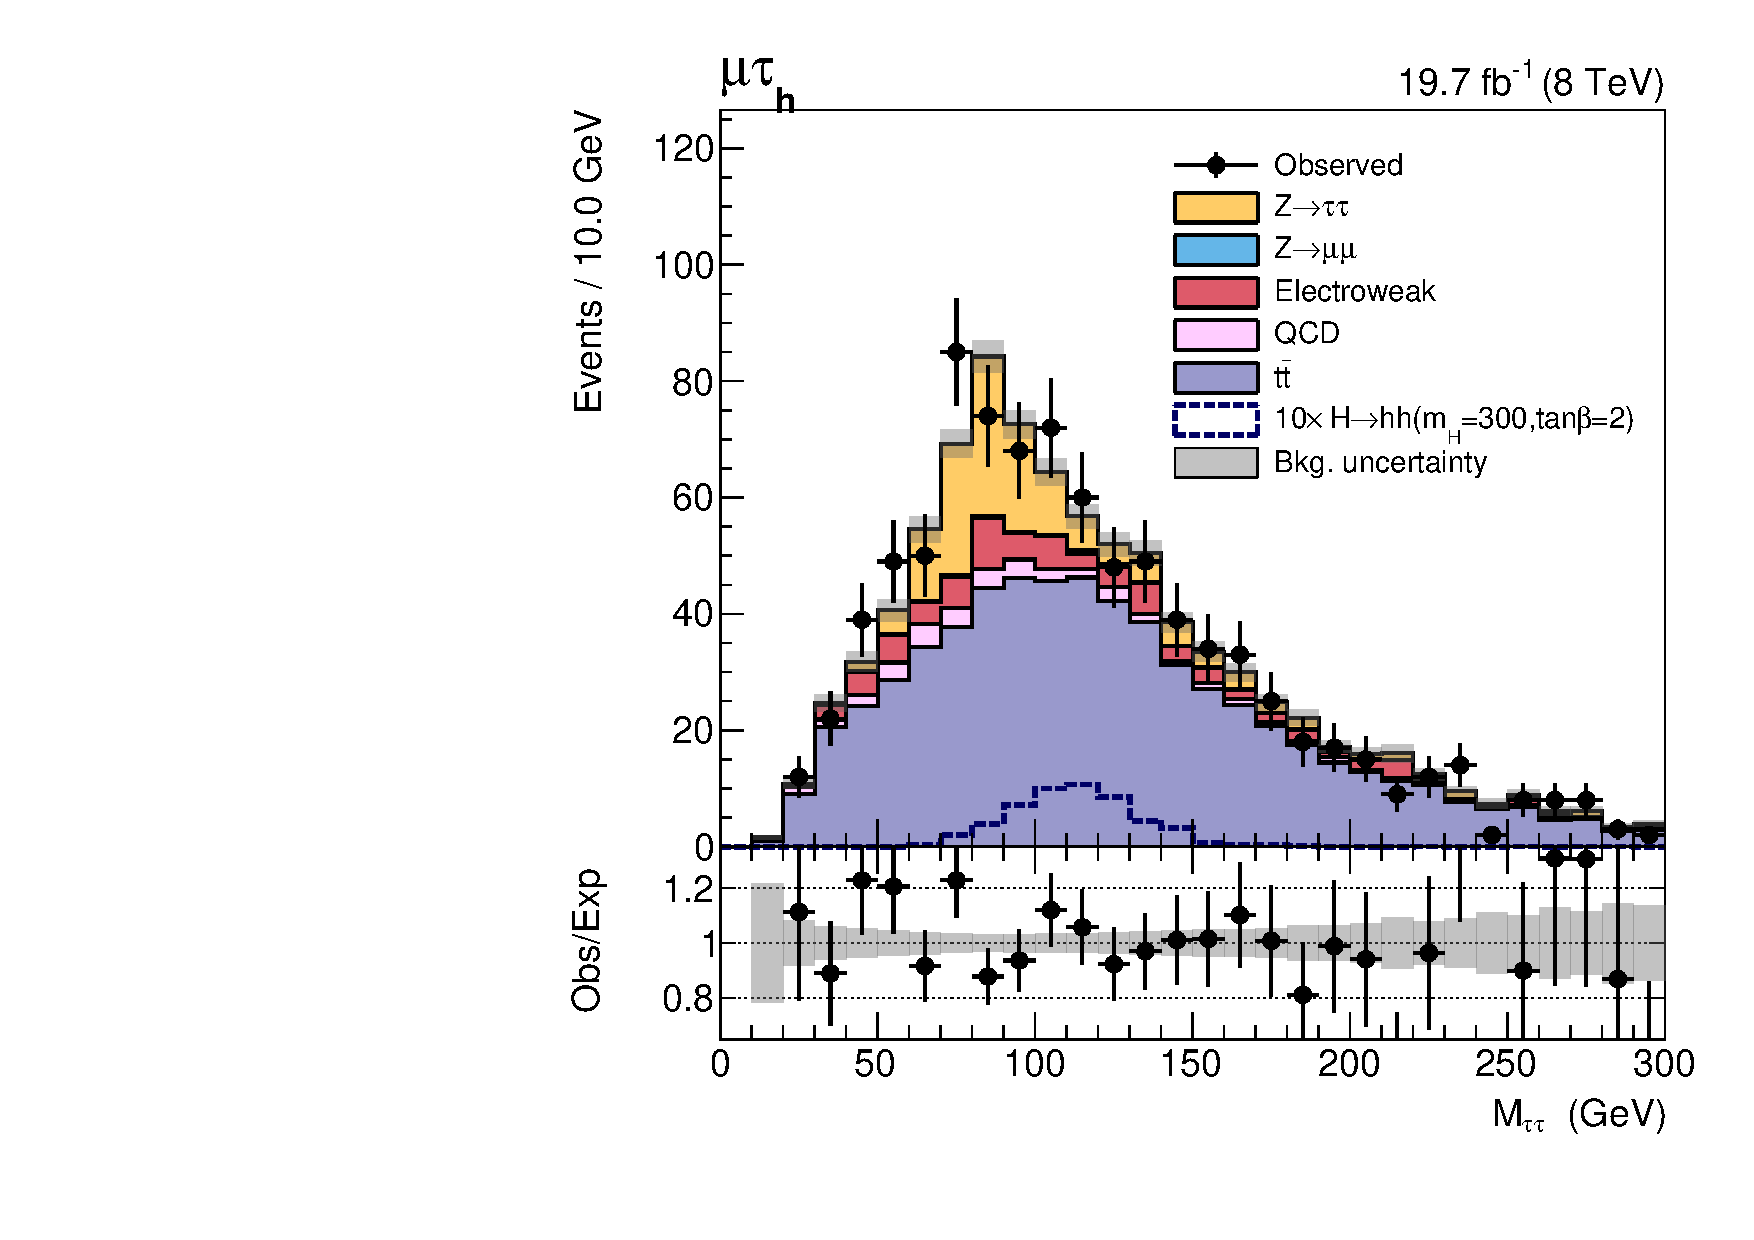
\includegraphics[width=0.5\textwidth]{Hhh/Plots/m_sv_2jet2tag_mt_2012.pdf}}
\subfloat[$m_{jj}$ ]{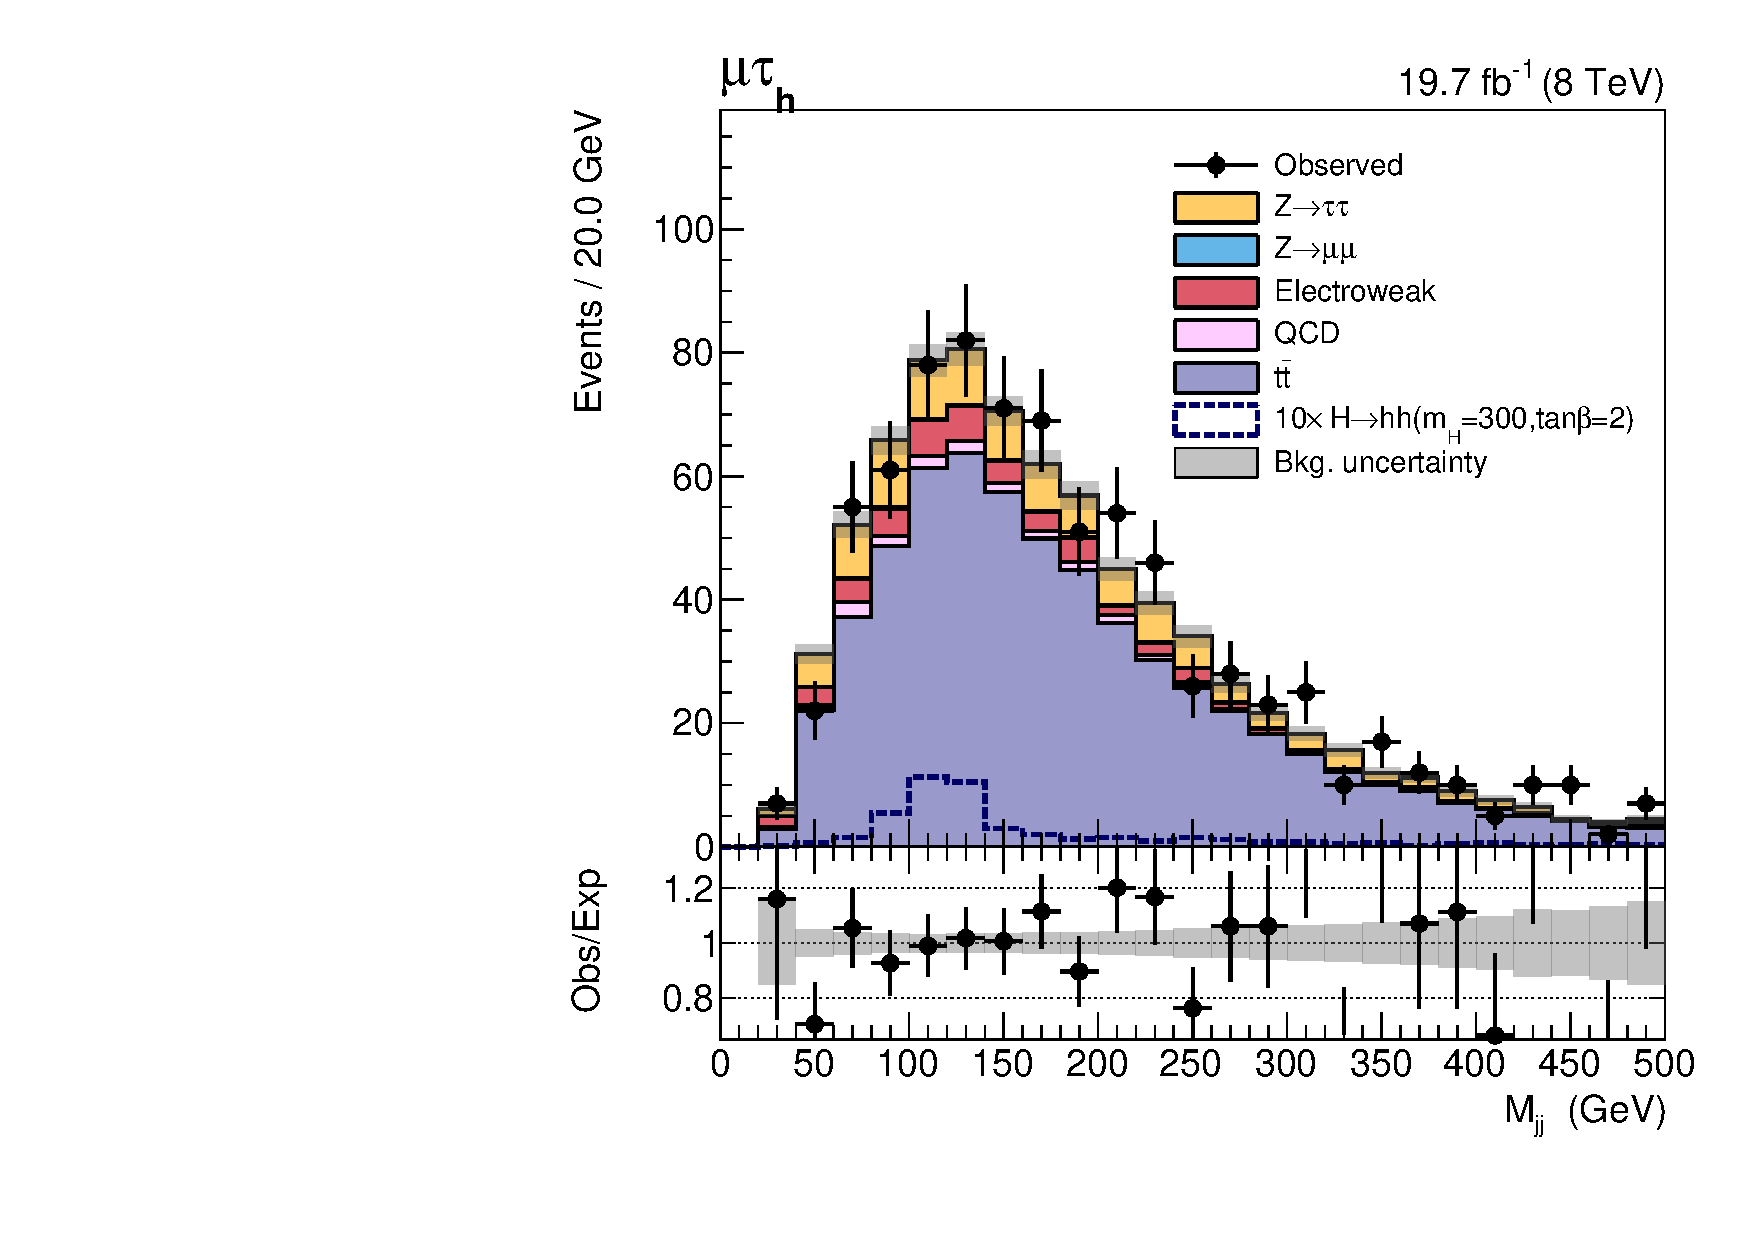
\includegraphics[width=0.5\textwidth]{Hhh/Plots/mjj_2jet2tag_mt_2012.pdf}}
\end{center}
\caption[Reconstruced di-tau invariant mass and di-jet invariant mass in
the 2jet-2tag category of the \mutau channel.]{(a) Reconstructed di-tau invariant mass and (b) di-jet invariant mass in the 2jet-2tag category of the \mutau
channel. The signal for a heavy Higgs boson \PHiggs with mass \mH~$= 300\,\GeV$ at \tanb~$=2$ in the low-\tanb~MSSM scenario, multiplied by a factor 10, is overlaid.
The signal peaks at around $125\,\GeV$ in both variables.}
\label{fig:Hhh_selection_masscuts}
\end{figure}

\section{\acl{MC} simulation to data correction factors}
\label{sec:hhh_datamc}
\ac{MC} samples are used for the estimation of some of the backgrounds and the signal, 
and it is therefore important to correct for any mis-modelling. The \ac{MC} simulation to data 
correction factors used for this are estimated in dedicated control regions.

Identification, isolation, and trigger efficiencies are measured for electrons, muons
and hadronic taus in data and simulated events.
The difference between
the efficiencies in data and simulated events are applied to \ac{MC} events as a
scale factor $\text{SF} = \frac{\epsilon_{\text{Data}}}{\epsilon_{\text{MC}}}$.

For electrons and muons these efficiencies are measured using a 
tag-and-probe method using \Zeenog and \Zmmnog events, respectively.
The hadronic tau identification, isolation and trigger efficiencies
are measured via a similar method that makes use of
$\PZ\rightarrow\Pgt\Pgt\rightarrow\Pgm\Pgth$ events.

The energy scale for hadronic taus is determined by fitting the mass of the 
hadronic tau candidate in $\PZ\rightarrow\Pgt\Pgt\rightarrow\Pgm\Pgth$ events.
This fit is performed separately for each hadronic tau decay mode to obtain
an energy scaling that is applied to reconstructed hadronic taus matched
to simulated hadronic tau decays in \ac{MC} events.

In the \etau channel a scale factor is applied
to the \Zee background to correct for differences in the $\Pe\rightarrow\Pgth$
fake rate between data and simulation. This scale factor is derived separately
for the 1-prong + 0$\pi^0$ and 1-prong + at least one
$\pi^0$ decay modes by fitting the visible mass of the \etau pair
in events passing the selection of the \etau channel as described in section
\ref{sec:hhh_selection_etau}, but with the two-jet requirement removed.

Differences in \MET~resolution and response between data and simulation are accounted for by
applying recoil corrections to \Zellell, \Wjets and signal \ac{MC} events. Section \ref{sec:objects_met_recoilcorr} 
gives more details on how these corrections are derived.

To correct for the differences in b-tagging efficiency and light jet mis-tagging
rates between data and simulation, \pT~and $\eta$~dependent scale factors are 
derived using the method described in reference \cite{BTV8TeV}. There are separate scale factors for 
b-/c-jets and light jets. In this analysis the ``promote/demote'' method
is used to apply these.

In this method a demotion or promotion probability is assigned to every
jet as:
\begin{align}\label{eqn:promotedemote}
&P(\text{demote}) = 1 - \text{SF} \text{  for SF < 1 }  \notag \\
&P(\text{promote}) = \frac{(\text{SF} - 1)(\epsilon_{\text{MC}}-1)}{\text{SF}} \text{    for SF > 1},
\end{align}
Where SF is the scale factor mentioned above, and $\epsilon_{\text{MC}}$ is
the b-tagging efficiency in \ac{MC} events for the type of jet (light, b- or c-)
under consideration.

\section{Discriminating variable}
\label{sec:hhh_discr}
The variable of interest in this analysis is the mass of the heavy Higgs boson \PHiggs. This can be
reconstructed as the four-body mass of the two jets and the two taus. 
A more accurate result can be obtained by using a kinematic fitting 
procedure that makes use of the $125\,\GeV$ mass constraint on the di-tau and
di-jet candidates. 

In a kinematic fit constraints are made on the event kinematics, in the
case of this analysis these constraints are
$m(\Pgt_{1},\Pgt_{2}) = m_{\PHiggslight} = 125\,\GeV$  and
$m(\Pbottom_{1},\Pbottom_{2}) = m_{\PHiggslight} = 125\,\GeV$.
The kinematic observables related to the hadronic taus and jets
are varied within their uncertainties to fulfill these 
constraints. A $\chi^2$ cost term is introduced for each
observable that is varied with respect to the measurement,
the aim of the fit is to minimise the sum of these $\chi^2$ terms.

For b-jets, the reconstructed direction in $\eta$ and $\phi$ is 
assumed to be measured accurately in comparison with their energy.
Therefore only their energy is varied in the fit. In addition, we assume
that uncertainties in the energy measurement directly translate to
uncertainties in the momentum measurement, therefore $\vec{\beta} = \vec{p}/E$ is
also kept constant. 

Before the fit, the mass constraint gives:
~\vspace{-0.5\baselineskip}
\begin{align}\label{eqn:kinfit_prefit}
m_{\PHiggslight}^2 &= E_{\PHiggslight}^2 - \vec{p_{\PHiggslight}}^2 = (E_{\Pbottom 1}+E_{\Pbottom 2})^2 - (\vec{p_{\Pbottom 1}} + \vec{p_{\Pbottom 2}})^2 \notag\\
& = 2E_{\Pbottom 1}E_{\Pbottom 2} + m_{\Pbottom 1}^2 +m_{\Pbottom 2}^2 - 2\vec{p_{\Pbottom 1}}\vec{p_{\Pbottom 2}} \notag\\
& = m_{\Pbottom 1}^2 +m_{\Pbottom 2}^2 - 2E_{\Pbottom 1}E_{\Pbottom 2}(1-\vec{\beta_{\Pbottom 1}}\vec{\beta_{\Pbottom 2}})\notag\\
&\Rightarrow (1-\vec{\beta_{\Pbottom 1}}\vec{\beta_{\Pbottom 2}}) = \frac{m_{\PHiggslight}^2 - m_{\Pbottom 1}^2 - m_{\Pbottom 2}^2}{2E_{\Pbottom 1}E_{\Pbottom 2}}.
\end{align}
When varying the energy of the first jet in the fit, equation \ref{eqn:kinfit_prefit} can be 
rewritten to derive an expression for the updated energy of the second jet. Using $\mathcal{A} = (1-\vec{\beta_{\Pbottom 1}}\vec{\beta_{\Pbottom 2}})$ 
and
~\vspace{-0.5\baselineskip}
\begin{equation}\label{eqn:gamma_def}
\gamma = \frac{1}{1-\beta^2} \Rightarrow \gamma^2 = \frac{1}{1-\beta^2} = \frac{1}{1-p^2/E^2} = \frac{E^2}{m^2},
\end{equation}
we get:
~\vspace{-0.5\baselineskip}
\begin{align}\label{eqn:kinfit_variation}
m_{\PHiggslight}^2 &= m_{\Pbottom 1}^2 + m_{\Pbottom 2}^2 - 2E_{\Pbottom 1}E_{\Pbottom 2}(1-\vec{\beta_{\Pbottom 1}}\vec{\beta_{\Pbottom 2}})\notag\\
&= m_{\Pbottom 1}^2 +\frac{E_{\Pbottom 2,\text{fit}}^2}{\gamma_{\Pbottom 2}^2} +2\mathcal{A}E_{\Pbottom 1}E_{\Pbottom 2,\text{fit}}\notag\\
\Rightarrow E_{\Pbottom 2}^{\text{fit}}& = \frac{(-2E_{\Pbottom 1}\mathcal{A} + \sqrt{4E_{\Pbottom 1}^2\mathcal{A} - 4(m_{\Pbottom 1}^2-m_{\PHiggslight}^2)\gamma_{\Pbottom 2}^{-2}})\gamma_{\Pbottom 2}^2}{2}\notag\\
&= - E_{\Pbottom 1}\mathcal{A}\gamma_{\Pbottom 2}^2+\sqrt{E_{\Pbottom 1}^2\mathcal{A}\gamma_{\Pbottom 2}^4 - (m_{\Pbottom 1}^2 - m_{\PHiggslight}^2)\gamma_{\Pbottom 2}^2}\notag\\
&\Rightarrow E_{\Pbottom 2}^{\text{fit}} = E_{\Pbottom 1}\mathcal{A}\gamma_{\Pbottom 2}^2(-1 + \sqrt{1+\frac{m_{\PHiggslight}^2 - m_{\Pbottom 1}^2}{E_{\Pbottom 1}^2\mathcal{A}\gamma_{\Pbottom 2}^2}}).
\end{align}

The fitting procedure additionally modifies the masses of the b-jets as 
~\vspace{-0.5\baselineskip}
\begin{equation}\label{eqn:kinfit_bjetmass}
m_{\Pbottom_{1,2}}^{\text{fit}} = m_{\Pbottom{1,2}}\frac{E_{\Pbottom{1,2}}^{\text{fit}}}{E_{\Pbottom{1,2}}}.
\end{equation}
The $\chi^2$ term for each b-jet is calculated as $\chi_{\Pbottom 1,2}^2 = \frac{E_{\Pbottom 1,2}^{\text{fit}}-E_{\Pbottom 1,2}^{\text{meas}}}{\sigma_{\Pbottom 1,2}}$.

For taus only the visible decay products are measured. Assuming these point in 
the same direction as the original tau, a similar procedure as for the b-jets can be employed to constrain the energy of the second tau
when varying the energy of the first tau in the fit. The masses of the taus are kept fixed at $m_{\Pgt}$ throughout the procedure.

Due to the missing energy associated with the tau decays, additional constraints
on the fit have to be used to reconstruct the correct tau energies. This is done by 
enforcing that the heavy Higgs boson recoil from the fit is close to the reconstructed recoil.

The measured recoil is 
~\vspace{-0.5\baselineskip}
\begin{equation}\label{eqn:kinfit_recoilmeas}
\vec{p_{\text{T,recoil}}}^{\text{meas}} = -\vec{p_{\text{T,\PHiggs}}}^{\text{meas}} = -\vec{p_{\text{T,miss}}}^{\text{meas}} - \vec{p_{\text{T},\Pbottom 1}}^{\text{meas}} - \vec{p_{\text{T},\Pbottom 2}}^{\text{meas}} - \vec{p_{\text{T},\Pgt_1^{\text{vis}}}}^{\text{meas}} - \vec{p_{\text{T},\Pgt_2^{\text{vis}}}}^{\text{meas}},
\end{equation}
and the recoil from the fit is,
~\vspace{-0.5\baselineskip}
\begin{equation}\label{eqn:kinfit_recoilfit}
\vec{p_{\text{T,recoil}}}^{\text{fit}} = -\vec{p_{\text{T,\PHiggs}}}^{\text{fit}} = - \vec{p_{\text{T},\Pbottom 1}}^{\text{fit}} - \vec{p_{\text{T},\Pbottom 2}}^{\text{fit}} - \vec{p_{\text{T},\Pgt_1}}^{\text{fit}} - \vec{p_{\text{T},\Pgt_2}}^{\text{fit}}.
\end{equation}
A $\chi^2$ corresponding to the agreement between the fitted and measured recoil is reconstructed as
~\vspace{-0.5\baselineskip}
\begin{equation}\label{eqn:kinfit_recoilchi2}
\chi^2_{\text{recoil}} = (\vec{p_{\text{T,recoil}}}^{\text{fit}} - \vec{p_{\text{T,recoil}}}^{\text{meas}})^T V_{\text{recoil}}^{-1}(\vec{p_{\text{T,recoil}}}^{\text{fit}} - \vec{p_{\text{T,recoil}}}^{\text{meas}}),
\end{equation}
where the covariance matrix $V_{\text{recoil}}$ of the recoil vector is estimated as 
\begin{equation}\label{eqn:kinfit_recoilcov}
V_{\text{recoil}} = V_{\vec{p_{\text{T,miss}}}} - V_{\Pbottom {1}} - V_{\Pbottom 2},
\end{equation}
 from the covariance matrices of the b-jets and
the covariance matrix of the missing transverse momentum. The latter is estimated in the process of determining the MVA \MET,
while the covariance matrices of the b-jets can be written in terms of the position, momentum and resolution of the b-jets. 
The total $\chi^2$ term that needs to be minimised in the fit can then be written as
~\vspace{-0.5\baselineskip}
\begin{equation}\label{eqn:kinfit_chitot}
\chi^2 = \chi^2_{\Pbottom 1} + \chi^2_{\Pbottom 2} + \chi^2_{\text{recoil}}.
\end{equation}
The results of the kinematic fit are the tau and b-jet four-vectors with their energies and momenta
set to the best fit values found for them in the fit. These can then be added together to find
the mass of the heavy Higgs boson as reconstructed by the kinematic fit.

As illustrated in figure \ref{fig:kinfitvsmjj}a the use of the kinematic fit greatly
improves the resolution of the reconstructed heavy Higgs boson mass in signal events, when 
compared with the simple four-body mass reconstruction. It also shifts the mean of the
distribution closer to the true value. It is also insightful to make such a comparison
for the \ttbar background, which is the dominant background in the most signal-sensitive categories as 
shown in figure \ref{fig:Hhh_selection_bjets}. This comparison between four-body mass and
kinematic fit mass for \ttbar events is shown in figure 
\ref{fig:kinfitvsmjj}b. From this figure we can see that the mass distribution for
background events is less affected by the kinematic fit, although due to the
invariant mass constraint the minimum of the reconstructed mass distribution
is forced to $250\,\GeV$.

\begin{figure}[h!]
\begin{center}
\subfloat[Signal]{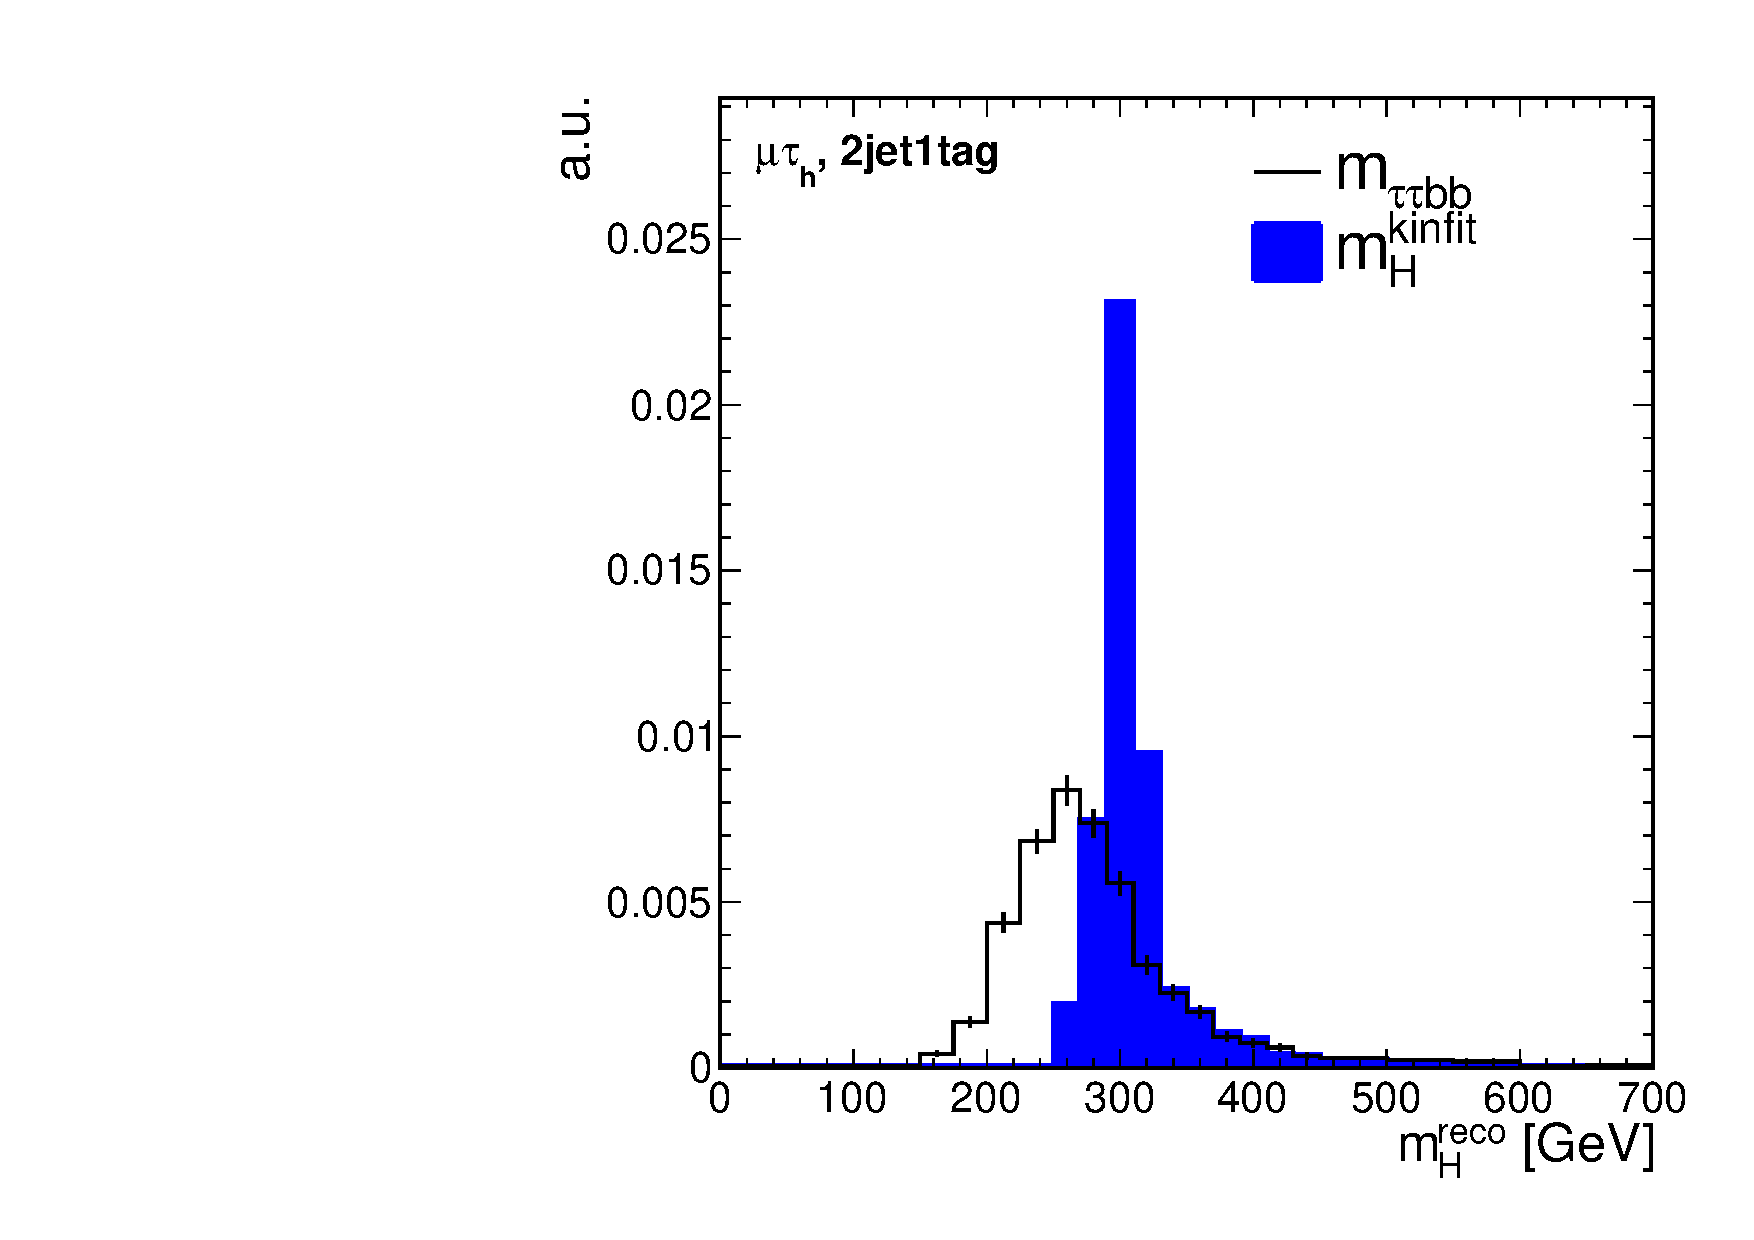
\includegraphics[width=0.5\textwidth]{Hhh/Plots/mHvsmttbb_signal.pdf}}
\subfloat[\ttbar background]{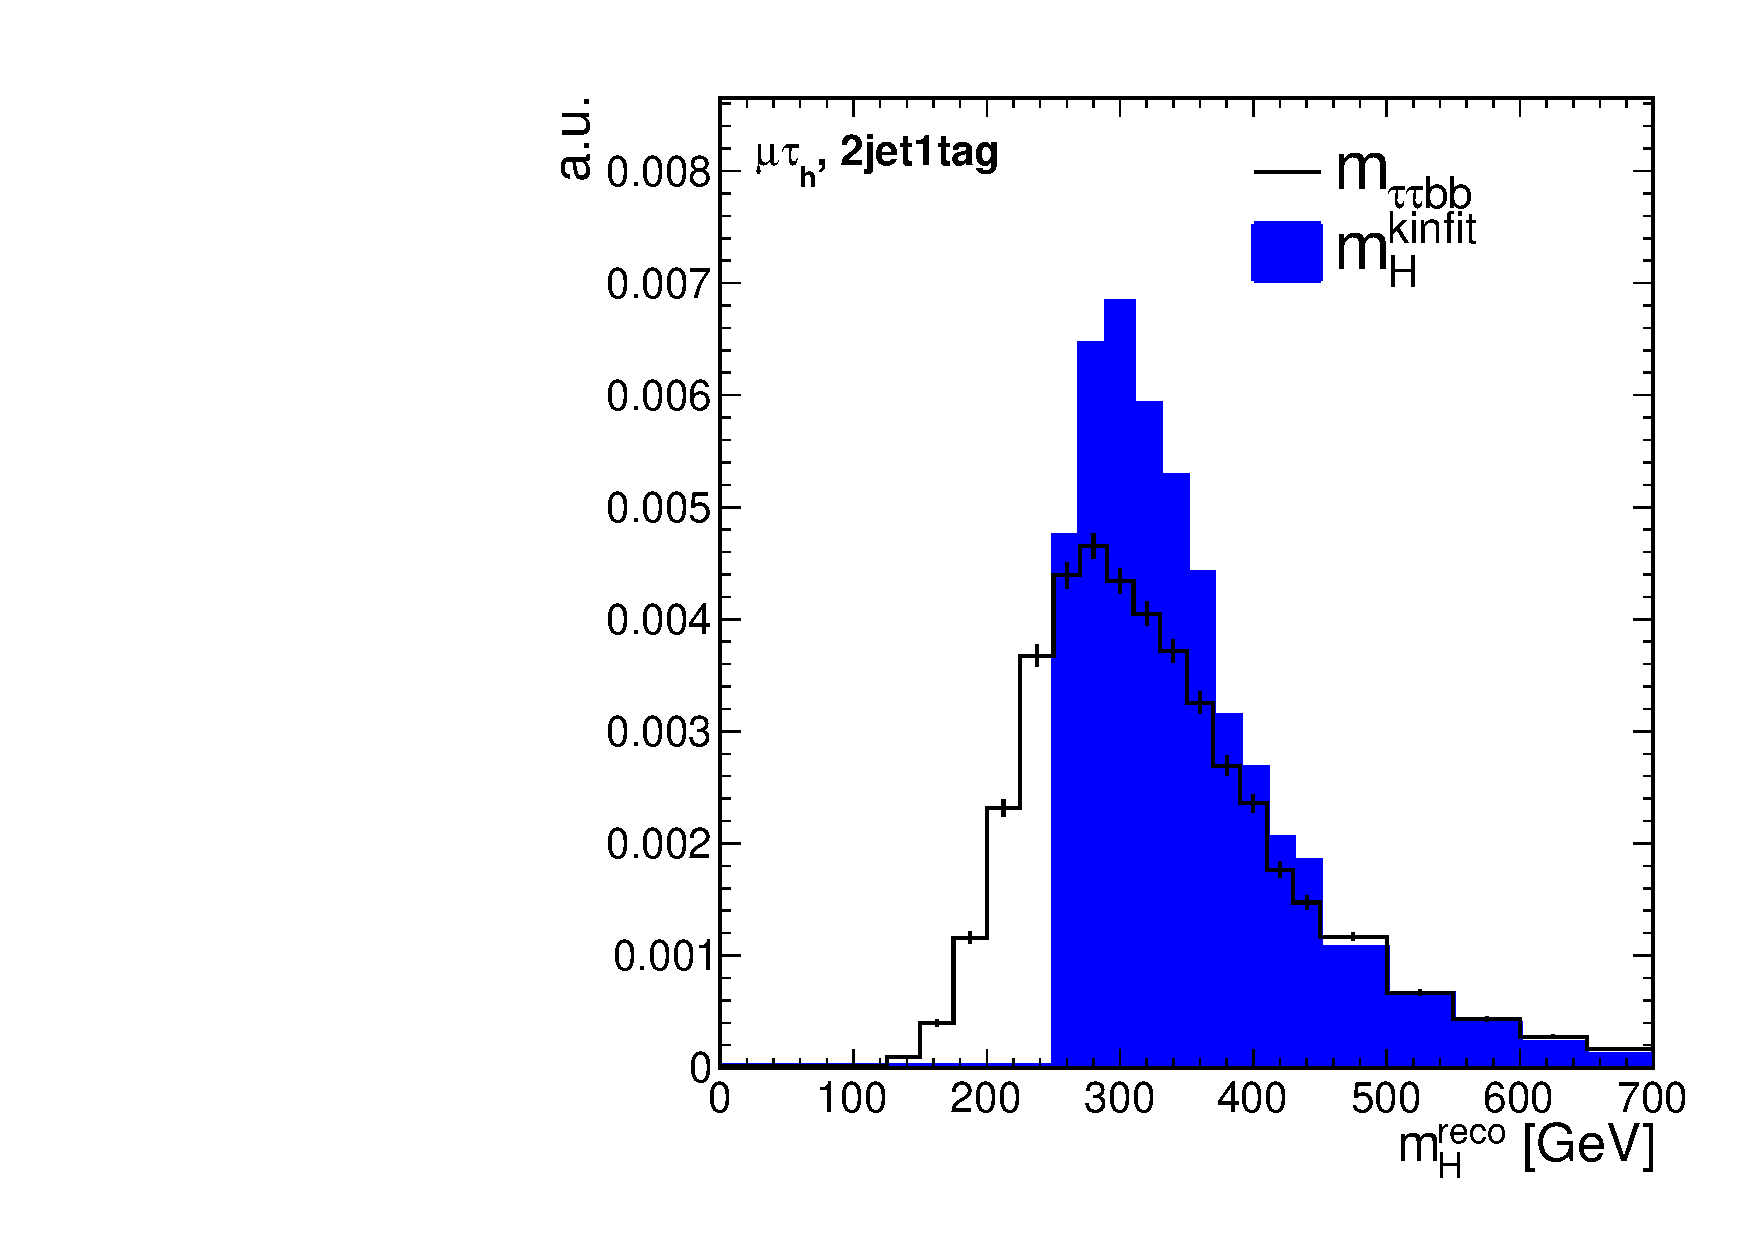
\includegraphics[width=0.5\textwidth]{Hhh/Plots/mHvsmttbb_ttbar.pdf}}
\end{center}
\caption[Comparison of the reconstructed heavy Higgs boson mass
using the kinematic fit in signal events with $m_{\PHiggs}=300\,\GeV$ and \ttbar 
background events in the 2jet-1tag category of the \mutau channel.]{Comparison of the reconstructed heavy Higgs boson mass using the kinematic fit (blue) and
four-body mass without use of the kinematic fit (black) in (a) signal events with $m_{\PHiggs} = 300\,\GeV$ and (b) \ttbar background events in 
the 2jet-1tag category of the \mutau channel. The kinematic fit greatly improves the resolution and 
accuracy of the mean of the mass distribution in signal events.}
\label{fig:kinfitvsmjj}
\end{figure}


\section{Background estimation}
\label{sec:hhh_backgrounds}
To estimate the shape and yield of backgrounds in this analysis, data-driven techniques are
used where possible. 
\subsection{\texorpdfstring{\Ztautau}{Z to tau tau}}
\label{sec:hhh_backgrounds_ztt}
The \Ztautau background is estimated using the embedded samples
described in section \ref{sec:hhh_datasets}. To estimate the 
yield of \Ztautau in each category the total
yield after the initial event selection, before subdividing into categories, as
estimated in the \Ztautau \ac{MC} sample is scaled by the efficiency with which 
such events pass the category selection in the embedded sample. The shape of
the \Ztautau background is taken from the embedded sample after applying the full
category selection. The contamination from the \ttbar background in the embedded
sample is evaluated using the dedicated \ttbar embedded sample. This contribution
is subtracted from the \Ztautau background.
\subsection{\texorpdfstring{\ttbar}{ttbar}}
Both the \ttbar shape and normalisation are estimated using \ac{MC} samples.
These are checked against data in dedicated control regions. One such control
region uses the \emu final state of the di-tau pair. A correction factor is estimated in 
this control region and applied to the yield estimate from simulation in the signal region. 
%The resulting scale factor is 1.033 ± 0.013(stat.) ± 0.088(syst.). 
\subsection{\texorpdfstring{\Wjets}{W + jets}}
\label{sec:hhh_backgrounds_wjets}
The \Wjets background is greatly reduced by requiring \mT~to
be less than $30\,\GeV$. To estimate the remaining contribution
in the signal region a sideband with \mT~greater
than $70\,\GeV$ is used in the 2jet-0tag and 2jet-1tag categories.
Contributions from other backgrounds are subtracted 
from the data in this region, and a high-\mT~to low-\mT~extrapolation
 factor is determined from the \Wjets \ac{MC} 
sample. The yield in the signal region is given by the data yield in the high-\mT~sideband, with
other backgrounds subtracted, multiplied by this extrapolation factor.
In the 2jet-2tag category, a slightly different high-\mT~sideband of $60$--$120\,\GeV$ is used 
as above $120\,\GeV$ the \ttbar background dominates over \Wjets. 
The method of extrapolating this yield estimate into
the signal region is otherwise analogous.

The shape of the \Wjets distribution is taken from the simulation. To 
increase the number of events for this estimate, the b-tagging definition
in the 2jet-1tag and 2jet-2tag categories is relaxed from the medium to the loose 
working point for the purposes of shape estimation.
\subsection{QCD multijet}
\label{sec:hhh_backgrounds_qcd}
A fully data-driven method is used to estimate the QCD background. Here, di-tau candidates
of the same sign, which otherwise pass the signal region selection, are used. 
The contributions from other backgrounds
in this same-sign (SS) region are subtracted from the number of data events obtained.
As the contributions from opposite-sign (OS) and same-sign QCD are
not exactly the same an OS/SS ratio is applied to the same-sign region data yield with other backgrounds subtracted.
The OS/SS ratio is measured using data with 
the electron or muon isolation requirements inverted. 

For the 2jet-0tag and 2jet-1tag categories the yield is taken directly from
the same-sign subtracted data multiplied by the OS/SS ratio. In the 2jet-2tag
category the number of available events is too low for this, so another sideband is defined
in which the electron or muon isolation requirement is inverted. This 
sideband is then used to determine an extrapolation factor from events
with two jets to events passing the 2jet-2tag category selection. This extrapolation
factor is then applied to a QCD estimate as described above, but using the two-jet 
selection only, to obtain the yield in the 2jet-2tag category.

The shapes in all categories are taken from same-sign data with the electron or muon
isolation inverted. For the 2jet-1tag and 2jet-2tag categories, in addition to 
inverting the light lepton isolation requirements, the category definition
is relaxed to obtain the shapes. For the purposes of QCD shape
estimation, jets are considered b-tagged if they pass the loose b-tagging
working point.
\subsection{Other backgrounds}
\label{sec:hhh_backgrounds_other}
The remaining backgrounds of \Zellell, di-boson and single-top
events are small. Both shapes and normalisations are
estimated using \ac{MC} samples.
 
\section{Systematic uncertainties}
\label{sec:hhh_uncs}
Two types of systematic uncertainties are considered: normalisation
uncertainties and shape uncertainties. Normalisation uncertainties affect only
the yield of a process, while shape uncertainties affect both the yield of a process and the 
shape of its kinematic fit mass distribution. 
Section \ref{sec:hhh_results_extraction}
describes how these uncertainties are taken into account in the final result.
\subsection{Normalisation uncertainties}
\label{sec:hhh_uncs_norm}
\subsubsection*{Luminosity uncertainty}
The uncertainty on the luminosity measurement amounts to 2.6\% \cite{CMS-PAS-LUM-13-001} for data collected during
2012. This uncertainty is applied to all processes in which
the normalisation is estimated using simulation.
\subsubsection*{Identification, isolation and trigger efficiencies}
A systematic uncertainty on the efficiency measurements
for the leptons is derived by combining the separate uncertainties on these measurements
in quadrature. For electrons and muons this leads to a 2\% uncertainty. For hadronic taus a 6\% 
uncertainty is measured on the tau identification efficiency, with an additional uncertainty of 3\% for
the tau legs of the triggers \cite{CMS-HIG-14-034}. The identification, isolation and trigger efficiency measurement uncertainties are applied to all processes for which
the normalisation is estimated using simulation.
\subsubsection*{$\Pe\rightarrow\Pgth$ and $\Pgm\rightarrow\Pgth$ fake rates}
The uncertainty on both the $\Pe\rightarrow\Pgth$ fake rate measurement and the
$\Pgm\rightarrow\Pgth$ fake rate measurement is 30\% \cite{SMHtautauCMS}. The central value of the $\Pgm\rightarrow\Pgth$
fake rate correction is close to 1, which is why it is not applied, but the uncertainty is 
taken into account.
\subsubsection*{b-Tag scale factors}
The b-tag scale factors are varied within their uncertainties, as described in reference \cite{cms-btag-paper}, to determine the effect
on the yields of each process. Both a b-tagging uncertainty and a light jet mis-tagging
uncertainty are obtained by considering the percentage by which these backgrounds
change when the scale factors are varied within their uncertainty. The b-tagging
efficiency uncertainty amounts to $1$--$10$\% for most processes in most categories, except for the 2jet-2tag
category where a 70\% uncertainty applies to the \Wjets background. 
This uncertainty is large because in this category there is a significant amount of \ttbar in the 
control region used for the \Wjets estimate. A 10\% change in the \ttbar yield causes the \Wjets
yield to vary by this amount.
The light jet mis-tagging rate uncertainty varies between $1$--$5$\% for all processes in all channels.
\subsubsection*{\MET~resolution and response}
Uncertainties on the \MET~resolution and response are estimated by varying
the recoil correction parameters within their estimated uncertainties. This 
leads to a $1$--$10$\% uncertainty, depending on the category and process considered.
\subsubsection*{Background normalisation}
\begin{itemize}
\item \Ztautau : The inclusive normalisation of the embedded samples has a 3.3\% uncertainty, which is derived
from combining the estimated normalisation uncertainty on the embedded samples themselves, and the uncertainty on the \ttbar embedded samples. In addition, an uncertainty of $5$--$6$\% for extrapolation from the inclusive selection to the category selection is applied.
\item \Zellell: As this is a very small background after requiring two jets, the uncertainty on this estimate is derived from the statistical uncertainty on the yield estimate, which varies between $20$--$90$\%.
\item \ttbar: The uncertainty on the \ttbar cross section is 10\% \cite{SMHtautauCMS}.
\item Di-boson and single top: The combined uncertainty on the di-boson and single-top cross sections is 15\% \cite{SMHtautauCMS}.
\item \Wjets: As the \Wjets yield is estimated from a high \mT~sideband in data, the uncertainty on this yield estimate is primarily due to the number of events available in the control region. The uncertainty ranges from 10\% in the 2jet-0tag category to 100\% in the 2jet-2tag category.
\item QCD: The QCD normalisation uncertainty is obtained by adding the statistical uncertainty on the data-subtracted same-sign region in quadrature with the 10\% uncertainty on the OS/SS ratio. This yields a 20\% uncertainty in the 2jet-0tag category, a 40\% uncertainty in the 2jet-1tag category and a $60$--$100$\% uncertainty in the 2jet-2tag category.
\end{itemize}
\subsection{Shape uncertainties}
\label{sec:hhh_uncerts_shape}
\subsubsection*{Tau energy scale}
The energy of hadronically decaying taus is varied up and down by a 3\% uncertainty \cite{SMHtautauCMS}. As this directly affects the kinematic fit mass distribution this uncertainty is then applied as a shape uncertainty.
\subsubsection*{Jet energy scale}
The uncertainties on the jet energy corrections are applied by shifting the jet energy up and down by the \pT-and $\eta$-dependent uncertainty \cite{cms-jec-2011}. Again, as this affects the shape of the kinematic fit mass distribution this uncertainty is applied as a shape uncertainty.
\section{\texorpdfstring{Overview of \AtoZhtolltautau}{Overview of A->Zh->lltautau}}
\label{sec:hhh_azh}
In this section a summary of the \AtoZhtolltautau analysis \cite{CMS-HIG-14-034}, which is combined with the 
analysis described so far for the purpose of model interpretations, is given.

The search for \AtoZhtolltautau also uses the full dataset collected by the CMS experiment during
the 2012 p-p running period of the \ac{LHC}. In this search the \mumu and \ee final states of the \PZ boson
and the \emu, \etau, \mutau and \tautau channels of the \htotautau decay are considered, leading to a total of
eight final states. 

First the \PZ candidate is chosen as a pair of isolated electrons or muons, with opposite charge, and 
invariant mass between $60$--$120\,\GeV$. If there is more than one possible pair, the 
pair with invariant mass closest to the \PZ boson mass is chosen. The \htotautau decay is chosen by selecting
an oppositely charged pair of isolated particles in the four channels mentioned above. To ensure no overlap
between different final states is possible, events with additional electrons or muons satisfying the
\pT~and $\eta$ requirements are discarded.

To reject some of the backgrounds from misidentified leptons and \ZZ production, a requirement is made
on the scalar sum of the visible transverse momenta of the two tau candidates from the \htotautau decay.
This selection changes by final state and has been chosen to optimise the analysis sensitivity to an 
\AtoZh signal with \mA~$= 220$--$350\,\GeV$. Furthermore, \ttbar events are discarded by rejecting
events with at least one b-tagged jet. 

Remaining backgrounds from \ZZ, tri-boson and \ttbar+\PZ production are estimated using
simulation. Backgrounds from $\PZ+$jets %($\ell\ell\tautau$ channel) 
and $\WZ+$jets %($\ell\ell\mutau$ and $\ell\ell\etau$ channels) 
events, with at least one misidentified lepton, are estimated from control regions in data.

For signal extraction the mass of the \PHiggsps boson, \mA, is used. This mass is reconstructed by combining the
four-vector of the \PZ boson candidate with the four-vector of the \PHiggslight candidate as obtained by using the 
\texttt{SVFit} algorithm. The expected and observed 95\% \ac{CL} upper limits, for
all $\ell\ell\tau\tau$ final states combined, is shown in figure \ref{fig:AZhUpperLimits}.

\begin{figure}[h!]
\begin{center}
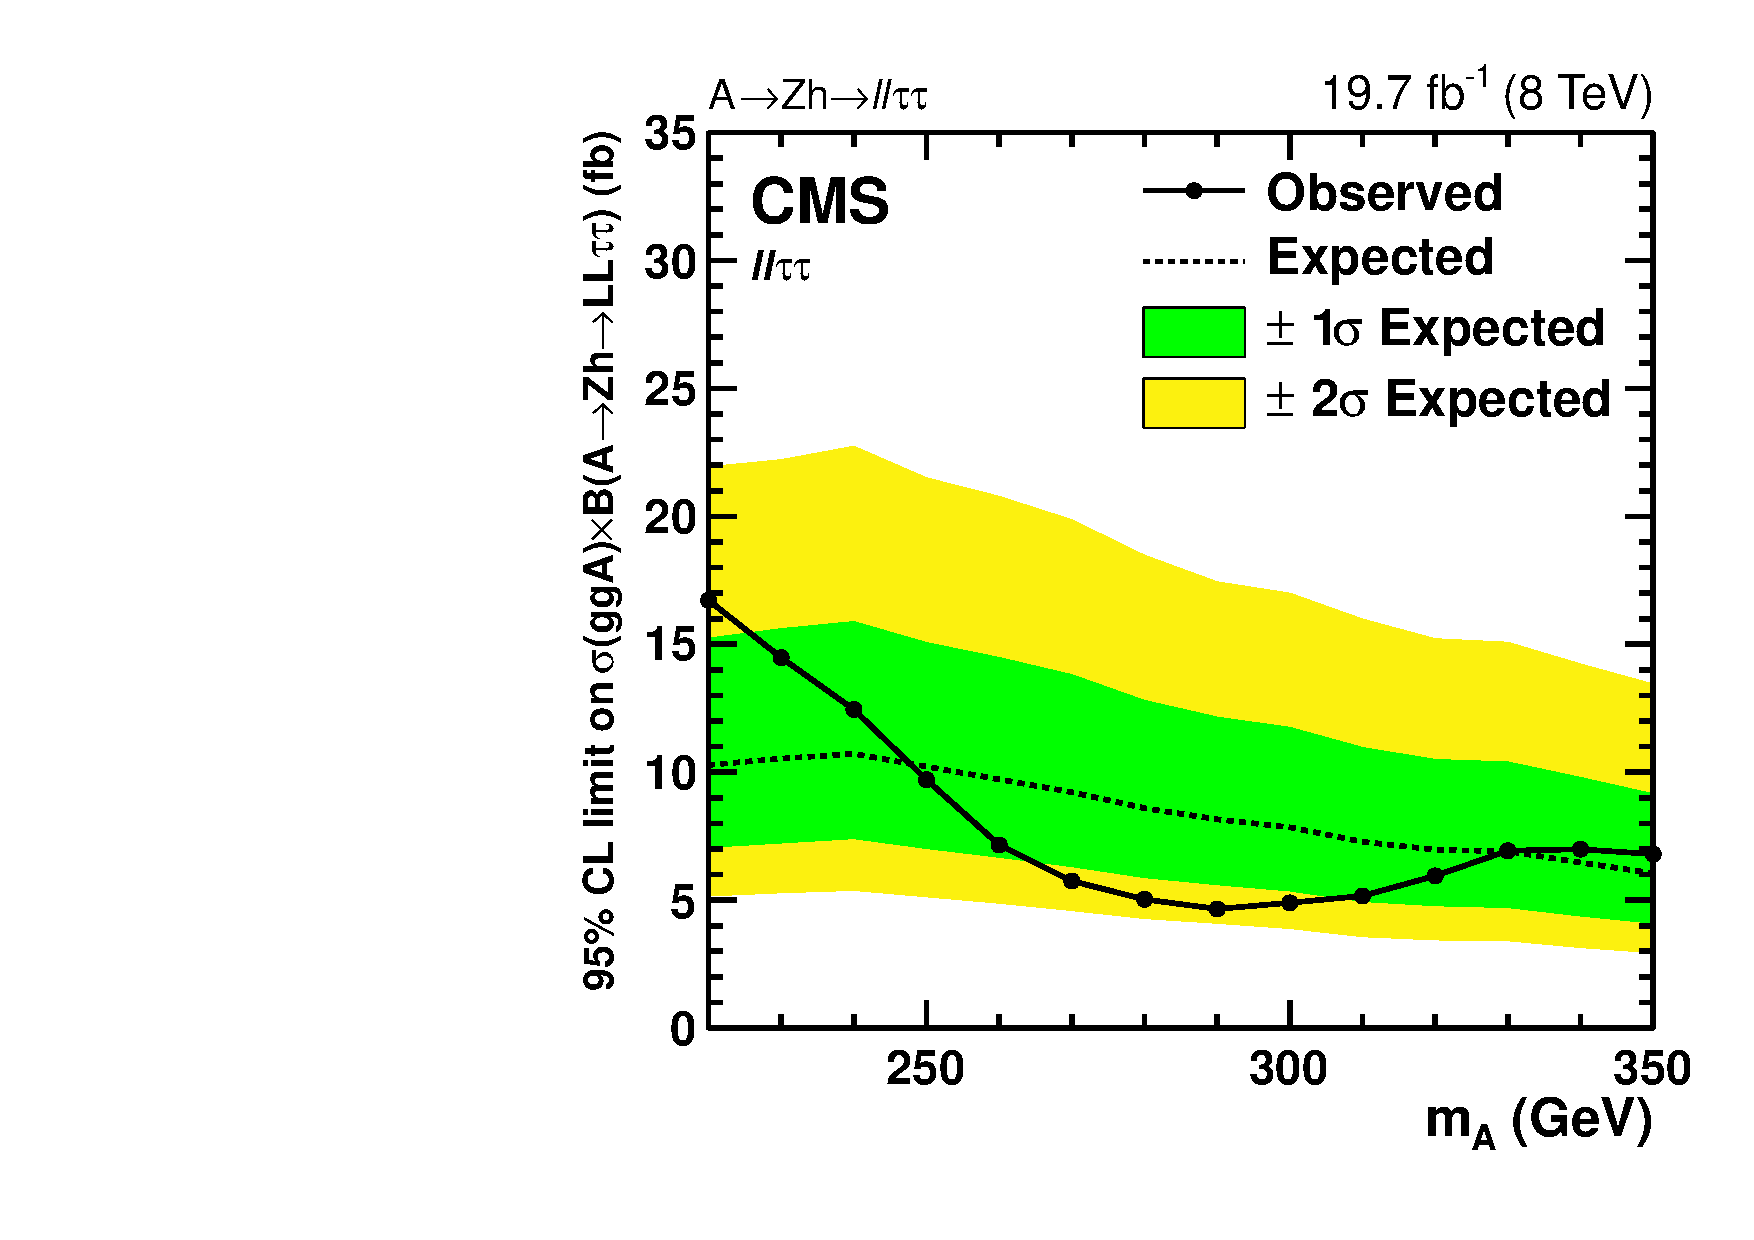
\includegraphics[width=0.5\textwidth]{Hhh/Plots/CMS-HIG-14-034_Figure_010-a.pdf}
\caption[The 95\% confidence level expected and observed upper limits on the 
\xsbr for the \AtoZhtolltautau process.]{The 95\% confidence level expected (dashed) and observed (solid)
upper limits on the \xsbr for the \AtoZhtolltautau process.
The green and yellow bands indicate the $\pm 1 \sigma $ and $\pm 2\sigma$
expectations \cite{CMS-HIG-14-034}.}
\label{fig:AZhUpperLimits}
\end{center}
\end{figure}

More detail on this analysis can be found in reference \cite{CMS-HIG-14-034}.
Systematic uncertainties are also applied in the \AtoZhtolltautau analysis. 
For the purpose of combining the results with the \Htohhtobbtautau search,
some of these are correlated between the two analyses.
This applies to the
luminosity uncertainty and the uncertainties on b-tagging efficiency
and light jet mis-tagging rate.

\section{Results}
\label{sec:hhh_results}
\subsection{Signal extraction}
\label{sec:hhh_results_extraction}
The kinematic fit mass $m_{\PHiggs}^{\text{kinfit}}$ is used as the discriminating variable in the \Htohh analysis.
For each channel and category the compatibility of the $m_{\PHiggs}^{\text{kinfit}}$ distribution
of the observed data with the expected background distribution can be assessed. All bins
of the $m_{\PHiggs}^{\text{kinfit}}$ distribution are used to perform a shape analysis. The 
statistical methods used are recommended by the LHC Higgs Combination Group \cite{LHCHComb2011} 
and are used for all Higgs analyses in ATLAS and CMS. 

The likelihood function for data, whether observed or pseudo-data, is constructed as 
\begin{equation} \label{eqn:hhh_likelihood}
\mathcal{L}(\text{data}|\mu, \theta) = \Sigma_i\text{Poisson}(n_{i}|(\mu\cdot s_i(\theta) + b_i(\theta)) )\cdot p(\tilde{\theta}|\theta),
\end{equation}
where $\text{Poisson}(n_{i}|(\mu\cdot s_i(\theta)+b_i(\theta)))$ is given by
\begin{equation}\label{eqn:hhh_poisson}
\text{Poisson}(n_{i}|(\mu\cdot s_i(\theta)+b_i(\theta))) = \frac{(\mu\cdot s_i(\theta) + b_i(\theta))^{n_i})}{n_i!}e^{-(\mu\cdot s_i(\theta)+b_i(\theta))},
\end{equation}
with $n_i$ the number of 
data events in bin $i$.

The first term in equation \ref{eqn:hhh_likelihood} integrates over all bins of the $m_{\PHiggs}^{\text{kinfit}}$ distribution 
in all channels and categories. The parameter $s$ represents the number of expected signal events
in each bin, and $b$ the number of expected background events. These are functions of 
$\theta$, the full set of nuisance parameters. The signal strength
modifier $\mu$ can represent different quantities depending on the normalisation of the 
signal expectation. In the case of the \Htohhtobbtautau analysis the signal is normalised
to $1\,\picobarn$, so the signal strength modifier represents
the \xsbr of a possible signal.

The second term in equation \ref{eqn:hhh_likelihood}, $p(\tilde{\theta}|\theta)$ represents the full set of 
probability density functions of the uncertainties on the nominal
values of the nuisance parameters $\tilde{\theta}$. Each nuisance parameter represents a systematic uncertainty
as discussed in section \ref{sec:hhh_uncs}. The functional form of the probability density function
depends on the type of systematic uncertainty. Normalisation uncertainties are applied with log-normal constraints, which
ensures that the process yields can never become negative, and therefore unphysical, in the fit. 
%For a log-normal constraint an $n~\sigma$ upwards pull on a nuisance parameter $\theta$ measured with a systematic
%uncertainty $\kappa$ multiplies the yield of processes affected by this nuisance parameter by $(1+\kappa)^n$, while
%an $n~\sigma$ downwards pull multiplies the process yields by $(1+\kappa)^{-n}$, ensuring that process
%yields do not become negative. 
Shape uncertainties are accounted for using a vertical template morphing
technique \cite{temp-morph-2011}. For each nuisance parameter that affects the shape of the fitted distribution, two additional
templates corresponding to the quantity varied by $\pm 1 \sigma$ are generated. A nuisance
parameter is added to the likelihood model with a gaussian constraint to smoothly interpolate between
the nominal and $\pm 1\sigma$ templates. Limitations in the number of events used to construct the shape templates
are accounted for by the Barlow-Beeston method\cite{BarlowBeeston}, in which each of the bins of each 
shape template is allowed to vary within its statistical uncertainty, independent of the other bins. %These
%variations are controlled by log-normal constraints in the likelihood function.

To compare the data with the background-only and signal-plus-background hypotheses, a test
statistic $q_{\mu}$ can be defined. This is a single 
number that is used to distinguish between the two hypotheses. The test
statistic used for LHC Higgs analyses, known as the profile likelihood, is given 
by
\begin{equation}\label{eqn:hhh_profilelikelihood}
q_{\mu} = -2\text{ln}\frac{\mathcal{L}(\text{data}|\mu,\hat{\theta_{\mu}})}{\mathcal{L}(\text{data}|\hat{\mu},\hat{\theta})},
\end{equation}

where $0 \leq \hat{\mu} \leq \mu$ is required for setting upper limits.

In this equation $\mu$ is the signal strength modifier being tested, $\hat{\theta_{\mu}}$ denotes the values of the
nuisance parameters which maximise the likelihood for that particular $\mu$, while $\hat{\mu}$ and $\hat{\theta}$ are
the values of the signal strength modifier and the nuisance parameters which give the global maximum of the likelihood.
The requirements on $\mu$ ensure that the signal strength is non-negative and that
a one-sided confidence interval is constructed so as not to allow the observation of  a 
signal with strength $\hat{\mu} > \mu$ to cause rejection of the signal hypothesis.

The probabilities of finding a value $q_{\mu}$ at least as large as the observed value $q_{\mu}^{\text{obs}}$, assuming the signal-plus-background hypothesis
and assuming the background-only hypothesis, are given by

\begin{equation}\label{eqn:hhh_pvaluesig}
p_{\mu} = P(q_{\mu} \geq q_{\mu}^{\text{obs}} | \text{s+b}) = \int_{q_{\mu}^{\text{obs}}}^{\infty} f(q_{\mu} | \mu,\hat{\theta_{\mu}^{\text{obs}}}) dq_{\mu},
\end{equation}

and 
\begin{equation}\label{eqn:hhh_pvaluebkg}
1-p_b = P(q_{\mu} \geq q_{\mu}^{\text{obs}} | \text{b}) = \int_{q_{0}^{\text{obs}}}^{\infty} f(q_{\mu} | 0,\hat{\theta_{0}^{\text{obs}}}) dq_{\mu} ,
\end{equation}

where $f(q_{\mu}|\mu,\hat{\theta_{\mu}})$ and $f(q_{\mu} | 0,\hat{\theta_0})$ are the probability density functions of $q_{\mu}$ under
the signal-plus-background and background-only hypotheses.

Using this, $\text{CL}_s$ is defined as
\begin{equation}\label{eqn:hhh_cls}
\text{CL}_s(\mu) = \frac{\text{CL}_{s+b}}{\text{CL}_b} = \frac{p_{\mu}}{1-p_b}.
\end{equation}

The value of $\mu$ for which $\text{CL}_s$ equals $\alpha$ is referred to as the upper limit on $\mu$ at
\acf{CL} $1-\alpha$. Upper limits at the LHC are generally
quoted at 95\% \ac{CL}. %, therefore the upper limit on cross-section times branching ratio
%for the \Htohhtobbtautau process at this level is obtained as the value of $\mu$ for which $CL_s$ 
%equals 0.05. The use of $CL_s$ to set
The use of $\text{CL}_s$ to set exclusion limits is referred to as the modified frequentist approach\cite{CLS}.

The distributions $f(q_{\mu}|\mu,\hat{\theta_{\mu}})$ and $f(q_{\mu}|0,\hat{\theta_0})$ are determined
using toy MC datasets. These datasets are generated from the signal-plus-background or background-only expectations respectively. 
To generate each toy dataset the nuisance parameters are fixed to their best-fit values as found in the fit to the observed data.
The number of events in each bin in the toy dataset is set using poisson fluctuations around the expectation in that bin, and the effect of
systematic uncertainties is taken into account by sampling a set of pseudo measurements $\tilde{\theta}'$ for each toy, based on the 
probability density function $p(\tilde{\theta}|\theta)$.
The probability density function of $q_{\mu}$ under the relevant hypothesis (signal-plus-background or background-only)
can by found be accumulating a large number of toy datasets and evaluating $q_{\mu}$ for each of them.

This method of generating toy MC datasets can be computationally intensive.
In the limit of a large number of events $f(q_{\mu})$ follows a known formula \cite{AsymptoticFormula}.
This formula, known as the asymptotic approximation, allows for the calculation
of the observed limit as well as the median and $\pm 1\sigma$ and $\pm 2\sigma$ expected limits using
the properties of the Asimov dataset: a dataset in which the observation in 
each bin exactly matches the predictions of the model. This method is used for the analysis
described in this chapter, removing the need to generate toy datasets.

\subsection{Model-independent results}
\label{sec:hhh_results_modelindep}

The $m_{\PHiggs}^{\text{kinfit}}$ distributions in all categories of the \mutau and \etau channels, after the fit to the
observed data has been performed, are shown in figures \ref{fig:hhh_results_mhkinfit_mutau} and \ref{fig:hhh_results_mhkinfit_etau} 
respectively.

\begin{figure}[h!]
\begin{center}
\subfloat[2jet-0tag]{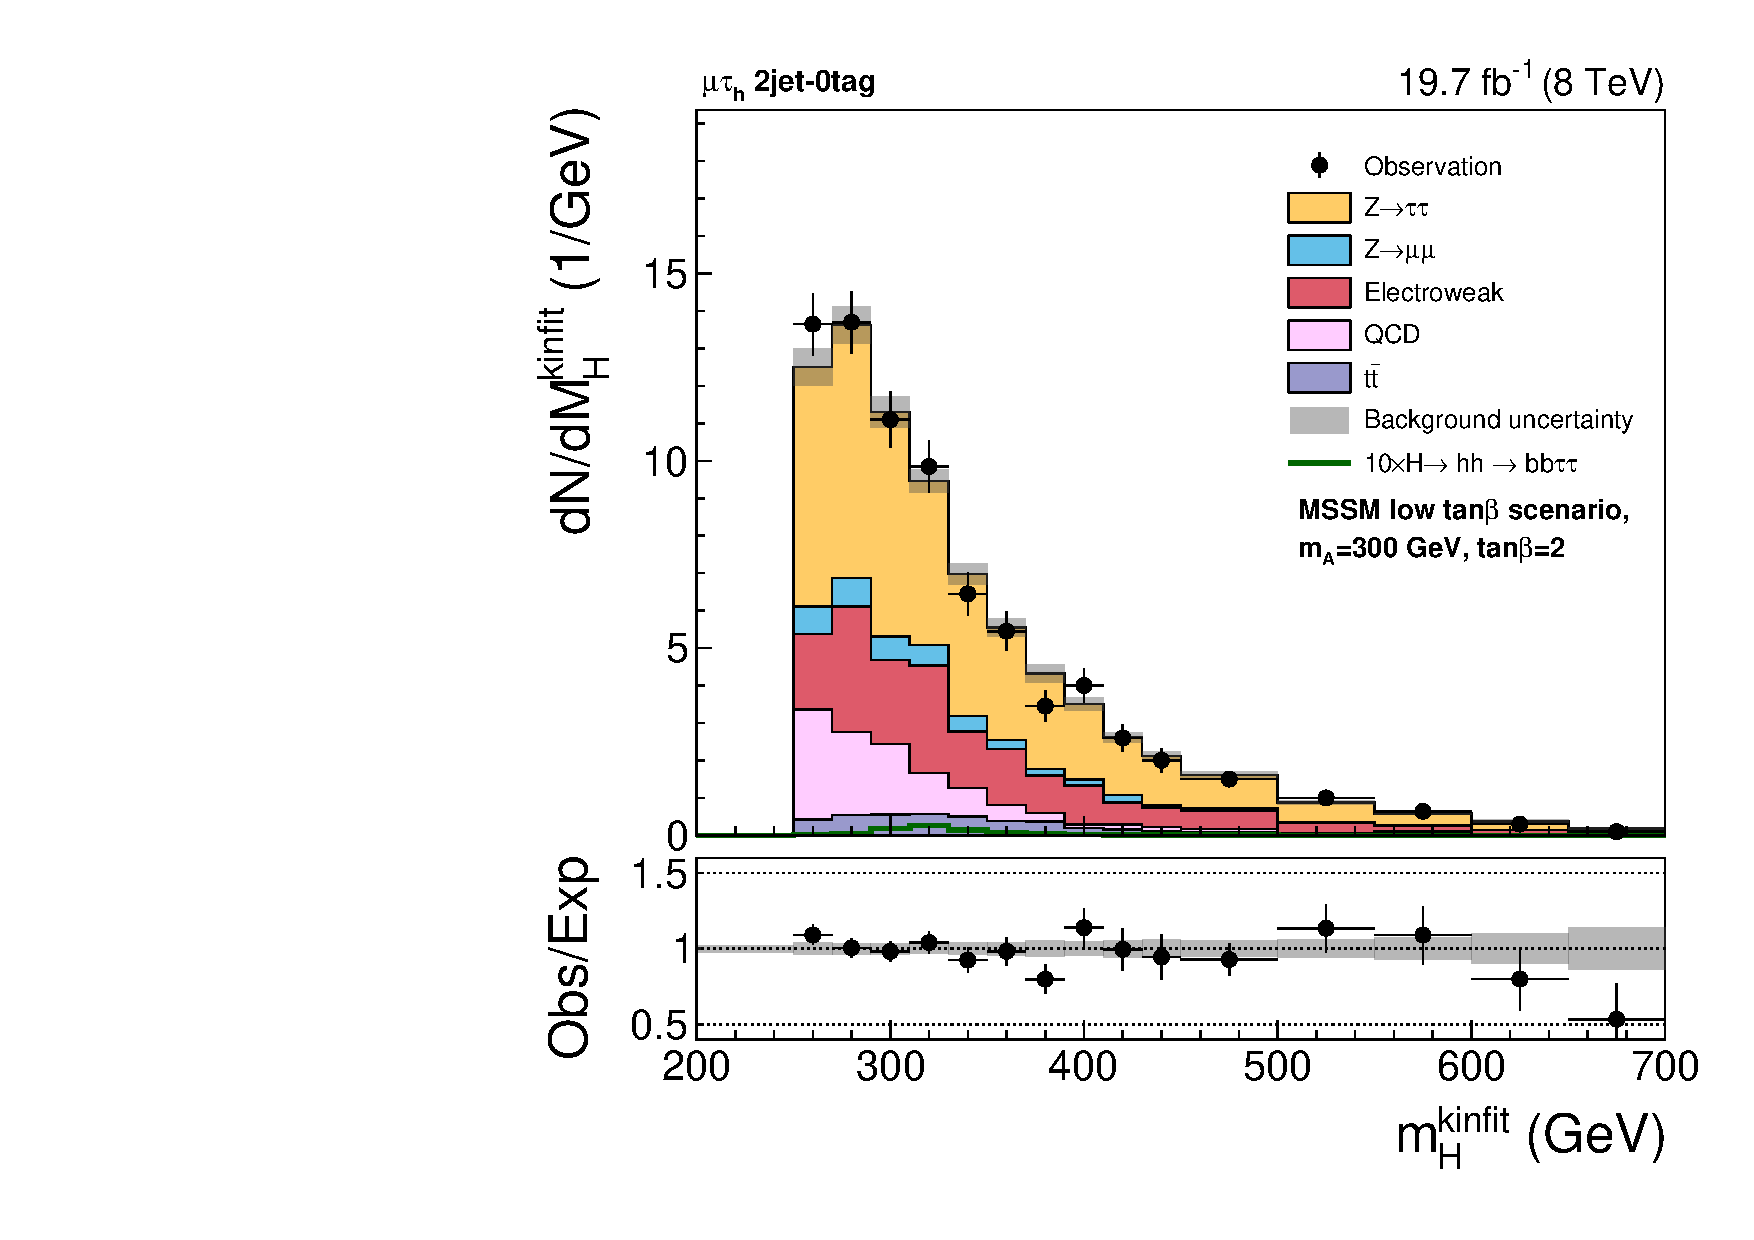
\includegraphics[width=0.5\textwidth]{Hhh/Plots/htt_mt_0_shapes_postfit.pdf}}
\subfloat[2jet-1tag]{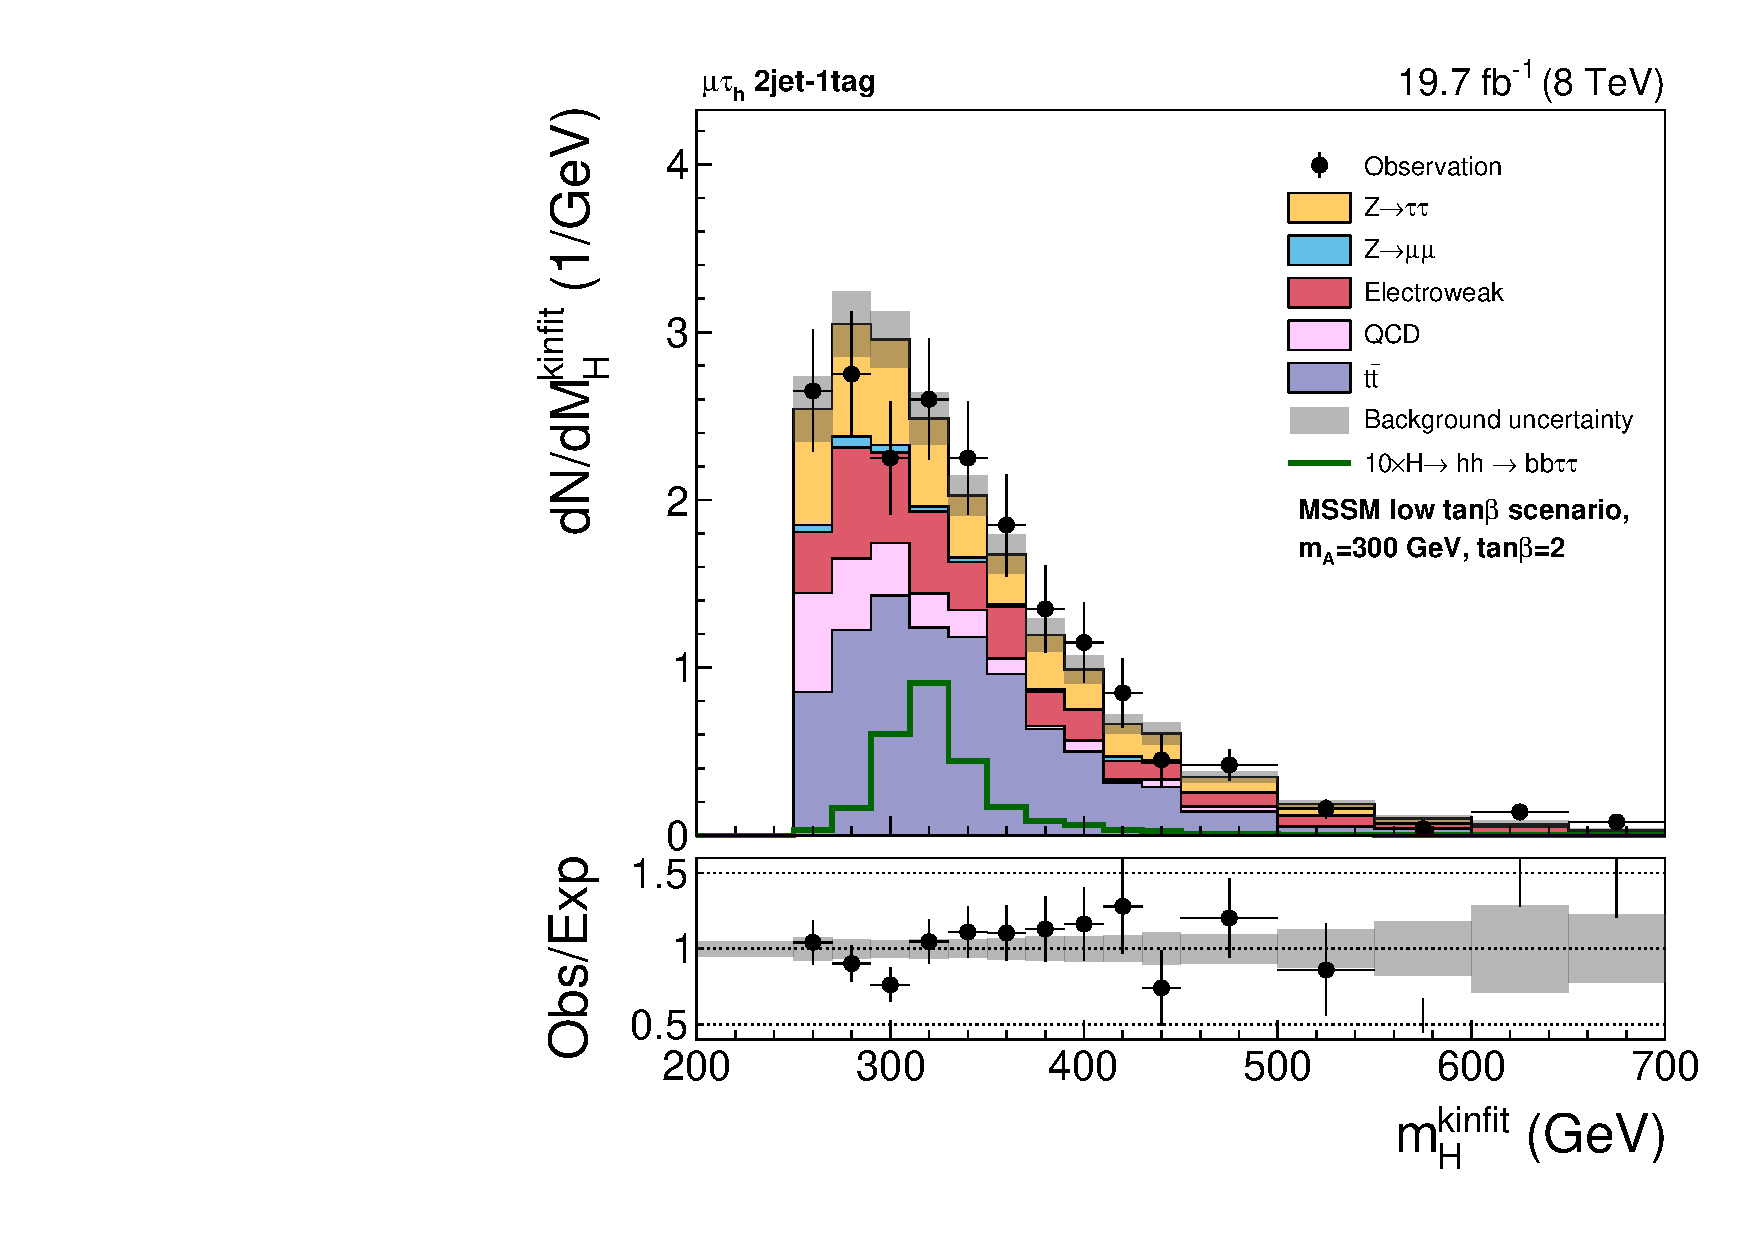
\includegraphics[width=0.5\textwidth]{Hhh/Plots/htt_mt_1_shapes_postfit.pdf}}~\\
\subfloat[2jet-2tag]{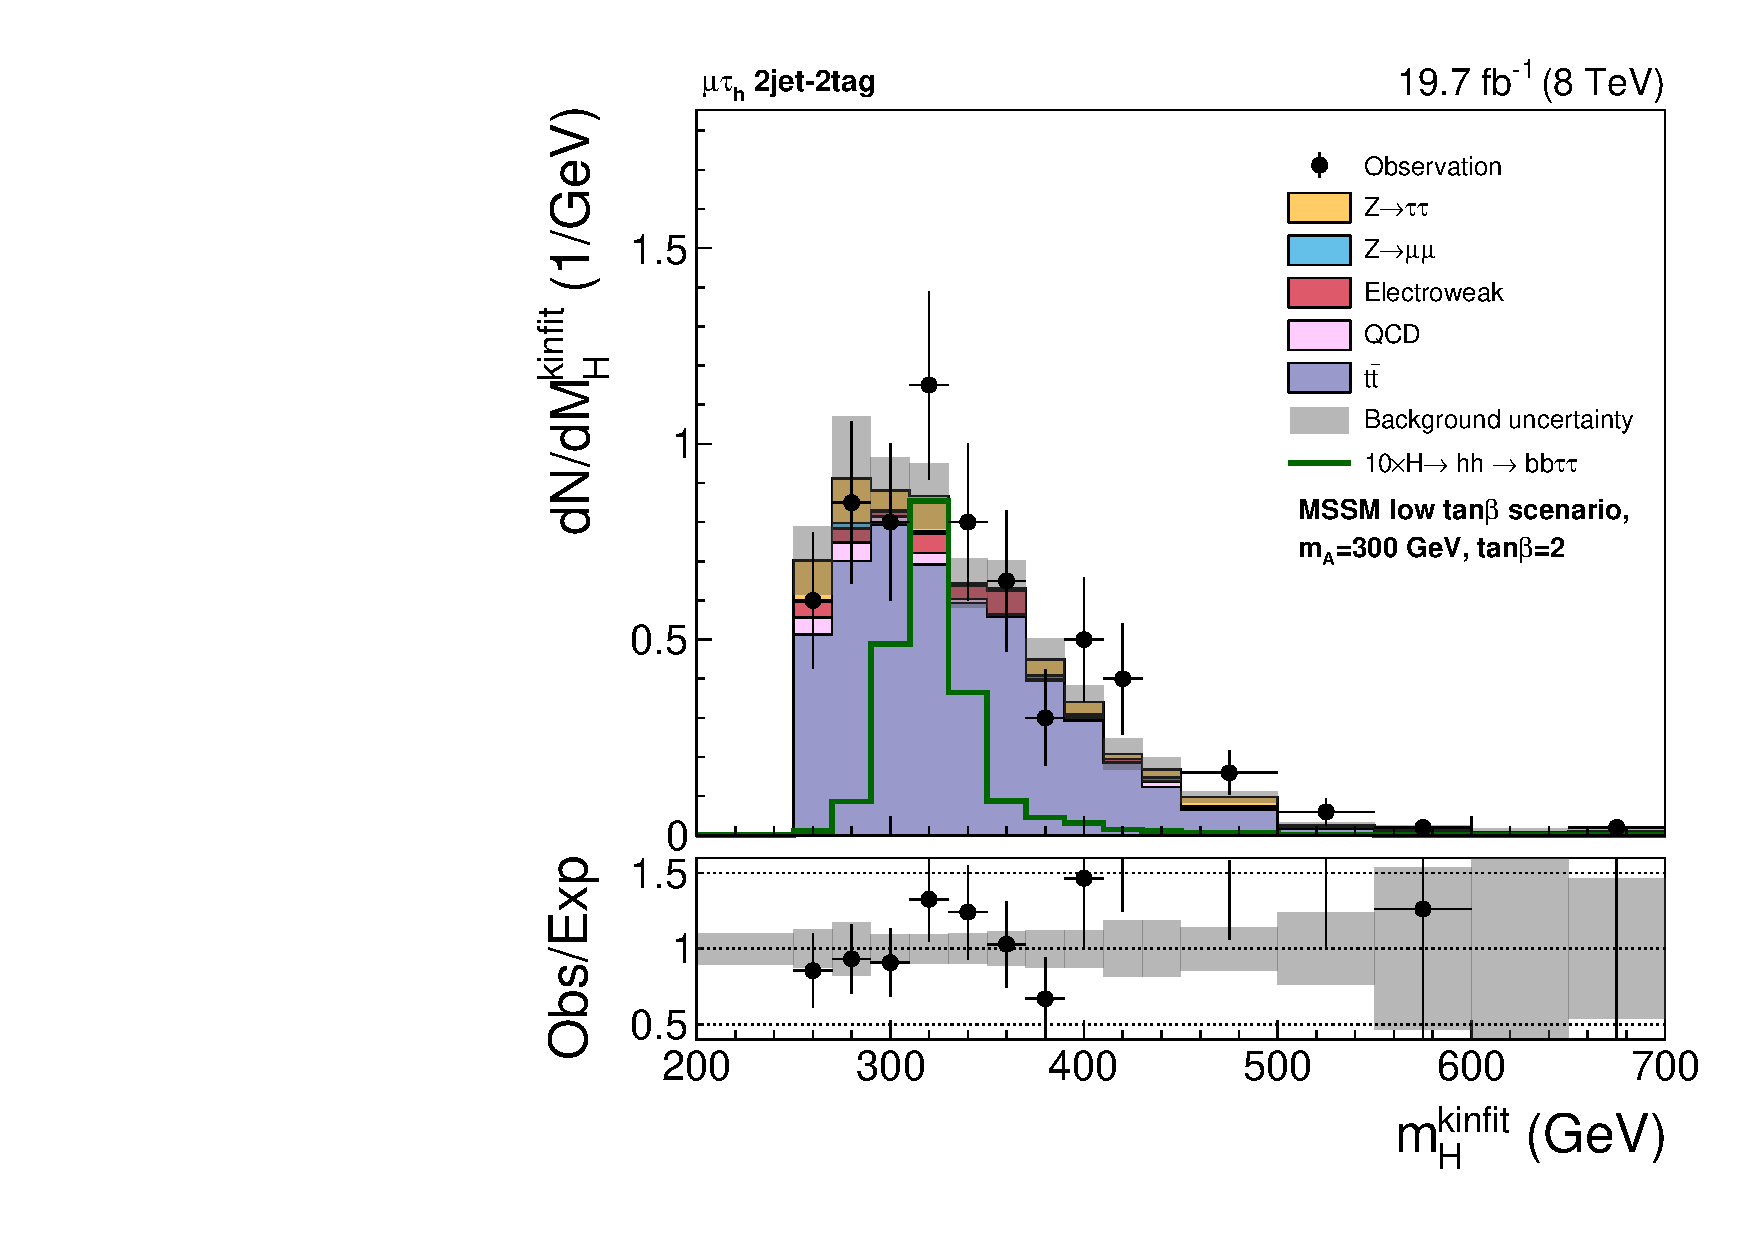
\includegraphics[width=0.5\textwidth]{Hhh/Plots/htt_mt_2_shapes_postfit.pdf}}
\end{center}
\caption[Distributions of $m_{\PHiggs}^{\text{kinfit}}$ in the 2jet-0tag,
2jet-1tag and 2jet-2tag categories of the \mutau channel.]{Distributions of $m_{\PHiggs}^{\text{kinfit}}$ in the (a) 2jet-0tag, (b) 2jet-1tag and (c) 2jet-2tag categories 
of the \mutau channel. The \Htohhtobbtautau signal for \mA~$= 300\,\GeV$ at \tanb~$=2$ in the low-\tanb~MSSM
scenario, multiplied by 10, is also overlaid. Note that at low \tanb~\mA$\neq$\mH, at the point in the MSSM scenario
that is considered \mH~is around 
around $316\,\GeV$.}
\label{fig:hhh_results_mhkinfit_mutau}
\end{figure}

\begin{figure}[h!]
\begin{center}
\subfloat[2jet-0tag]{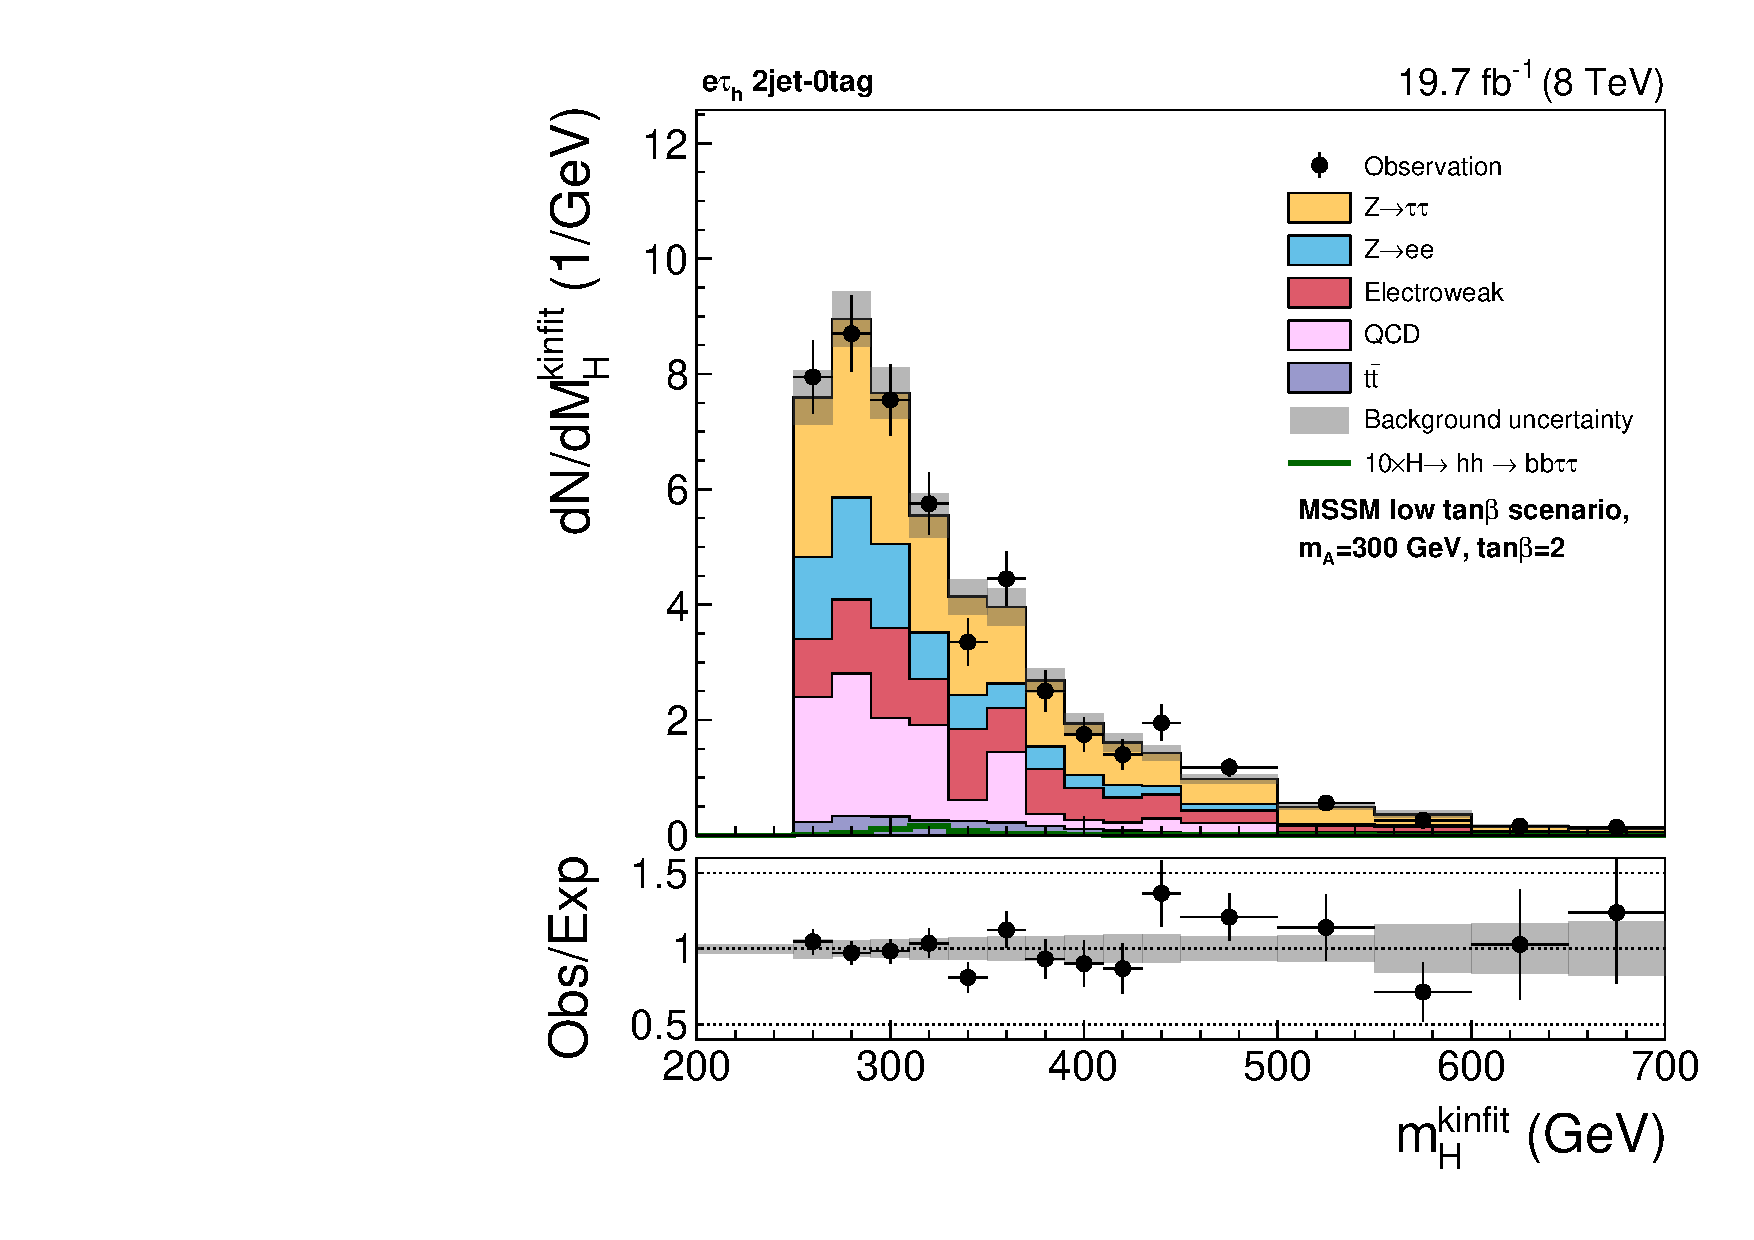
\includegraphics[width=0.5\textwidth]{Hhh/Plots/htt_et_0_shapes_postfit.pdf}}
\subfloat[2jet-1tag]{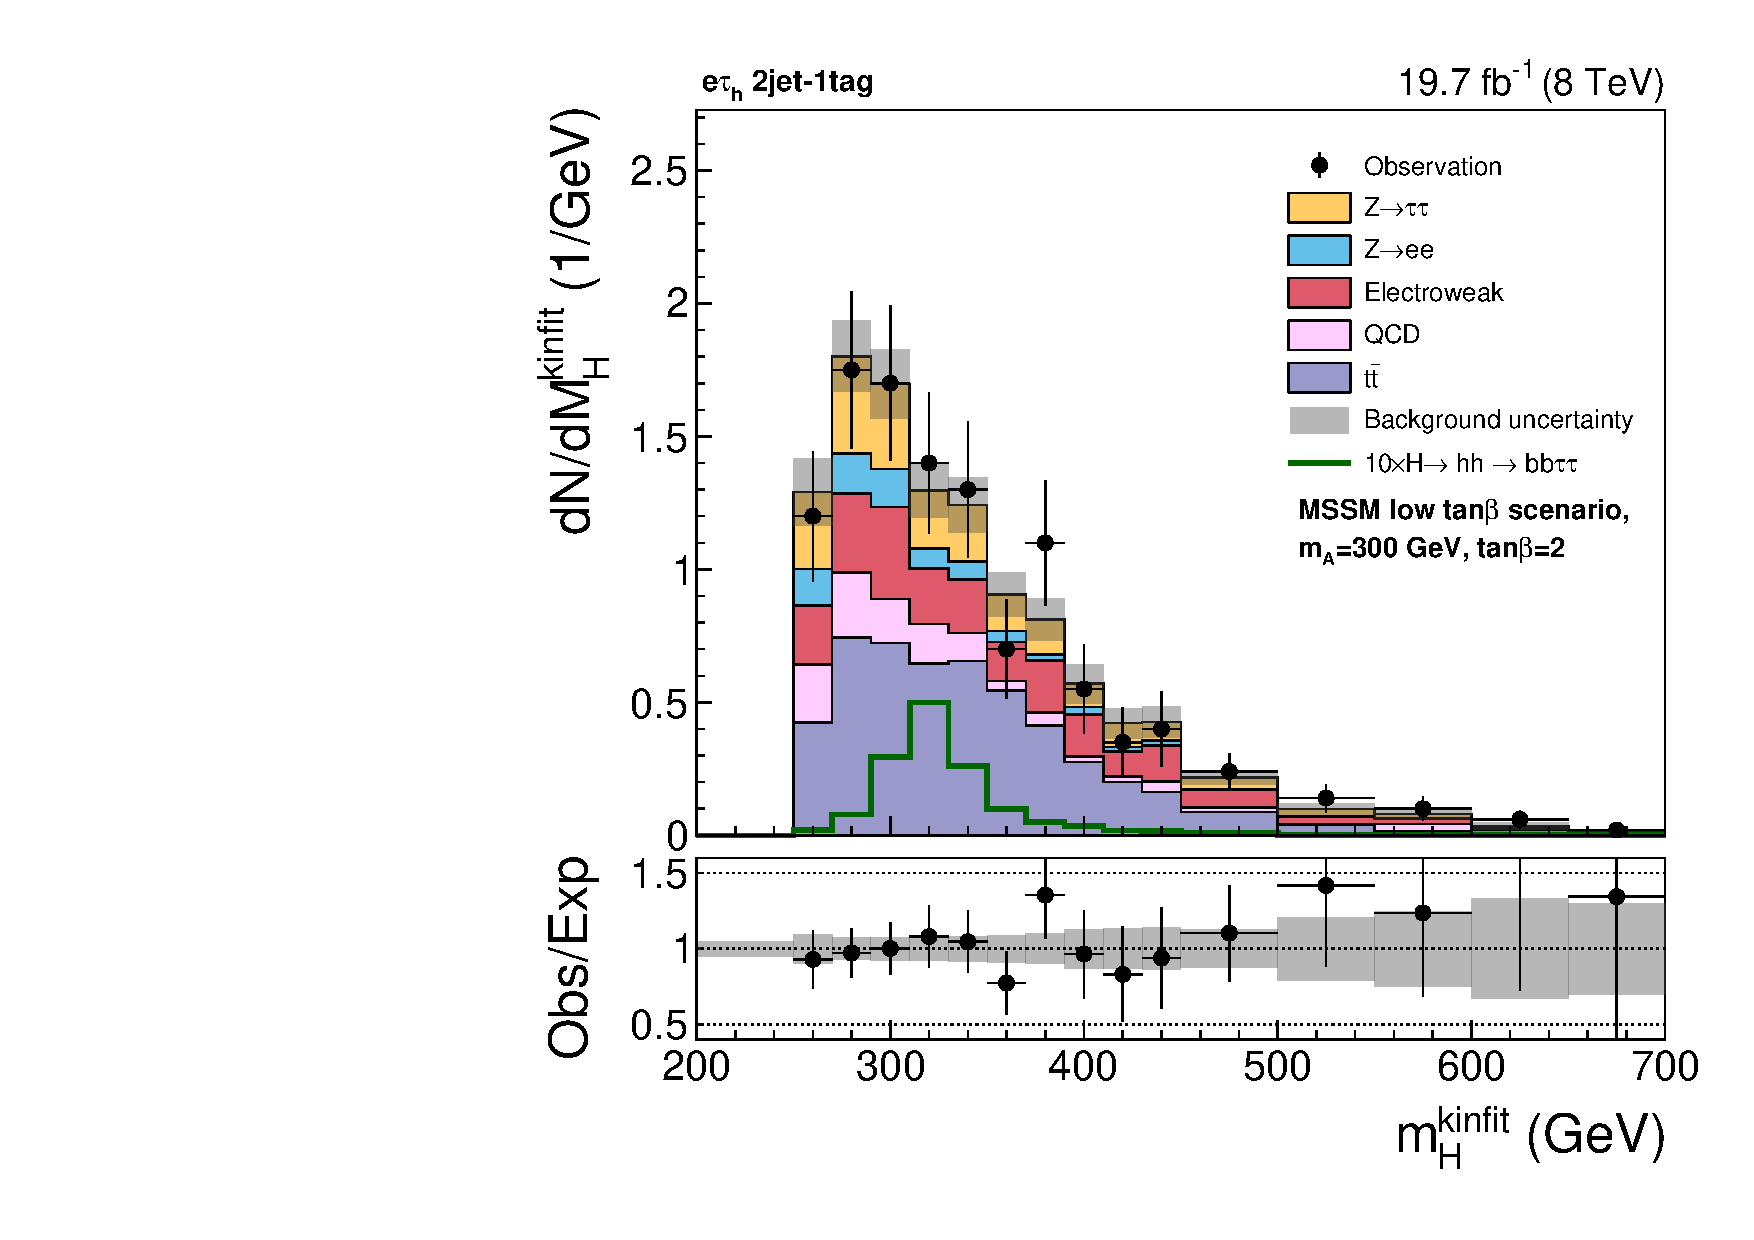
\includegraphics[width=0.5\textwidth]{Hhh/Plots/htt_et_1_shapes_postfit.pdf}}~\\
\subfloat[2jet-2tag]{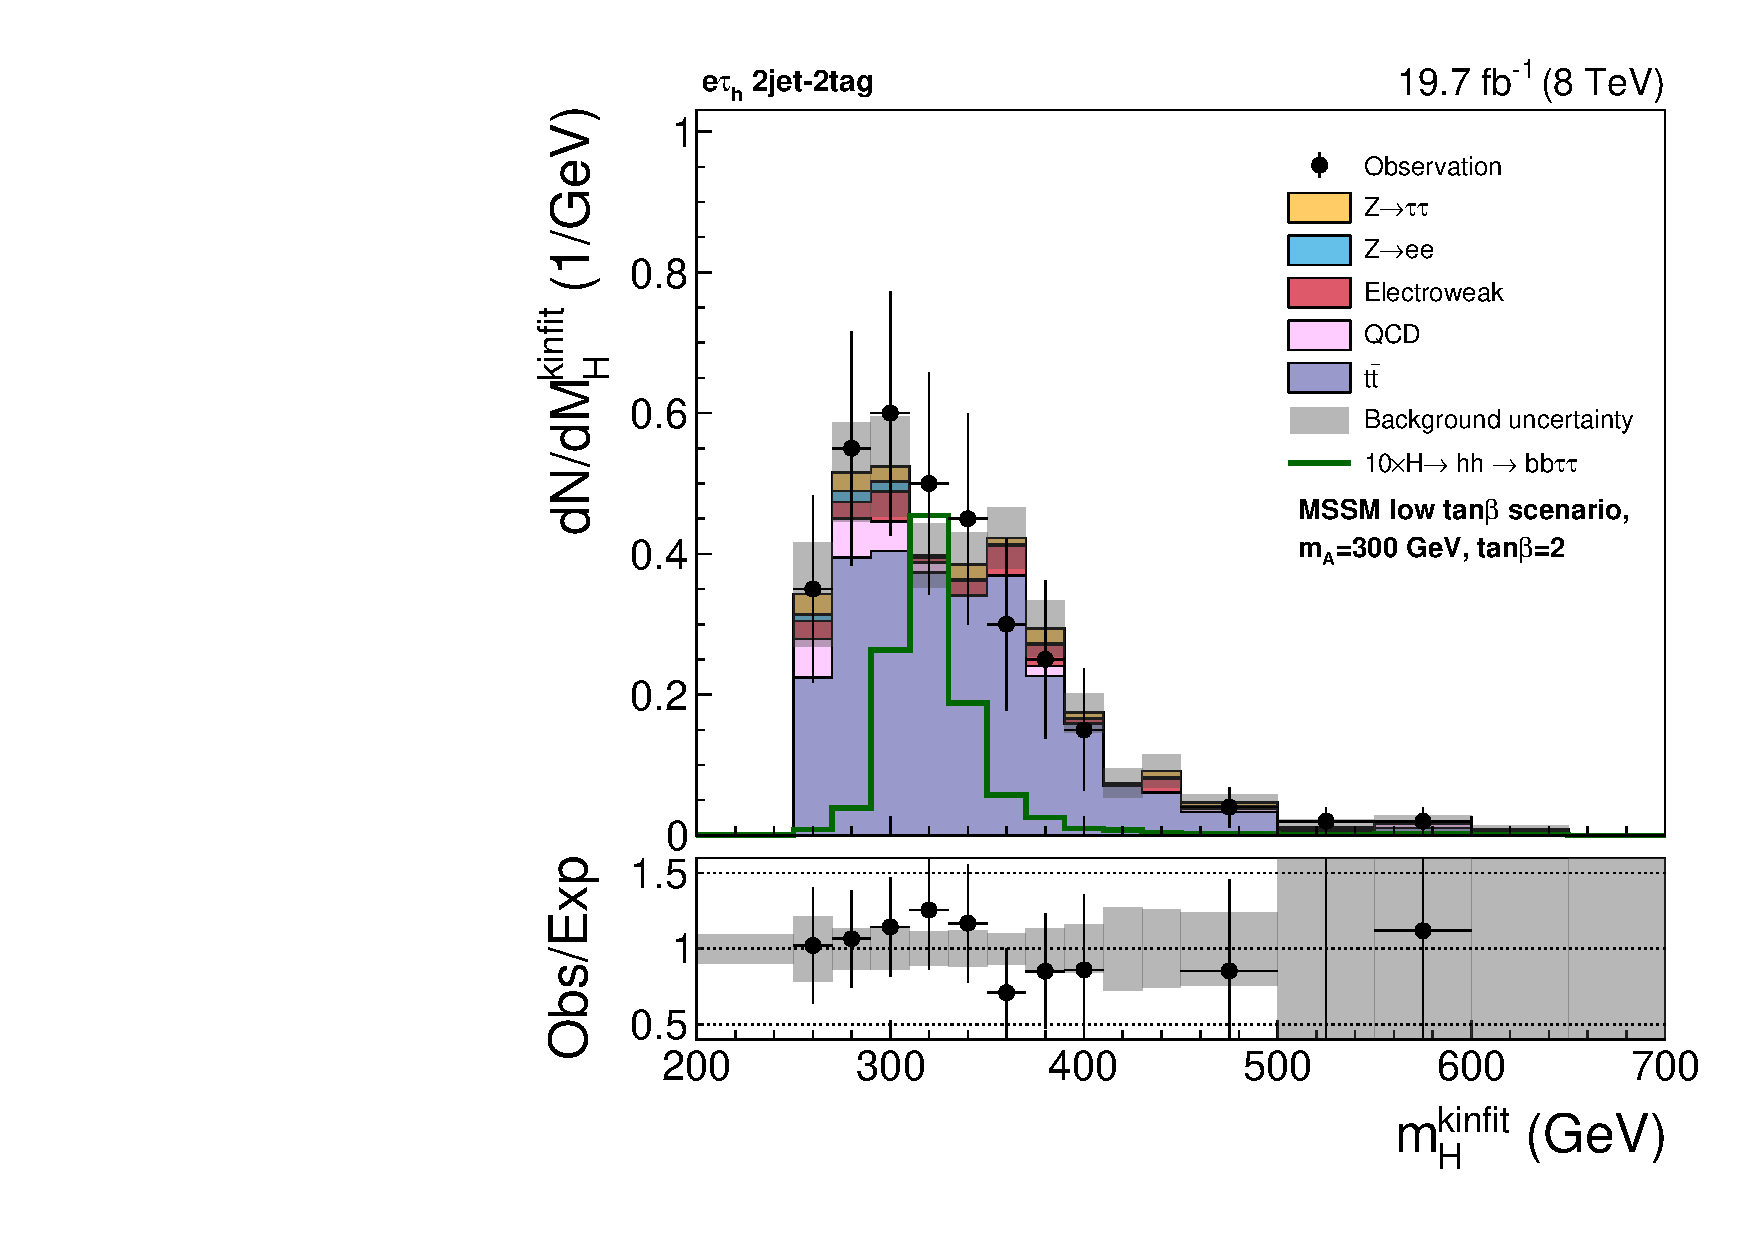
\includegraphics[width=0.5\textwidth]{Hhh/Plots/htt_et_2_shapes_postfit.pdf}}
\end{center}
\caption[Distributions of $m_{\PHiggs}^{\text{kinfit}}$ in the 2jet-0tag,
2jet-1tag and 2jet-2tag categories of the \etau channel.]{Distributions of $m_{\PHiggs}^{\text{kinfit}}$ in the (a) 2jet-0tag, (b) 2jet-1tag and (c) 2jet-2tag categories 
of the \etau channel. The \Htohhtobbtautau signal for \mA~$= 300\,\GeV$ at \tanb~$=2$ in the low-\tanb~MSSM
scenario, multiplied by 10, is also overlaid. Note that at this low value of \tanb~\mA$\neq$ \mH, in 
this case \mH~is around $316\,\GeV$.}
\label{fig:hhh_results_mhkinfit_etau}
\end{figure}

None of these distributions show hints of an excess of observed events above the background expectation. 
The model-independent 95\% \ac{CL} expected and observed upper limits
on \xsbr are shown in 
figure \ref{fig:hhh_results_modelindep}a, with figure \ref{fig:hhh_results_modelindep}b 
showing the expected limit per channel. These figures include the contribution from the 
\tautau channel not described in this chapter. The expected upper limit
on the \Htohhtobbtautau process is around $0.3\,\picobarn$, the observed ranges
from $0.2\,\picobarn$ at low mass to $0.4\,\picobarn$ at high mass. 
The \mutau channel is the most sensitive at masses lower than $320\,\GeV$, with 
the \tautau channel being the most sensitive beyond this mass point. The \etau channel is always
less sensitive than the \mutau channel, but at low mass it is still more sensitive than the \tautau 
channel.

\begin{figure}[h!]
\begin{center}
\subfloat[]{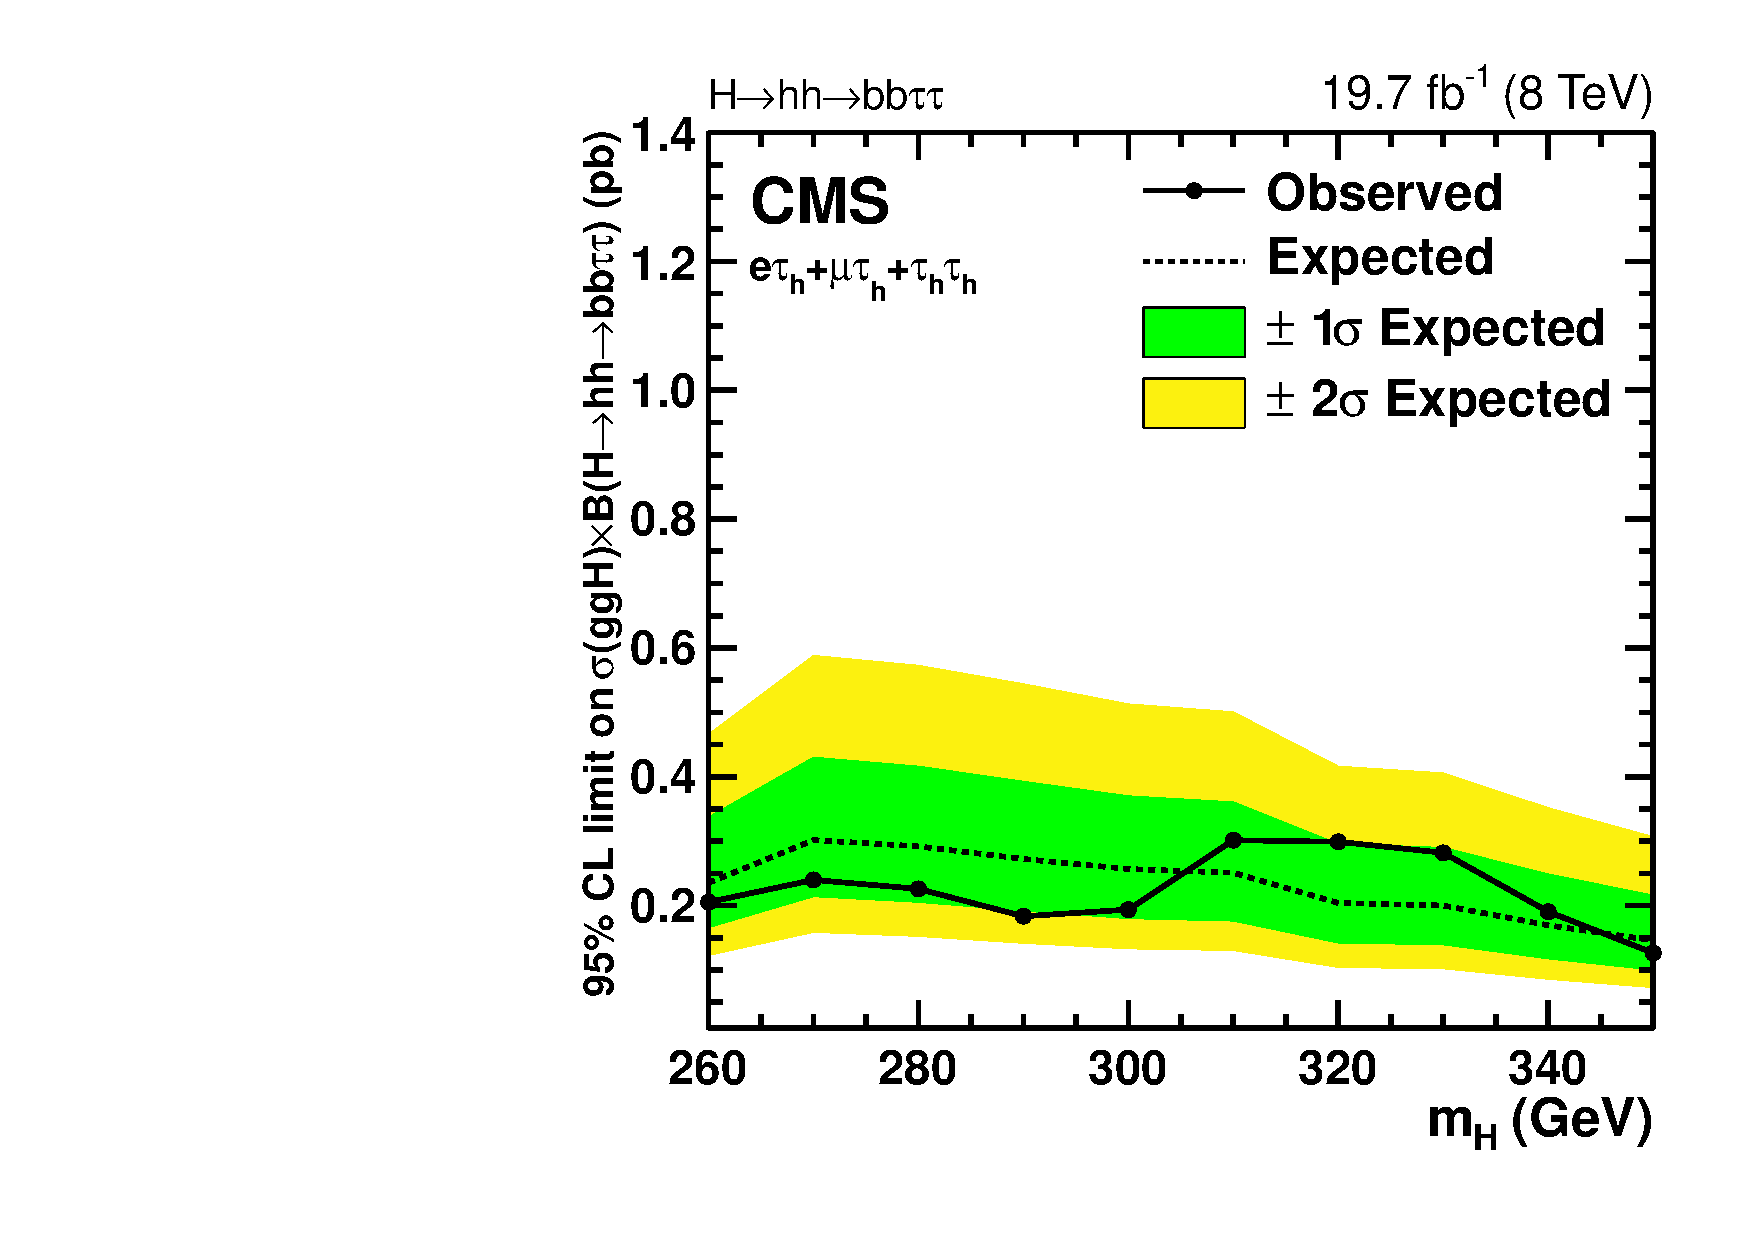
\includegraphics[width=0.5\textwidth]{Hhh/Plots/CMS-HIG-14-034_Figure_008-d.pdf}}
\subfloat[]{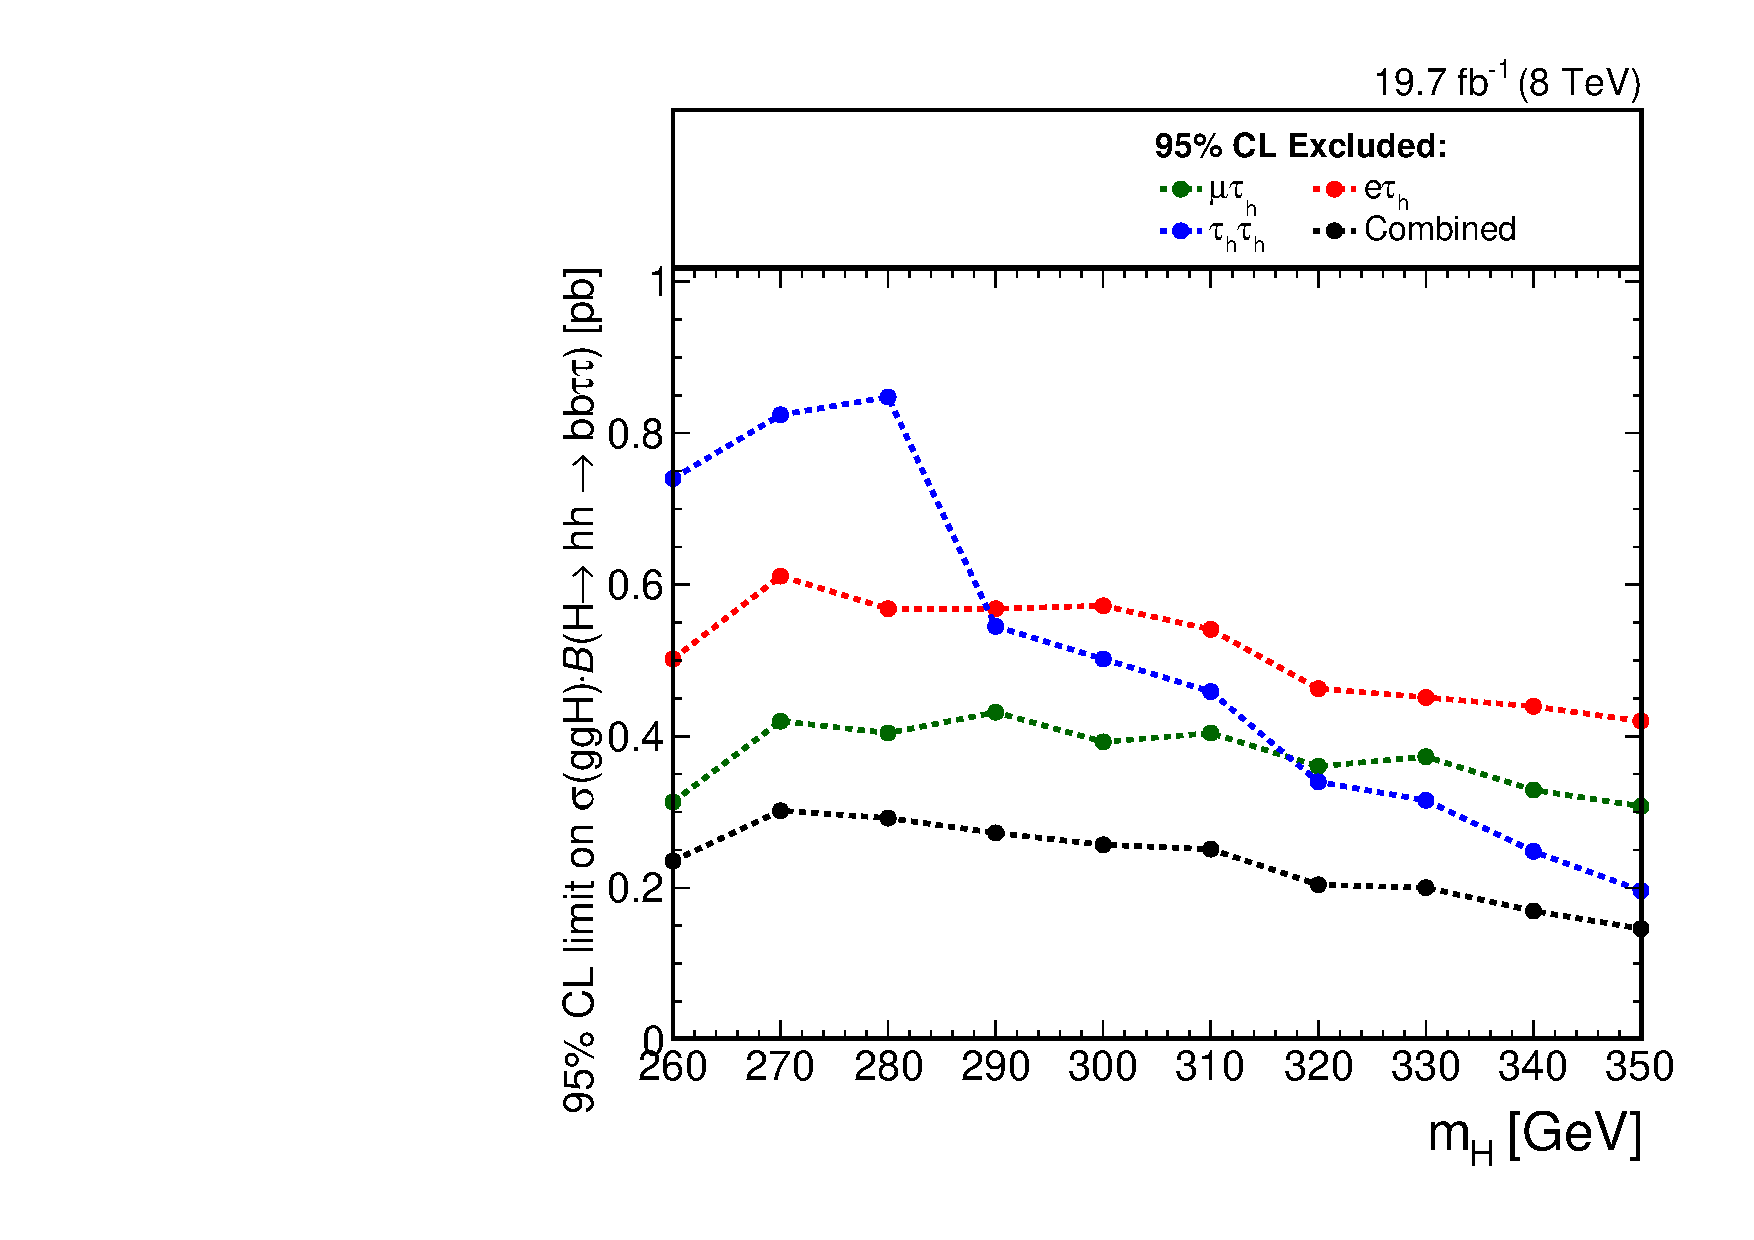
\includegraphics[width=0.5\textwidth]{Hhh/Plots/hhh_limit_comparison.pdf}}
\caption[Expected and observed 95\% CL upper limits on 
\xsbr for the \Htohhtobbtautau process.]{Expected and observed 95\% \ac{CL} upper limits on \xsbr  
for the \Htohhtobbtautau process. In (a) the three final states of \etau, \mutau and \tautau are combined \cite{CMS-HIG-14-034}.
(b) Shows the expected 95\% \ac{CL} upper limits on \xsbr for the \Htohhtobbtautau
process, separated by channel. The blue line shows the limit for the \tautau channel, the green line for the \mutau channel, the red line
for the \etau channel and the black line the limit for all three channels combined. Up to around \mH~$= 320\,\GeV$ the \mutau channel is the most
sensitive, with the \tautau channel being more sensitive at higher masses.}
\label{fig:hhh_results_modelindep}
\end{center}
\end{figure}

%\begin{figure}[h!]
%\begin{center}
%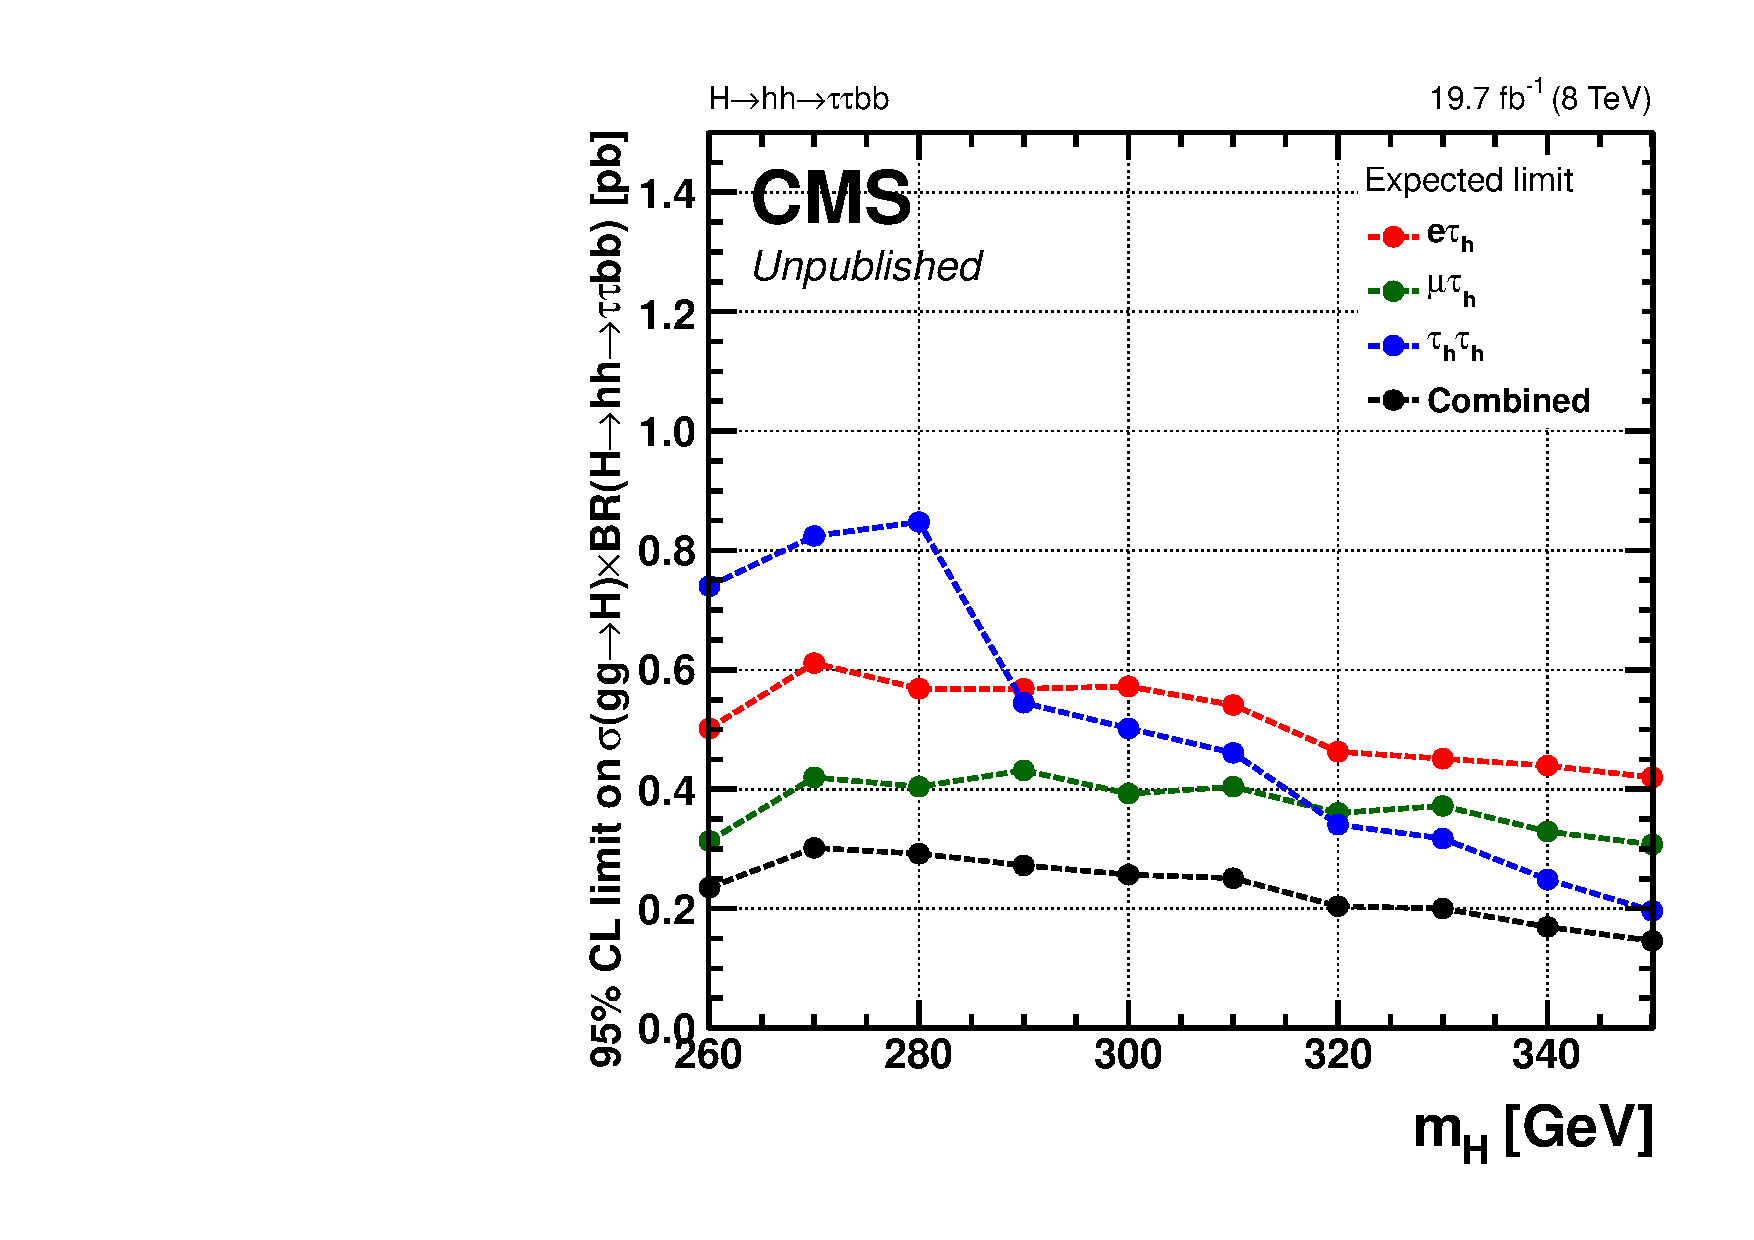
\includegraphics[width=0.7\textwidth]{Hhh/Plots/CMS-HIG-14-034_Figure-aux_033.pdf}
%\caption{Expected 95\% CL upper limits on cross-section times branching ratio for the \Htohhtobbtautau process.
%The blue line represents the limit for the \tautau channel, the green line for the \mutau channel and the
%red line for the \etau channel. The black line shows the limit for all three channels combined. We see that up to around
%$m_H = 320$ GeV the \mutau channel is the most sensitive, with the \tautau channel being more sensitive at higher masses. FIXME remake this plot!}
%\label{fig:hhh_results_modelindep_perchannel}
%\end{center}
%\end{figure}


\subsection{Model-dependent results}
\label{sec:hhh_results_modeldep}
The results of the analysis are interpreted in two scenarios, a type-II \ac{2HDM} and the low-\tanb~MSSM
scenario, both discussed in chapter \ref{chap:theory}.

\subsubsection{Interpretation in a type-II 2HDM}
\label{sec:hhh_results_modeldep_2HDM}
As discussed in section \ref{sec:theory_2HDM}, a \ac{2HDM} has more
free parameters than a particular \ac{MSSM} benchmark scenario. To leave
just two free parameters, it is enough to fix the masses of the five Higgs bosons
and take the quartic couplings to be zero.
For the interpretation shown here the assumption that \mA=\mH=\mHplus~$=300\,\GeV$ is made.

The couplings of the Higgs bosons to quarks and leptons, and of the heavy Higgs bosons to other
particles, are defined by $\alpha$ and $\beta$, as in table \ref{tab:hhh_2HDM_couplings}.

\begin{table}[htp]
\begin{center}
\caption{Couplings in the type-II 2HDM}
\begin{tabular}{@{}ll@{}}
\toprule
\textbf{Decay} & \textbf{Coupling}\\
\midrule
$\PHiggslight \rightarrow$ up-type quarks & $\text{SM coupling} \times \frac{\cos{\alpha}}{\sin{\beta}}$ \\
$\PHiggslight \rightarrow$ down-type quarks, leptons & $\text{SM coupling} \times -\frac{\sin{\alpha}}{\cos{\beta}}$ \\
$\PHiggs \rightarrow \PHiggslight\PHiggslight$ & $\sim$ \cosba $\times$ terms containing masses,\\
 & mixing angles, quartic couplings \\
$\PHiggsps \rightarrow \PZ\PHiggslight$ & $\sim$ \cosba\\
\bottomrule
\end{tabular}
\label{tab:hhh_2HDM_couplings}
\end{center}
\end{table}

The interpretations are made in the \cosba-\tanb~plane. Figure \ref{fig:HhhandAZh2HDMOverlaid}
shows the observed and expected exclusion at 95\% \ac{CL} for the \Htohh
and \AtoZh analyses, overlaid on the \xsbr.
The exclusion contours have some interesting features, most of which can be explained by the couplings
in table \ref{tab:hhh_2HDM_couplings}. When \cosba=0, in the alignment limit, the couplings
of all particles are exactly \ac{SM}-like. This is reflected in the \Htohh and \AtoZh branching ratios, 
which both vanish as \cosba~approaches zero. This leads to the corridor of non-exclusion down the 
centre of the graphs in figure \ref{fig:HhhandAZh2HDMOverlaid}. Additionally,
as the coupling of the \PHiggslight to pairs of b-quarks or tau leptons is proportional 
to $\frac{\sin{\alpha}}{\cos{\beta}}$, the branching ratios of \Htohhtobbtautau
and \AtoZhtolltautau vanish when $\alpha = 0$, leading to the corridor of non-exclusion
at \cosba $ > 0$ and low \tanb~in the \AtoZh figure. A similar corridor is starting
to become visible in the \xsbr structure of the \Htohh interpretation, but
the analysis is not yet sensitive enough to actually observe it.
%Additional regions of non--exclusion at low \tanb and \cosba near -1 are visible in the \Htohh 
%interpretation, these are a result of the complex \Htohh branching ratio.

\begin{figure}[h!]
\begin{center}
\subfloat[\Htohhtobbtautau]{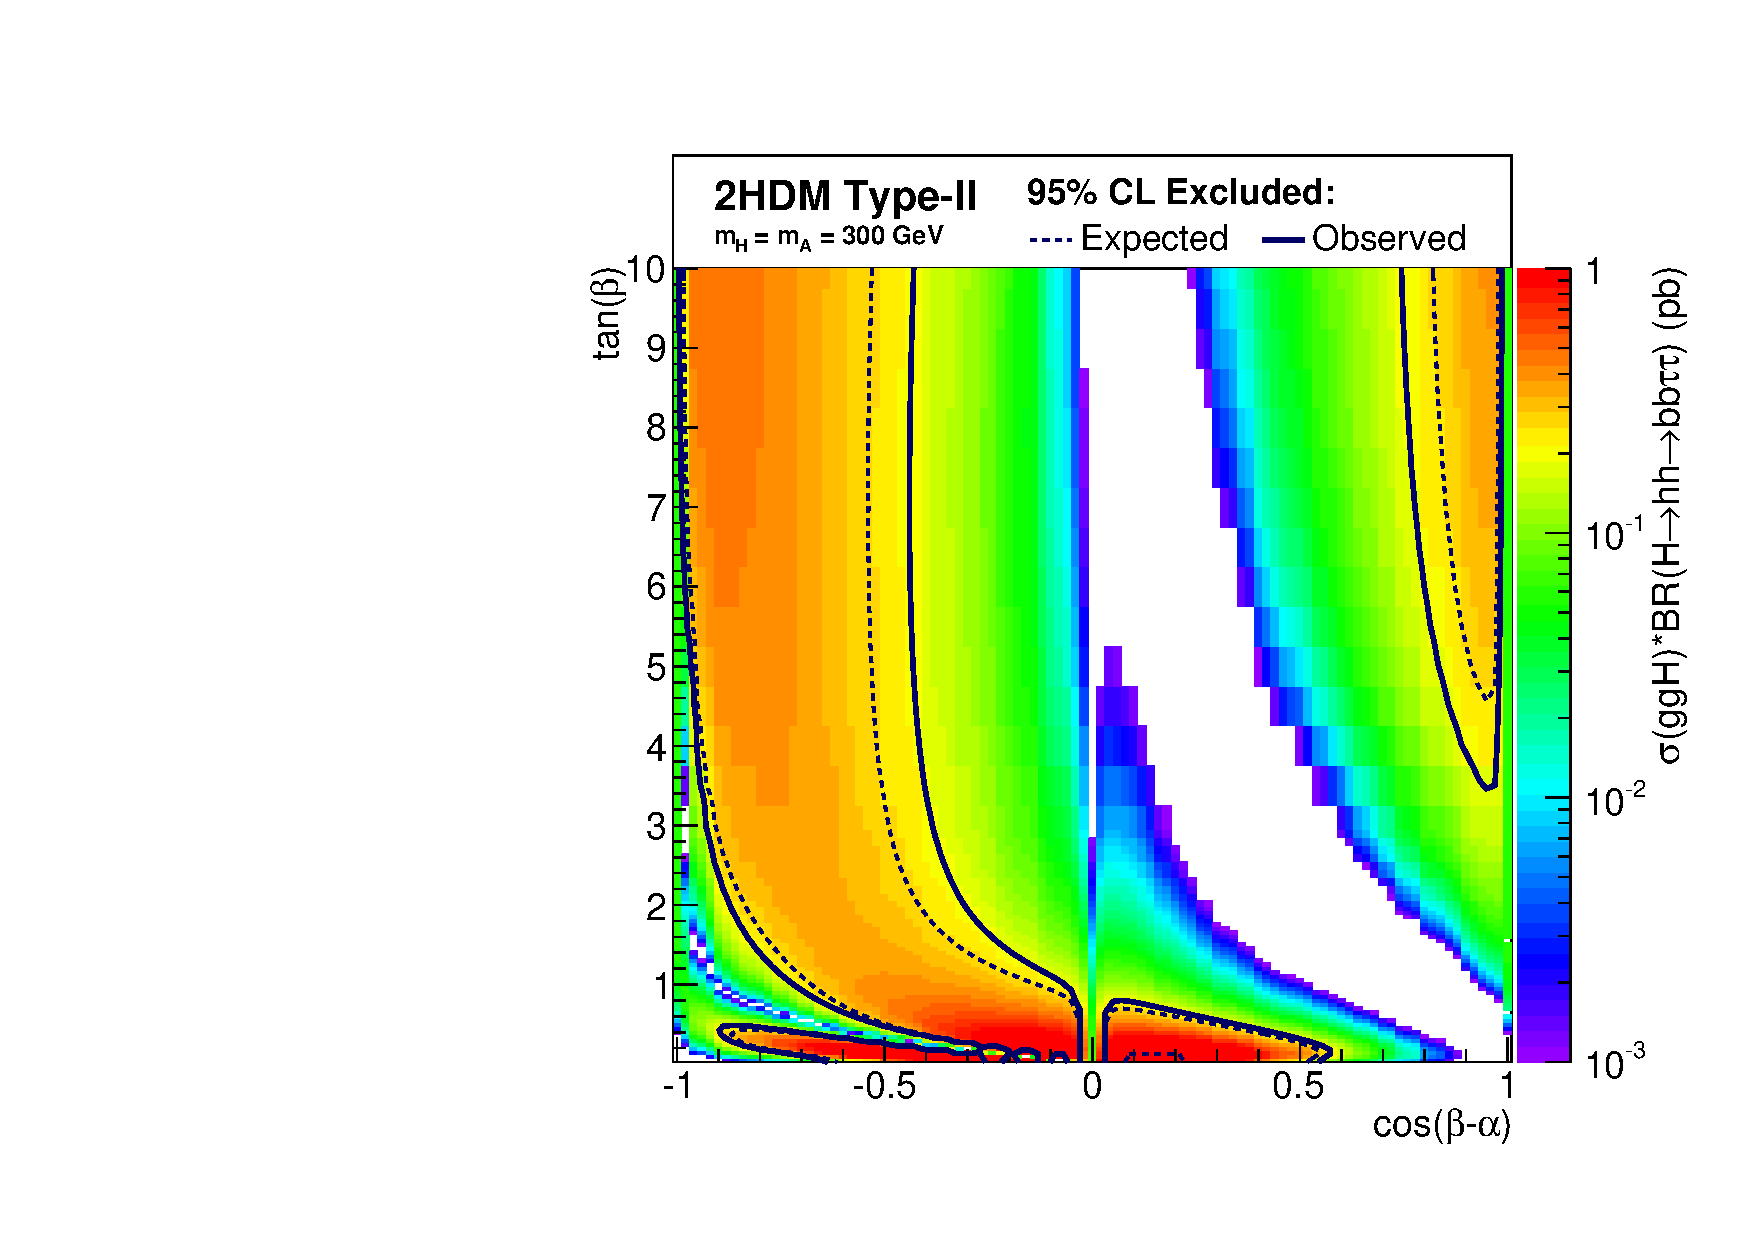
\includegraphics[width=0.5\textwidth]{Hhh/Plots/Hhh2HDM.pdf}}
\subfloat[\AtoZhtolltautau]{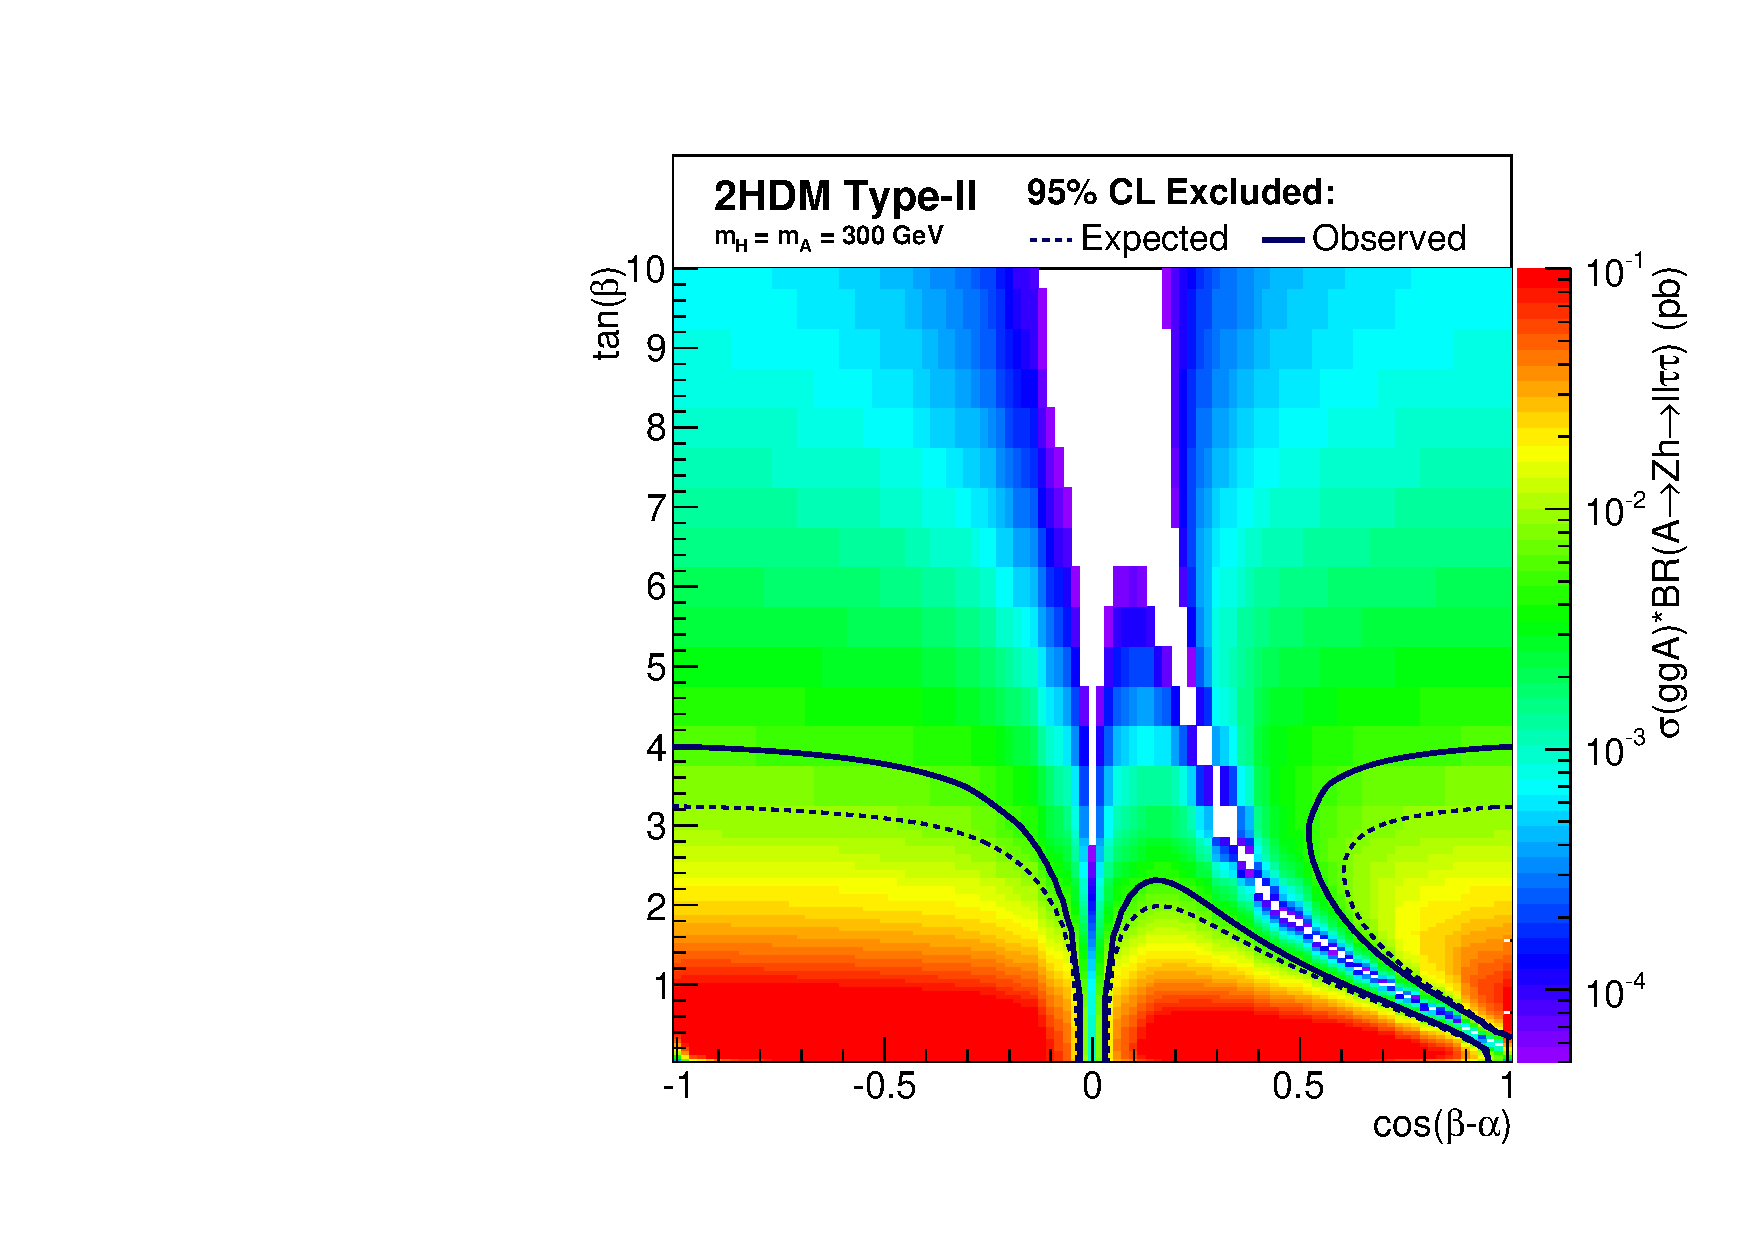
\includegraphics[width=0.5\textwidth]{Hhh/Plots/AZh2HDM.pdf}}
\caption[Search for \Htohhtobbtautau and search for \AtoZhtolltautau
interpreted in a type-II 2HDM, assuming \mA=\mH=\mHplus~$=300\,\GeV$.]{Search for (a) \Htohhtobbtautau and (b) \AtoZhtolltautau interpreted in a type-II 
\ac{2HDM}, assuming \mA=\mH=\mHplus~$= 300\,\GeV$. The expected (dashed line)
and observed (solid line) exclusion contours at 95\% \ac{CL} are overlaid
on the \xsbr of the searched-for process.
Regions of the \cosba-\tanb~plane where the 
\xsbr is larger than the model-independent upper limit set for $m_{\PHiggs} = 300\,\GeV$ 
(see figures \ref{fig:AZhUpperLimits} and \ref{fig:hhh_results_modelindep}) are excluded.}
\label{fig:HhhandAZh2HDMOverlaid}
\end{center}
\end{figure}

%\begin{figure}[h!]
%\begin{center}
%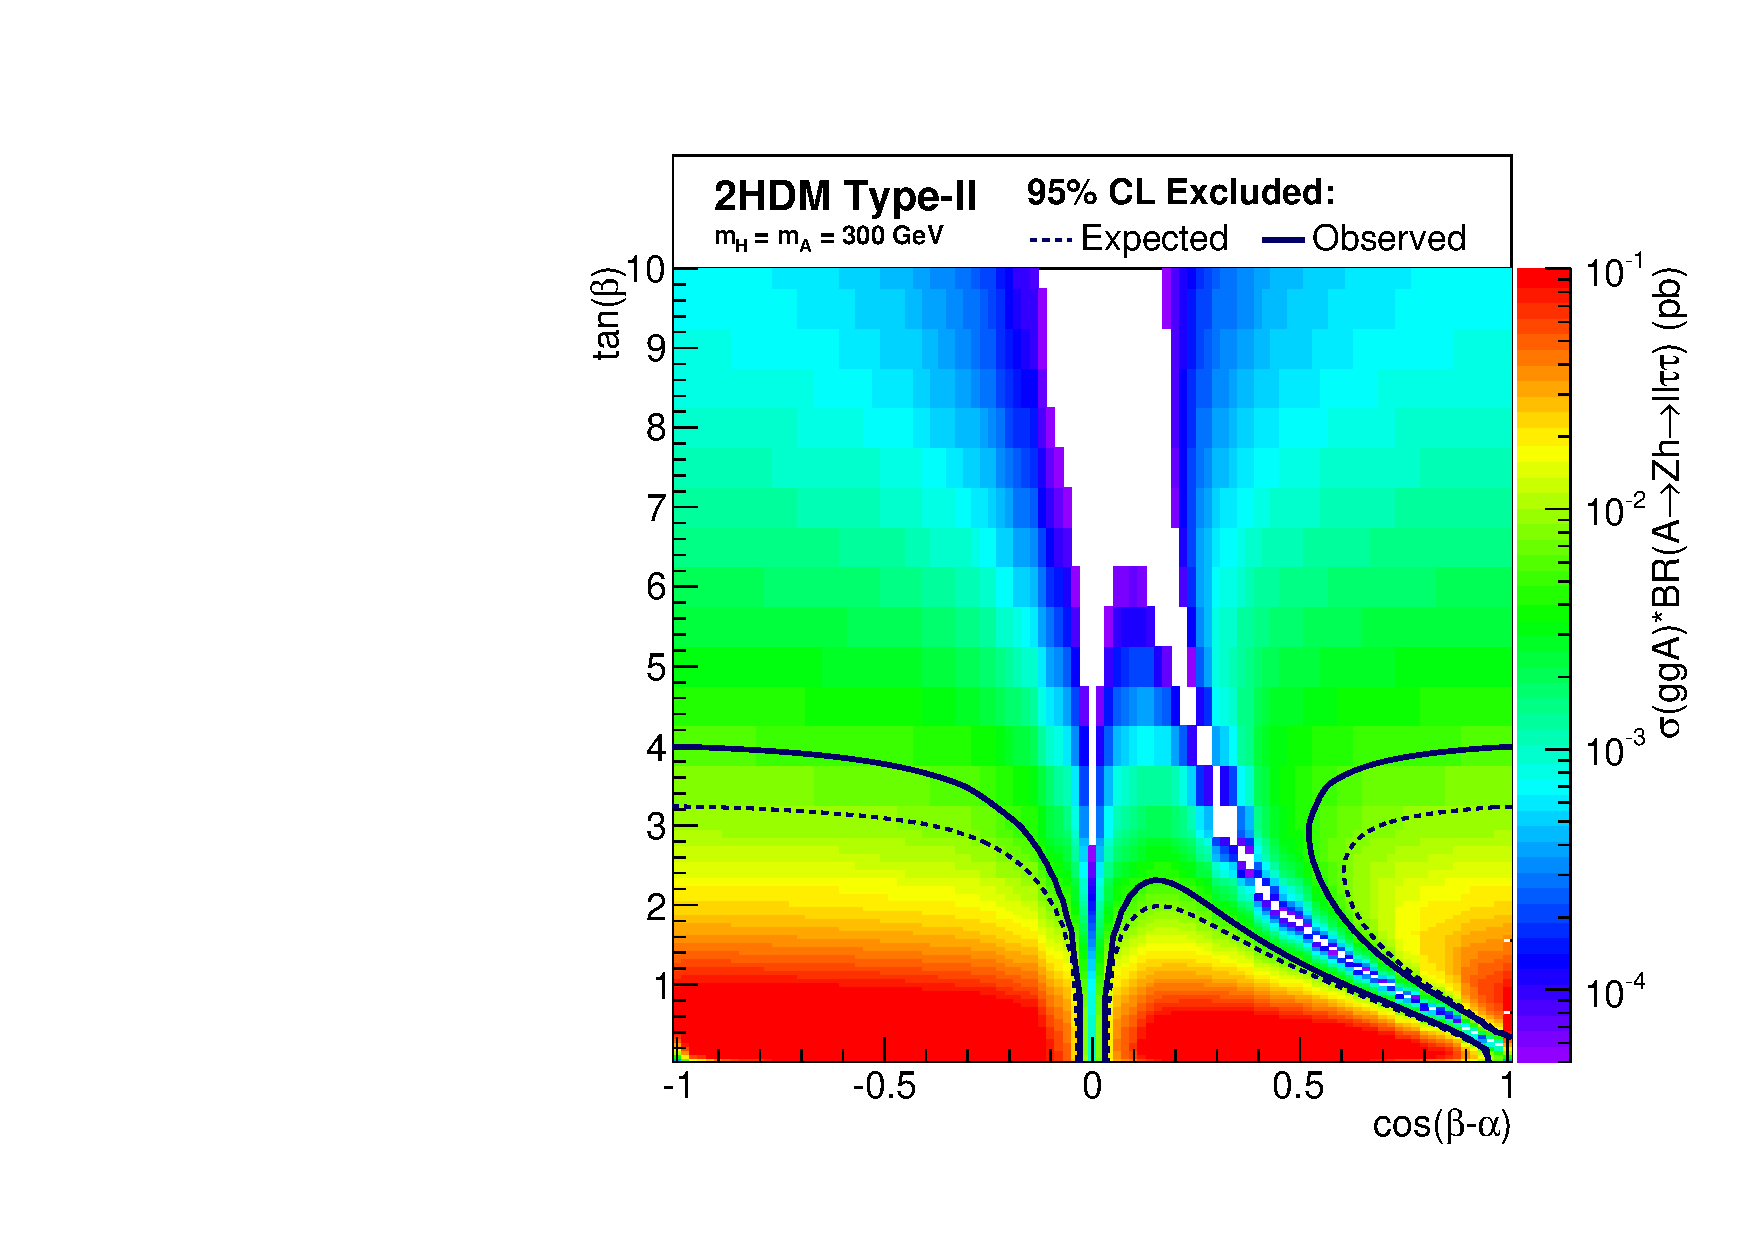
\includegraphics[width=0.85\textwidth]{Hhh/Plots/AZh2HDM.pdf}
%\caption{Search for \AtoZhtolltautau interpreted in a type II 
%2HDM, assuming $m_{H} = m_{A} = m_{H^{+}} = 300$ GeV. The expected (dashed line)
%and observed (solid line) exclusion contours at 95\% confidence level are overlaid
%on the cross--section of $gg\rightarrow \PHiggsps$ production
%times the branching ratio of \PHiggsps into \Zhtolltautau.
%Regions of the \cosba-\tanb plane where the cross--section times branching
%ratio is larger than the model-independent upper limit set for $m_{A} = 300 $~GeV 
%(see figure \ref{fig:AZhUpperLimits}) are excluded.}
%\label{fig:AZh2HDMOverlaid}
%\end{center}
%\end{figure}

A combined interpretation of both analyses in this model is presented
in figure \ref{fig:HhhAZhMSSM2HDM}a. Some of the features discussed earlier
in this section are also visible in this combined interpretation.


\subsubsection{Interpretation in the low-\tanb~MSSM scenario}
\label{sec:hhh_results_modeldep_lowtb}
The low-\tanb~MSSM scenario, as discussed in section \ref{sec:mssm_theory_lowtb},
is an \ac{MSSM} scenario that has been adapted to allow \mh~$=125 \pm 3\,\GeV$ for \tanb~values
as low as 1.  

Figure \ref{fig:HhhAndAZhlowtanb}a shows the \xsbr 
of the \Htohhtobbtautau process in the low-\tanb~MSSM scenario. Comparing these values 
to the expected and observed upper limits in figure \ref{fig:hhh_results_modelindep} we 
can see that the \xsbr in this model is, with the exception of a few very small 
areas, lower than the upper limits set by this analysis. This analysis on its own is,
therefore, not sensitive enough to exclude any of the \mA-\tanb~region in this model. Note that
at low \tanb, \mA$\neq$ \mH, and therefore \mH~is not in the studied range of $260$--$350\,\GeV$
everywhere in the \mA-\tanb~plane shown here.

The \AtoZhtolltautau analysis on the other hand can exclude parts of the \mA-\tanb~region
in this model. The expected and observed 95\% \ac{CL} exclusion contours are overlaid 
on the \xsbr for this process in the low-\tanb~MSSM scenario in  
figure \ref{fig:HhhAndAZhlowtanb}b. The sharp drop in \xsbr, and therefore exclusion,
near \mA~$ = 350\,\GeV$ arises from the fact that near this mass the decay $\PHiggsps \rightarrow \Ptop\APtop$ becomes
kinematically allowed, resulting in a reduction of the \AtoZh branching ratio.


\begin{figure}[h!]
\begin{center}
\subfloat[\Htohhtobbtautau]{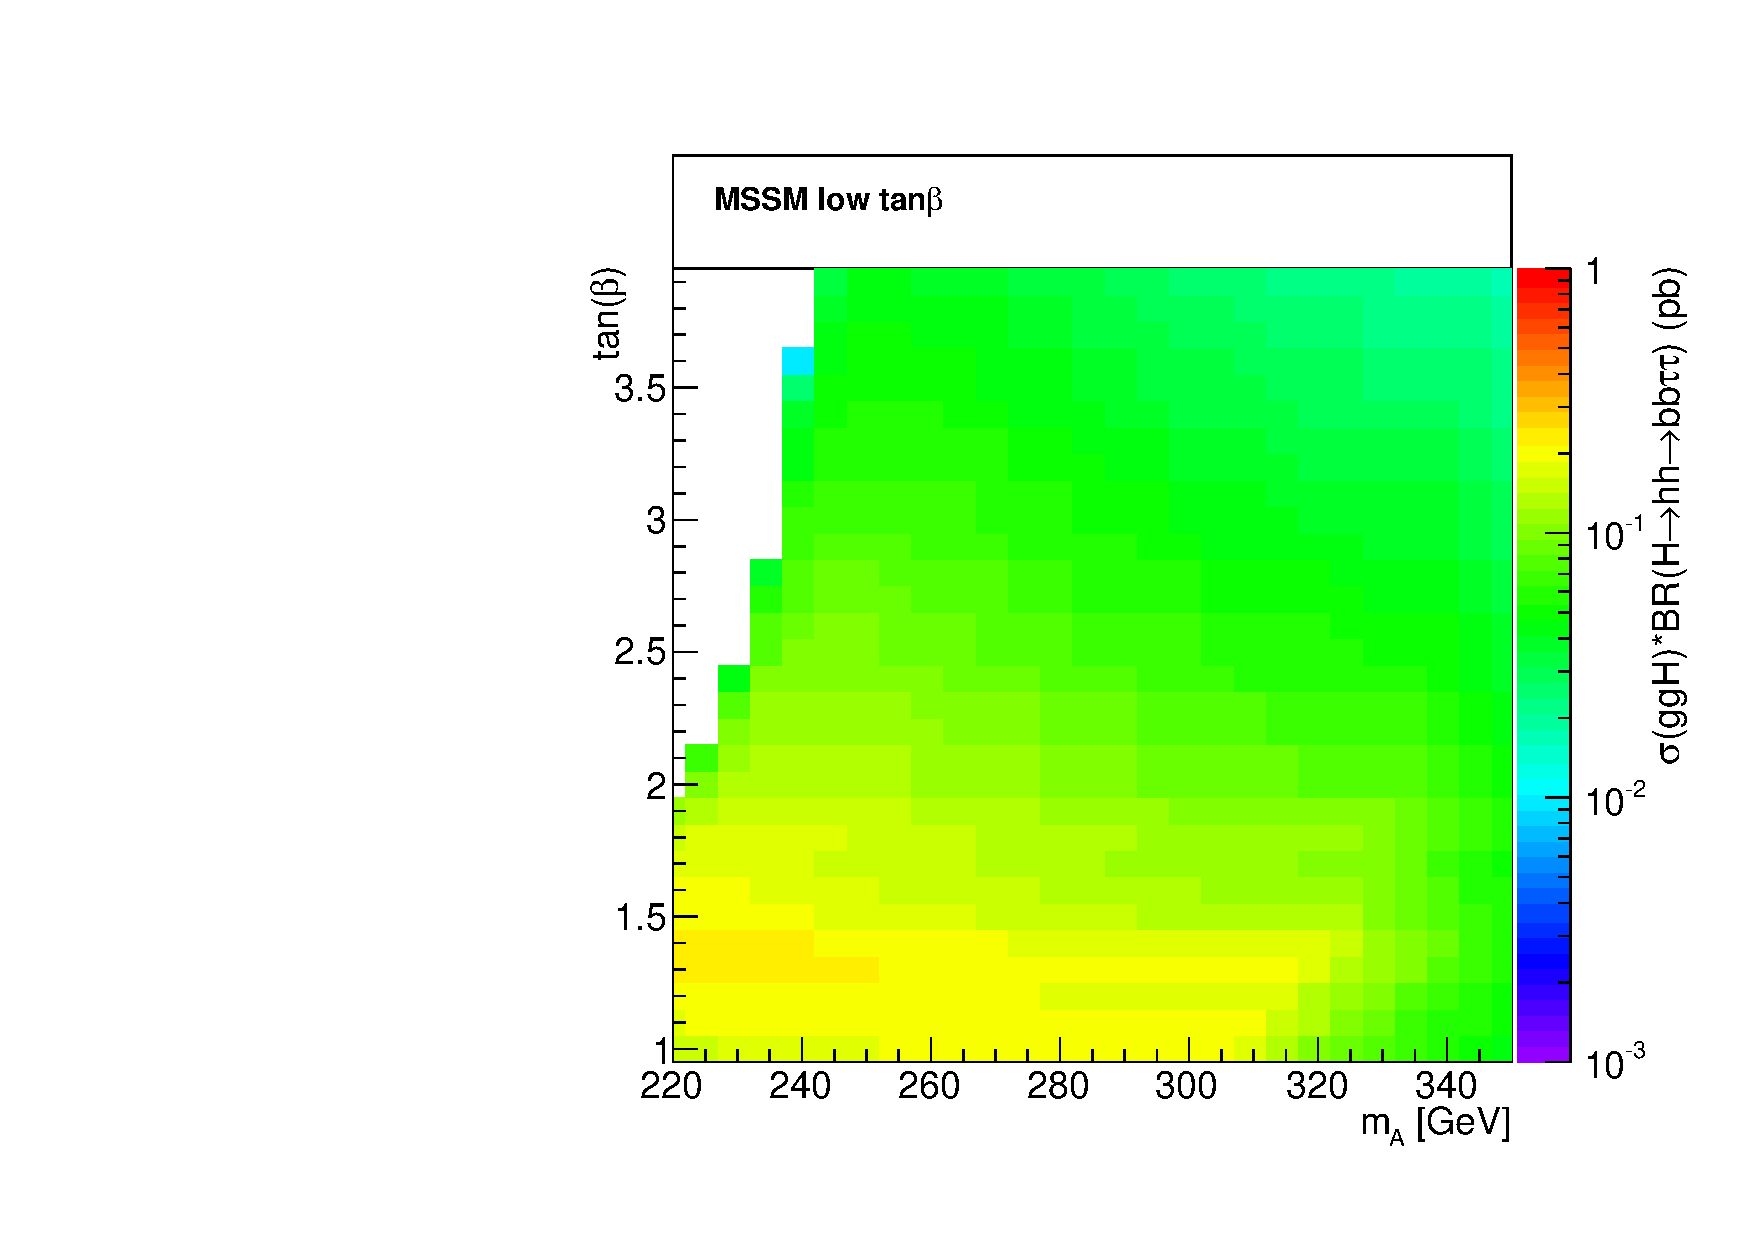
\includegraphics[width=0.5\textwidth]{Hhh/Plots/Hhhlowtbhigh.pdf}}
\subfloat[\AtoZhtolltautau]{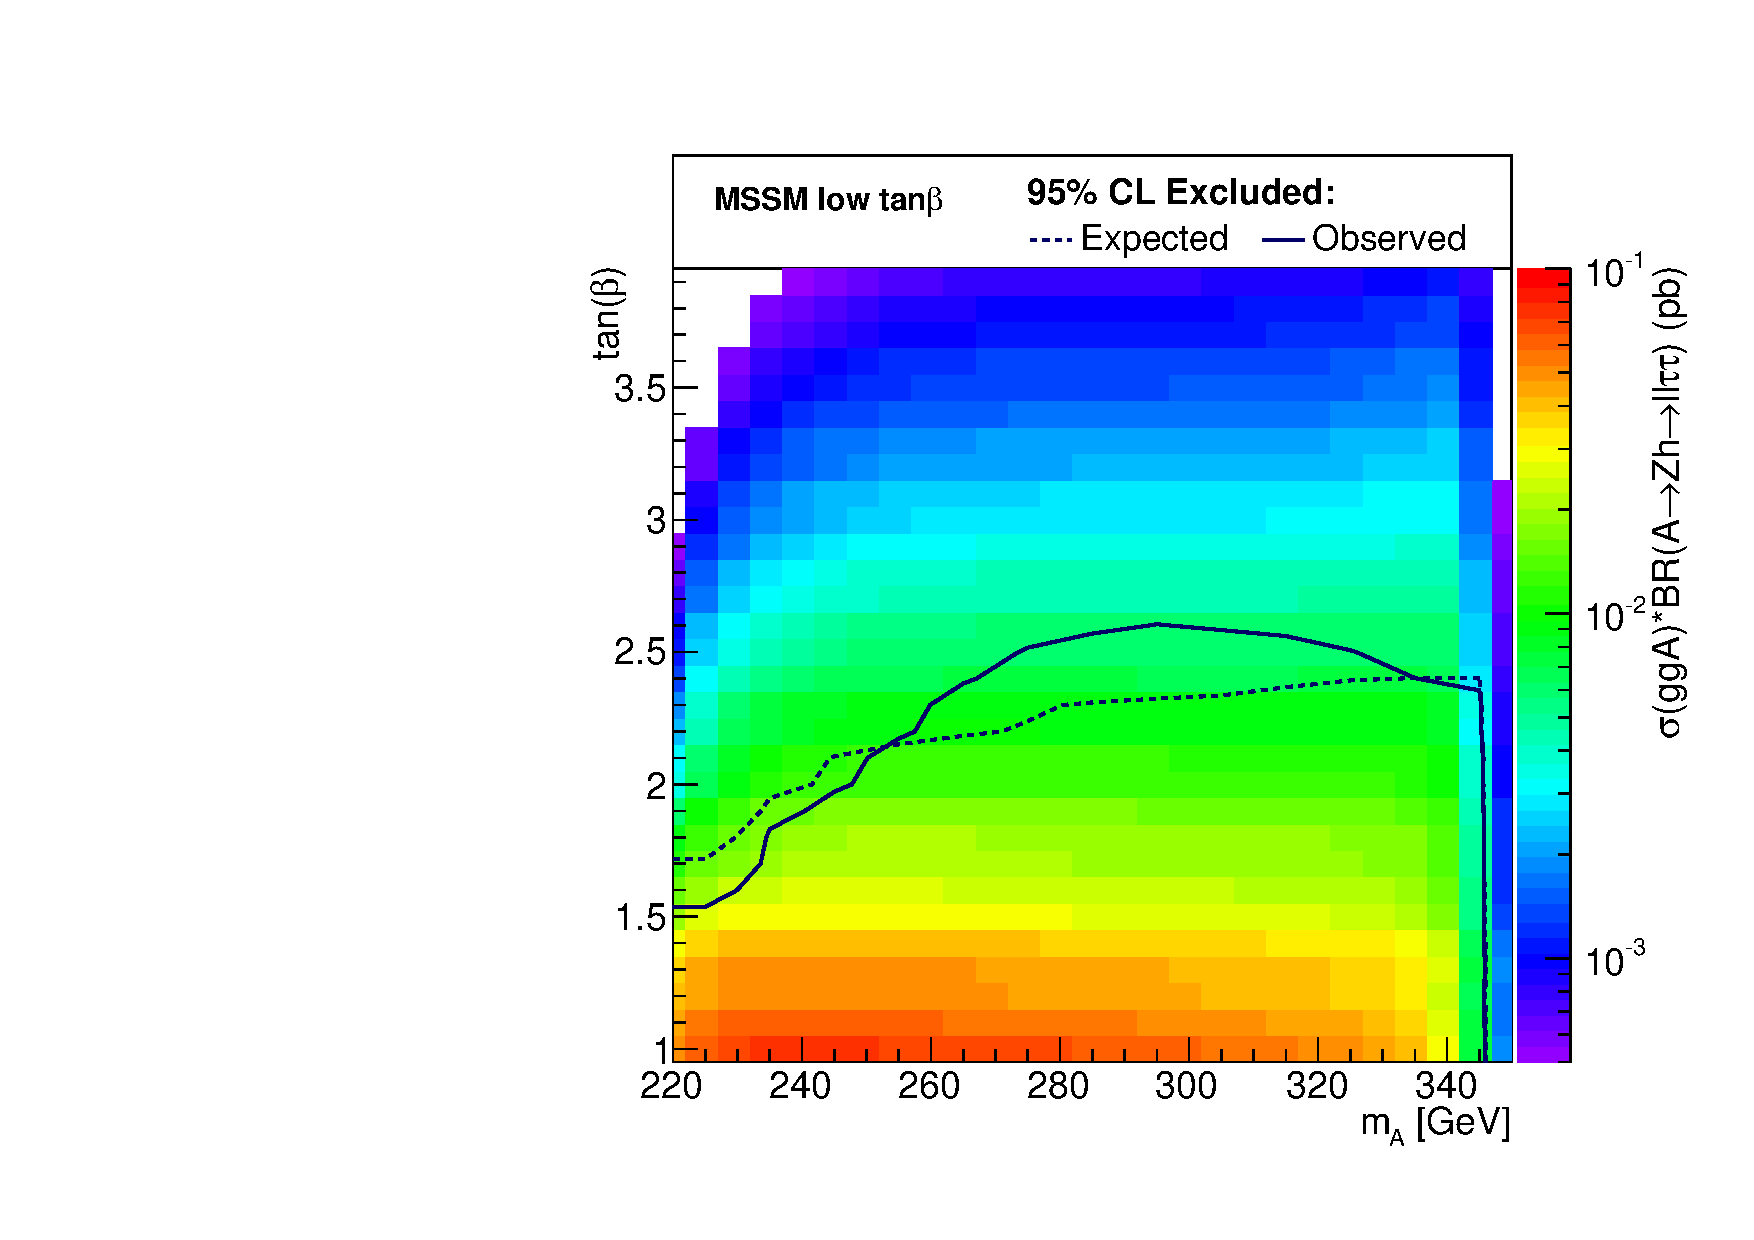
\includegraphics[width=0.5\textwidth]{Hhh/Plots/AZhlowtbhigh.pdf}}
\caption[\xsbr of the \Htohhtobbtautau
process and the \AtoZhtolltautau process in the low-\tanb ~MSSM scenario. The
expected and observed 95\% CL exclusion limits for the \AtoZhtolltautau analysis
in the low \tanb~MSSM scenario have been overlaid.]{The \xsbr of (a) the \Htohhtobbtautau process and (b) the
\AtoZhtolltautau process in the low-\tanb~MSSM scenario. In (b) 
the expected and observed 95\% \ac{CL} exclusion limits for the \AtoZhtolltautau analysis in the low-\tanb~MSSM scenario
have been overlaid on the \xsbr. Areas where the 
\xsbr is larger than the upper limits in figure \ref{fig:AZhUpperLimits} are excluded. The exclusion rapidly drops
off at \mA~$ = 350\,\GeV$ due to the turn-on of the $\PHiggsps \rightarrow$ \ttbar process.
No expected and observed exclusion contours
have been overlaid on (a) as the 
\xsbr is smaller than the upper limits set in figure \ref{fig:hhh_results_modelindep}.}
\label{fig:HhhAndAZhlowtanb}
\end{center}
\end{figure}



%\begin{figure}[h!]
%\begin{center}
%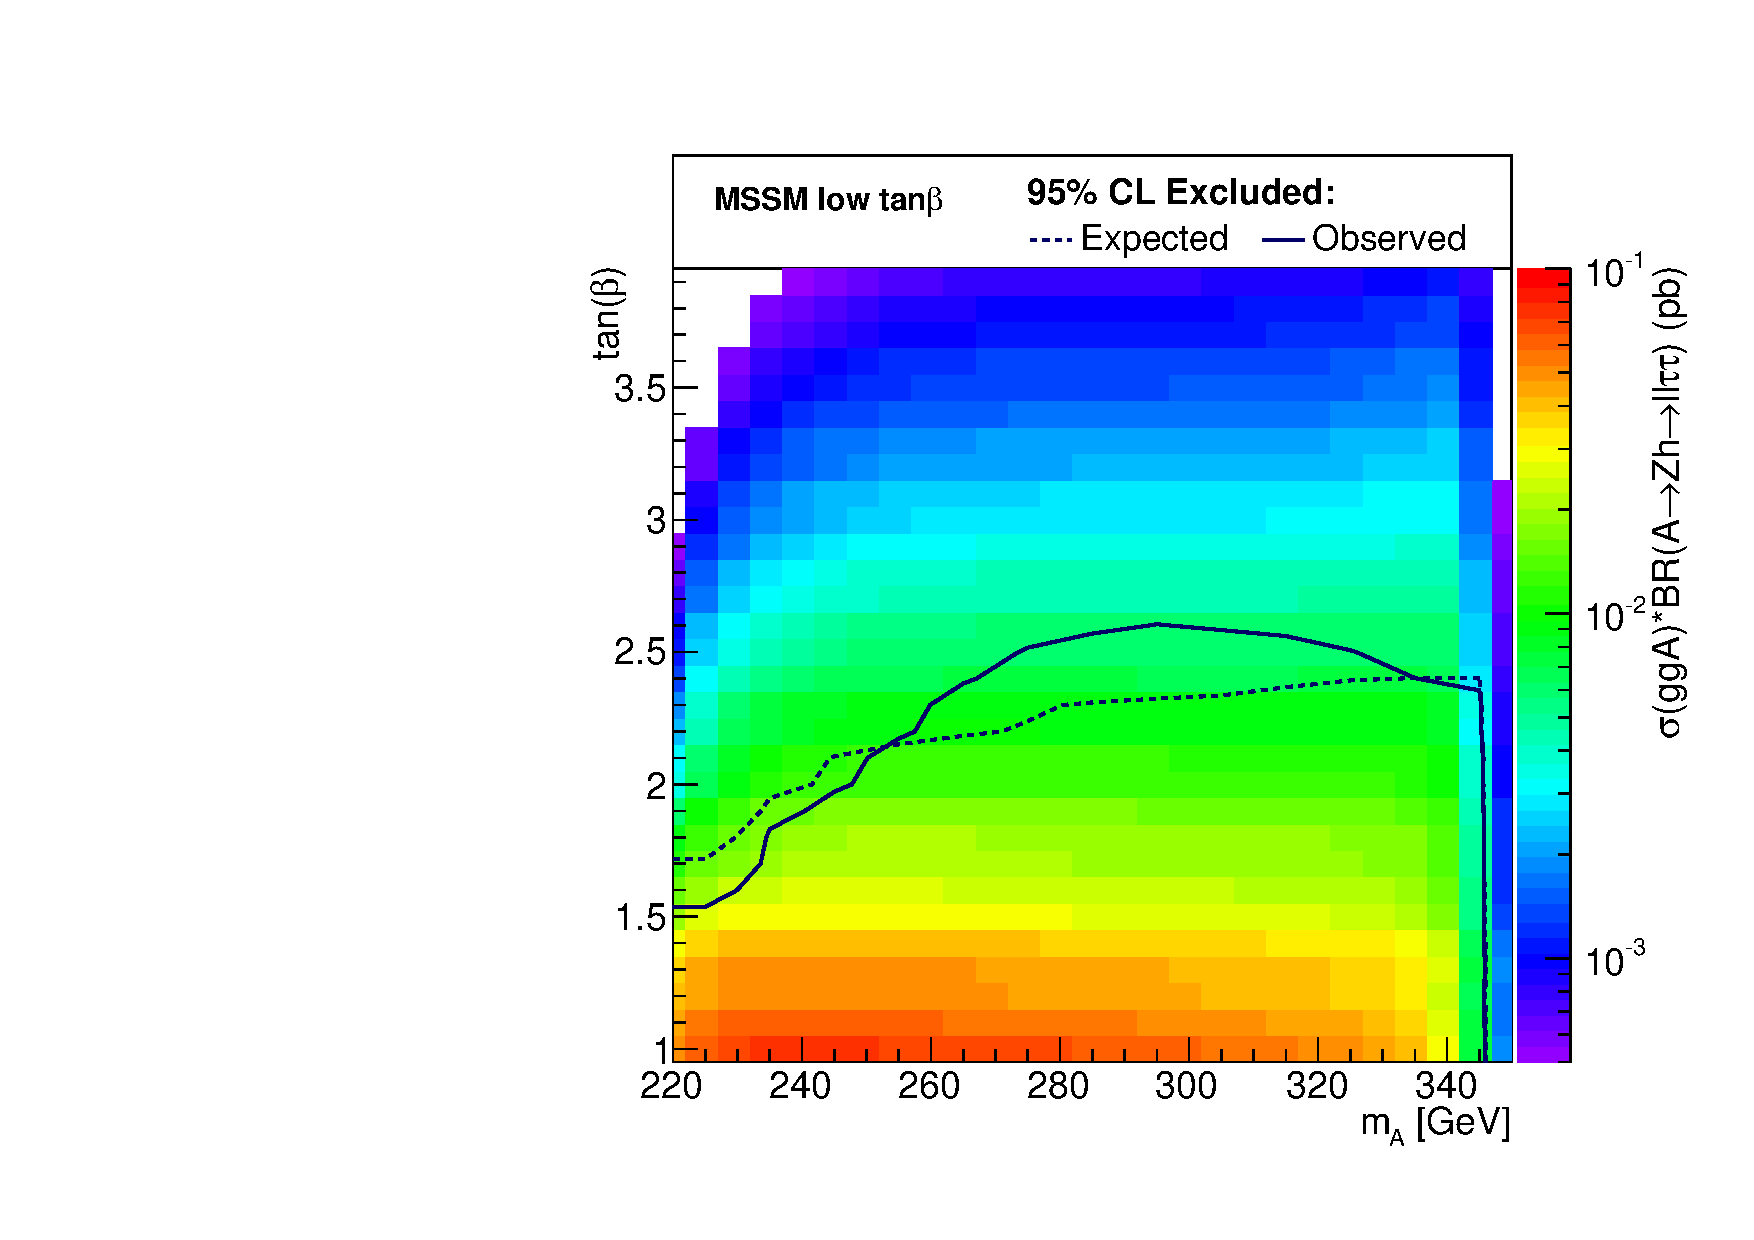
\includegraphics[width=0.85\textwidth]{Hhh/Plots/AZhlowtbhigh.pdf}
%\caption{Expected and observed 95 \% CL exclusion limits for the \AtoZhtolltautau analysis
%in the low \tanb MSSM scenario, overlaid on the cross-section times branching ratio. Areas where
%the cross-section times branching ratio is larger than the upper limits in figure \ref{fig:AZhUpperLimits}
%are excluded. The exclusion rapidly drops off at $m_A = 350$ GeV due to the turn-on of the
%$ \PHiggsps \rightarrow$ \ttbar process.}
%\label{fig:AZhlowtanbOverlaid}
%\end{center}
%\end{figure}


The combined interpretation of both analyses in this model is presented figure 
\ref{fig:HhhAZhMSSM2HDM}b.
%The exclusion in this scenario is driven by the \AtoZh search as the \Htohh search is not
%very sensitive in this model. 
By combining the two analyses a slightly larger amount
of the \mA-\tanb~plane can be excluded than using the \AtoZhtolltautau analysis alone. The features
described for the figure \ref{fig:HhhAndAZhlowtanb}b are also visible in this figure. In a small region of phase
space, at low \mA~and low~\tanb, this scenario predicts a light Higgs boson mass that is not compatible with $125\pm3\,\GeV$.
This region is therefore excluded, as indicated by the red band. 

%\begin{figure}[h!]
%\begin{center}
%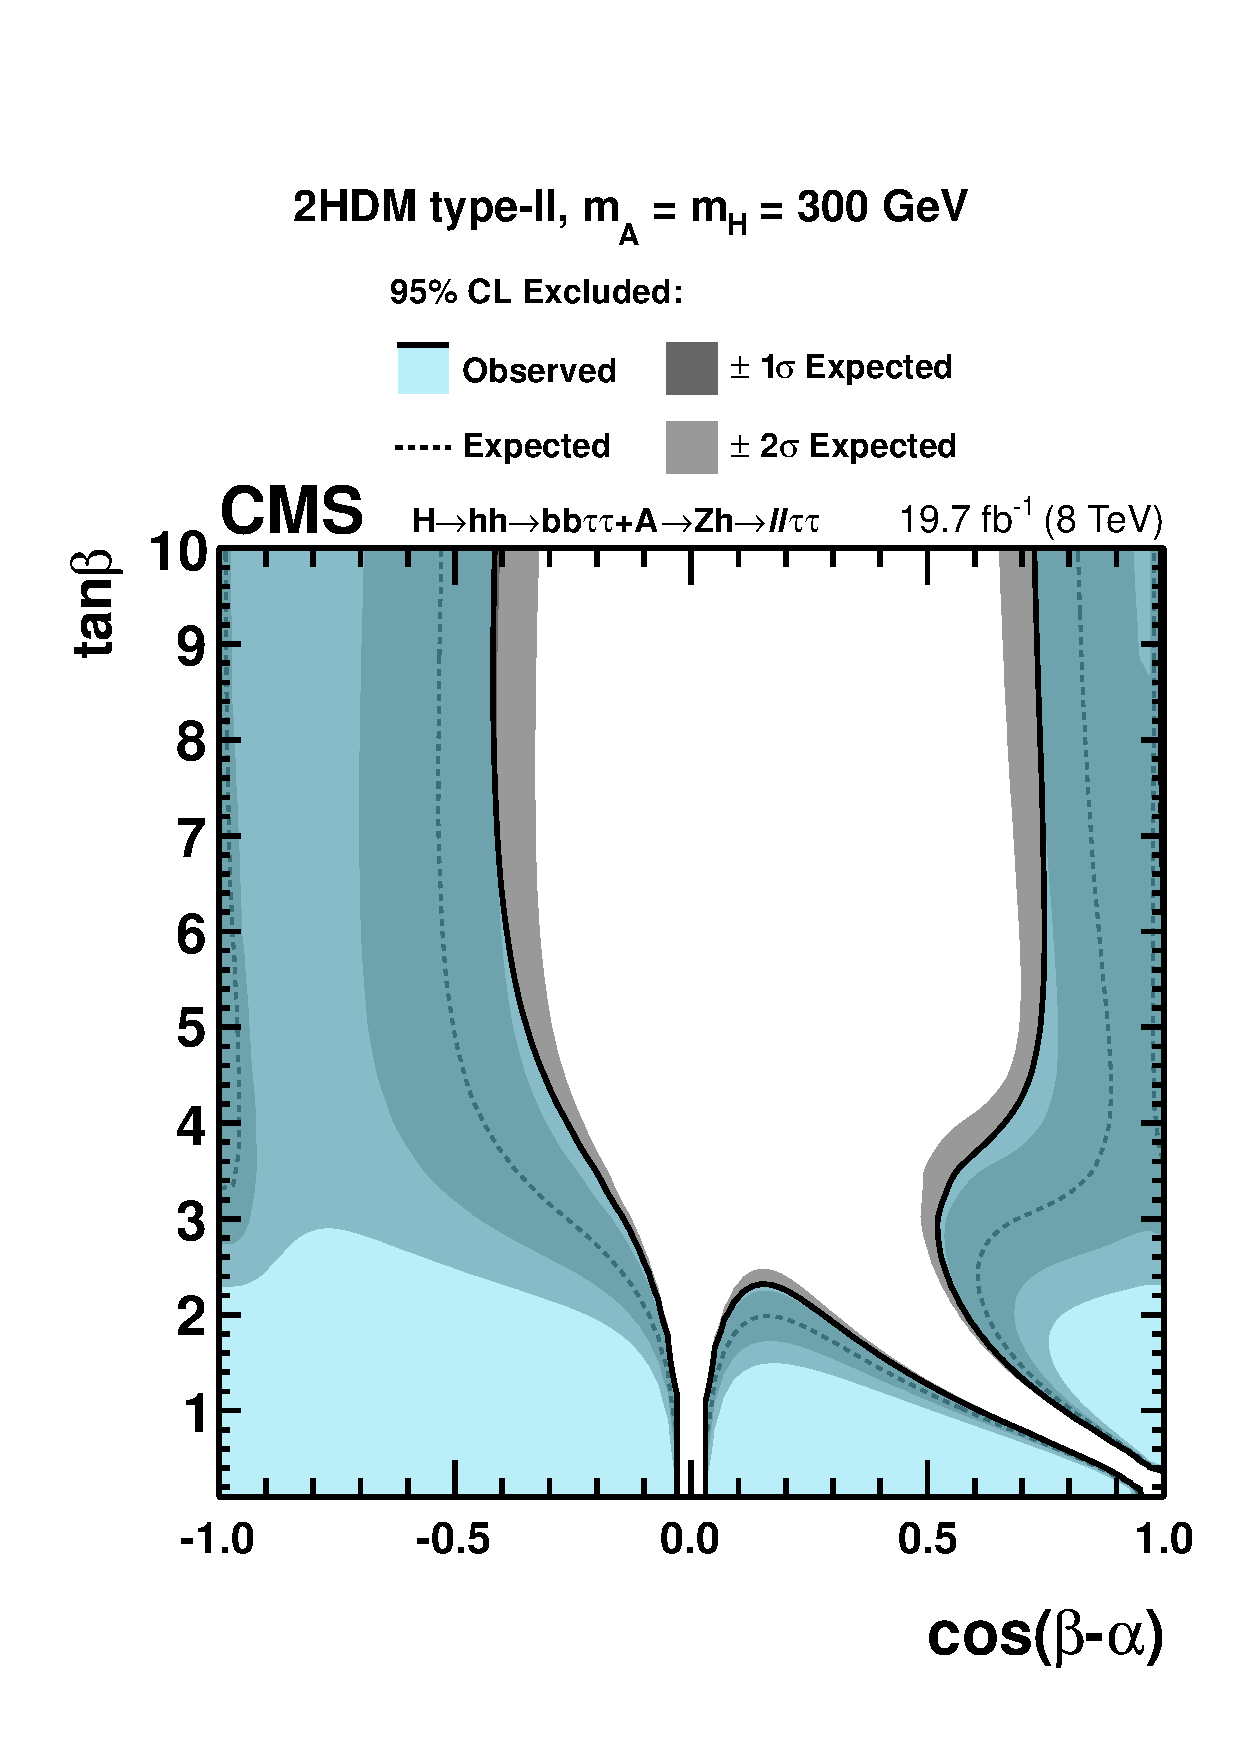
\includegraphics[width=0.85\textwidth]{Hhh/Plots/CMS-HIG-14-034_Figure_012.pdf}
%\caption{Combined interpretation of searches for \AtoZhtolltautau and 
%\Htohhtobbtautau in a type II 2HDM, assuming $m_{H} = m_{A} = m_{H^{+}} = 300$ GeV.
%The shaded blue area bounded by the solid black line indicates the observed 
%95\% confidence level excluded region. The dashed black line indicates the expected
%exclusion, with the grey bands indicating the $\pm 1\sigma$ and $2\sigma$ 
%exclusion limits \cite{CMS-HIG-14-034}.}
%\label{fig:HhhAZh2HDM}
%\end{center}
%\end{figure}


\begin{figure}[h!]
\begin{center}
\subfloat[type-II 2HDM]{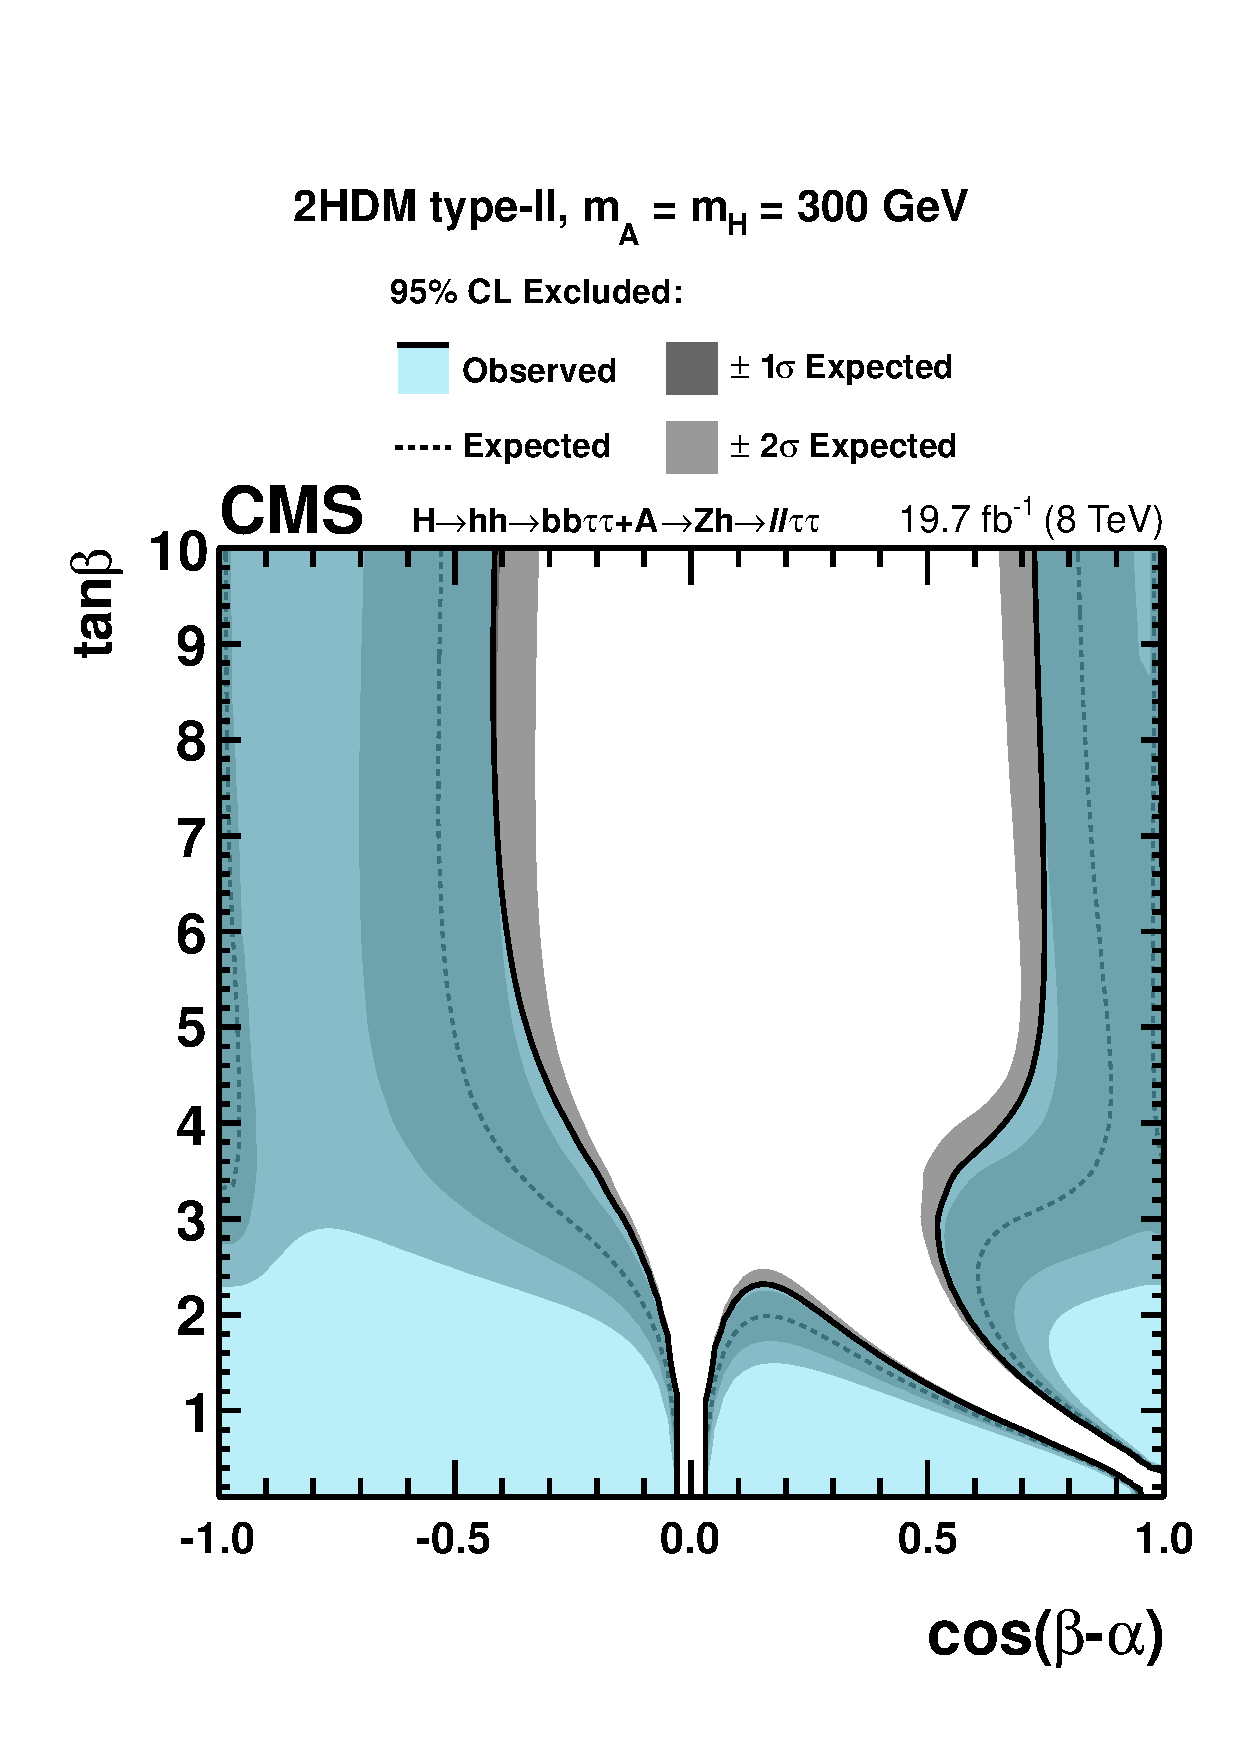
\includegraphics[width=0.5\textwidth]{Hhh/Plots/CMS-HIG-14-034_Figure_012.pdf}}
\subfloat[low-\tanb~MSSM scenario]{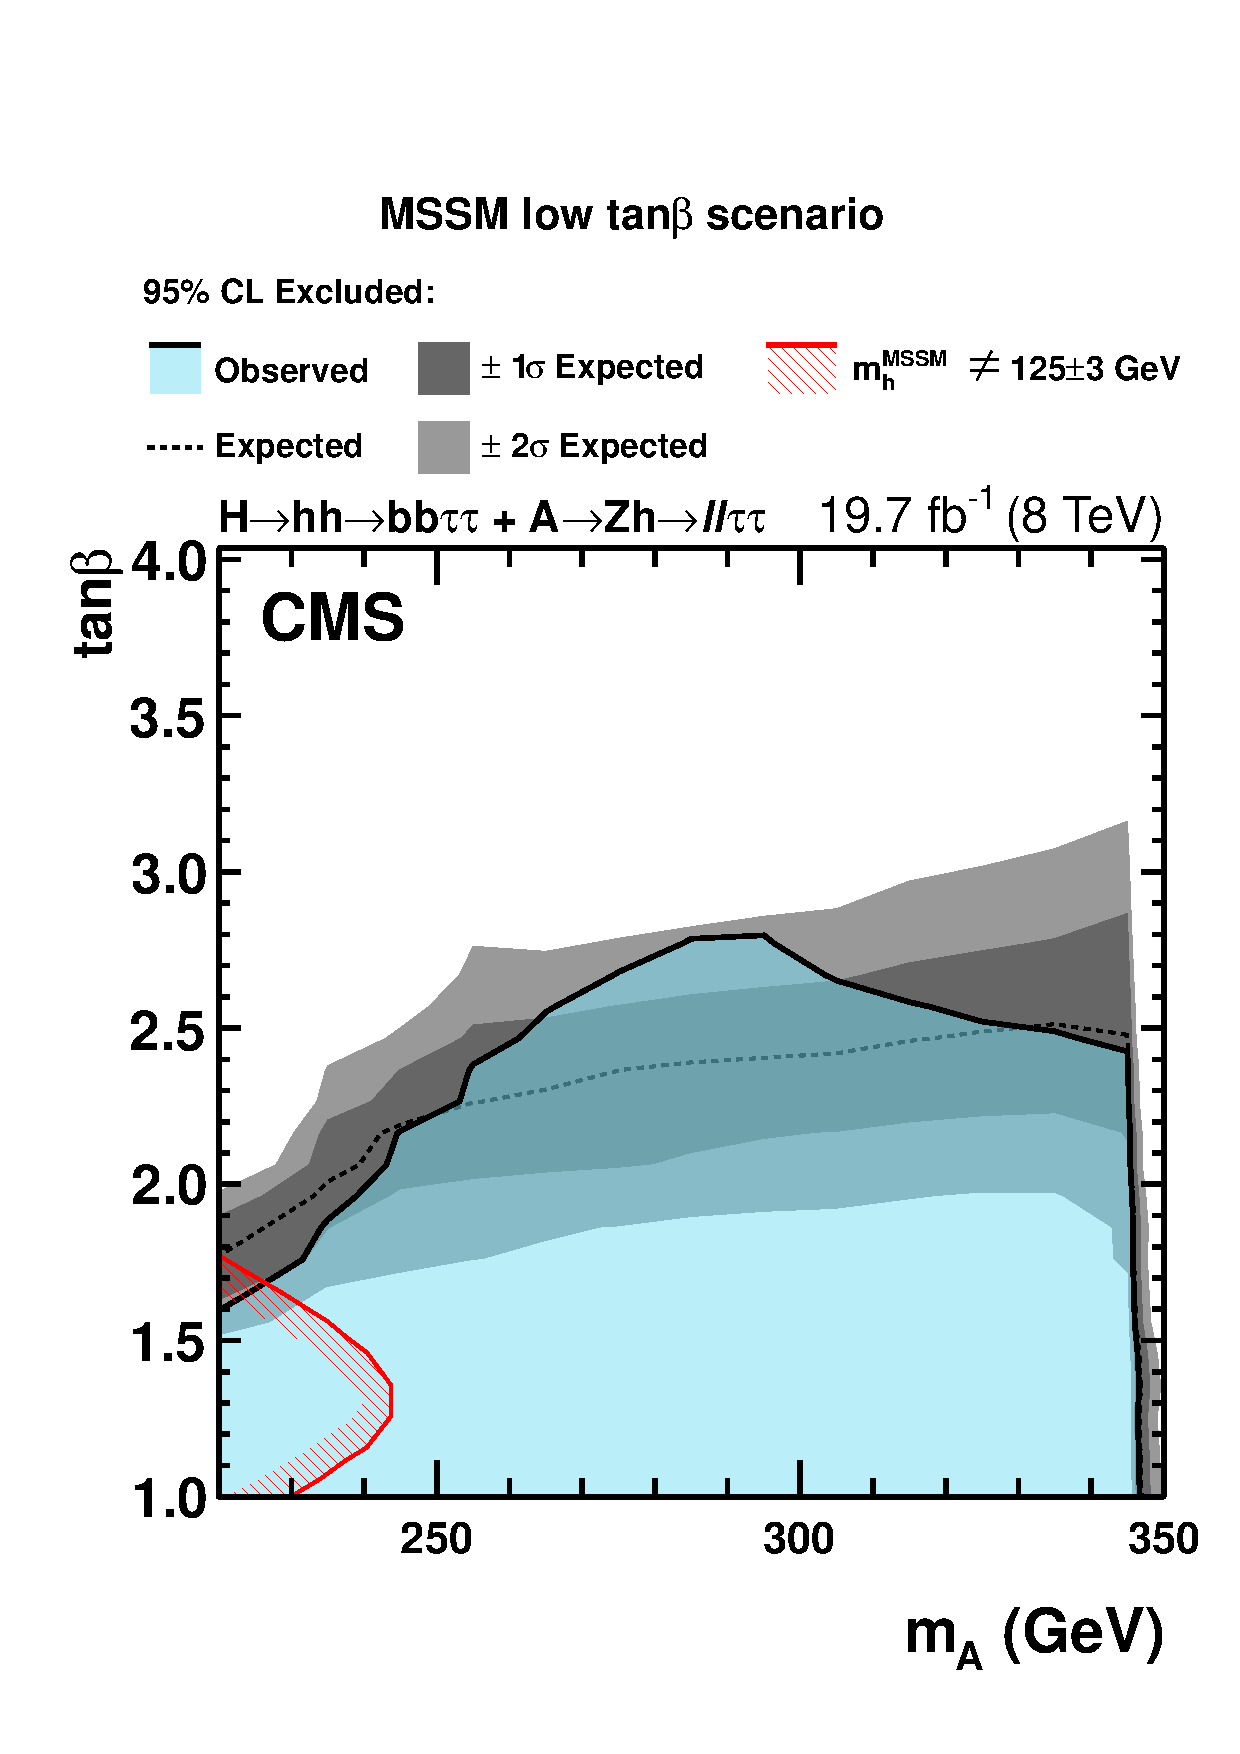
\includegraphics[width=0.5\textwidth]{Hhh/Plots/CMS-HIG-14-034_Figure_011.pdf}}
\caption[Combination of the \AtoZhtolltautau and \Htohhtobbtautau searches
interpreted in a type-II 2HDM and in the low-\tanb~MSSM scenario.]{Combination of the \AtoZhtolltautau and \Htohhtobbtautau searches
interpreted in (a) a type-II \ac{2HDM} assuming $m_{\PHiggs} = m_{\PHiggsps} = m_{\PHiggs^{+}} = 300\,\GeV$ and 
(b) in the low-\tanb~MSSM scenario. The shaded blue area bounded by
the solid black line indicates the observed excluded region at 95\% \ac{CL}.
The dashed black line indicates the expected exclusion, with the grey bands showing
the $\pm 1\sigma$ and $\pm2\sigma$ expected exclusion \cite{CMS-HIG-14-034}. The area
bounded by the red line is the region of phase space where \mh~$\neq 125 \pm 3\,\GeV$
 and is therefore excluded.}
\label{fig:HhhAZhMSSM2HDM}
\end{center}
\end{figure}
